\part[Nouvelles constructions linéaires et non-linéaires pour chiffres par bloc]
	{New linear and non-linear mappings for block ciphers}
\label{part:constructions}

\section*{Overview}

A widespread design type for block ciphers is the \emph{SPN} structure. Initially, this stood for \emph{substitution-permutation network},
with ``permutation'' referring to ``bit'' permutations; in its current usage, this term generally denotes arbitrary (\ftwo-)linear
mappings.

The rationale behind the SPN structure is that one may obtain a good block cipher round function by alternating a substitution
mapping made of the parallel application of \emph{S-boxes} (short for ``substitution boxes'') and a linear mapping. The role
of both mappings are complementary, and each is also usually selected to interact well with the other. While the S-boxes
are expected to break any exploitable structure (linear and algebraic, in particular) at the local level, the permutation
should spread the effects of the S-boxes at the global level, in particular to ensure that no local change remains so through
the entire cipher execution.

An advantage of SPNs over some other design structures is that they lend themselves relatively well to analysis, in particular w.r.t.
statistical attacks; this is exemplified by the \emph{wide-trail strategy} used in the design of the \aes. Another notable point
about SPNs is that they offer many possible tradeoffs in their instantiations. One can choose between large and small S-boxes,
large S-boxes are comparatively stronger than small ones, but also more expensive; best-performing S-boxes or cheaper
``average'' ones; bit permutations, particularly efficient in hardware, or (non-permutation) matrices; ``optimally diffusing'' (MDS)
matrices or not; state-wide matrices or not, etc.; the design space of SPNs is thus quite large.

\bigskip

In the second part of this thesis, we study two mappings intended to be used as part of an SPN round function, the second
of them being also instantiated in a complete block cipher design.

In \autoref{cha:difmat}, we present large linear mappings with very good diffusion and efficient software implementations,
with respect to their sizes. They are derived from linear codes over a small field (typically $\Fst$) with a high dimension
(typically 16) and a high minimum distance. This results in
diffusion matrices with equally high dimension and a large branch number.
Because we aim for parameters for which no MDS code is known to exist, we propose to use more flexible \emph{algebraic-geometry} codes.
We present two simple yet efficient algorithms for the software implementation of matrix-vector multiplication in this context, and derive
conditions on the generator matrices of the codes to yield efficient encoders. We then specify an appropriate code and use its automorphisms as well as random sampling
to find good such matrices.

In \autoref{cha:littlun}, we present
the construction and implementation of an 8-bit S-box with a differential and linear branch number of 3.
We show an application by designing \littlunpride: a simple block cipher
based on bitsliced evaluations of the S-box and bit rotations, which is designed to be efficient on 8-bit microcontrollers in particular.
The round function of \fly achieves good performance on its target platform, in terms of number of instructions per round and overall
code size, while providing good cryptographic properties.
The S-box also has an efficient implementation with SIMD instructions, a low implementation cost in hardware
and it can be masked efficiently thanks to its sparing use of non-linear gates and to the fact that it has a natural expression in
terms of a single 4-bit S-box.

\cleardoublepage
\chapter*{Contents}
\parttoc

%%%%%%%%%%%%%%%%%%%%%%%%%%%%%%%%%%%%%%%%%%%%%%%%%%%%%%%%%%%%%%%%%%%%%%%%
%%%%%%%%%%%%%%%%%%%%%%%%%%%%%%%%%%%%%%%%%%%%%%%%%%%%%%%%%%%%%%%%%%%%%%%%


%\chapter[Matrices de diffusions issues de codes géométriques]{Diffusion matrices from algebraic-geometry codes with efficent vector implementations}
\chapter[Matrices de diffusions issues de codes géométriques]{Efficient diffusion matrices from algebraic-geometry codes}
\label{cha:difmat}

\section{Introduction}

The use of \emph{MDS} matrices over finite fields as linear mappings in block cipher design is an old trend, followed by many prominent algorithms such as the \AES/\rijndael{} family~\cite{aes} and its predecessors~\cite{shark,square}.
These matrices are called MDS as they are derived from \emph{maximum distance separable} linear error-correcting codes, which achieve the highest minimum distance possible
for a given length and dimension. This notion of minimum distance coincides with the one of \emph{branch number} of a mapping~\cite{phddaemen}, which is a measure of the effectiveness
of a diffusion layer.
MDS matrices thus have an optimal diffusion, in a cryptographic sense, which makes them attractive for cipher design.

The good security properties that can be derived from MDS matrices are often counter-balanced by the cost of their computation. The standard matrix-vector product is
quadratic in the dimension of the vector, and finite field operations are not always efficient.
For that reason, there is often a focus on finding matrices allowing efficient implementations. For instance, the \AES{} matrix is circulant and has small coefficients.
More recently, the \photon{} hash function~\cite{photon} introduced the use of matrices that can be obtained as the power of a companion matrix, whose sparsity may be useful in
lightweight hardware implementations. The topic of finding such so-called recursive diffusion layers has been quite active in the past years, and led to a series
of papers investigating some of their various aspects~\cite{recursive1,recursive2,recursive3}. One recent development shows how to systematically construct some of these matrices
from BCH codes~\cite{recursive4}. This allows in particular to construct very large recursive MDS matrices, for instance of dimension sixteen over $\Fth$. This defines a linear mapping over
a full 128-bit block with excellent diffusion properties, at a moderate hardware implementation cost.

As interesting as it may be in hardware, the cost in software of a large linear mapping tends to make these designs rather less attractive than more balanced solutions.
An early attempt to use a large matrix was the block cipher \shark{}, a \rijndael{} predecessor~\cite{shark}; the same kind of design
was also later used for \khazad~\cite{khazad}. Both are  64-bit ciphers which use an MDS matrix of dimension
eight over $\Fth$ for their linear diffusion. The usual technique for implementing such a mapping in software is to rely on a table of precomputed multiples of
the matrix rows. However, table-based implementations now tend to be frown upon as they may lead to \emph{timing attacks}~\cite{timinattacks}, and this could
leave ciphers with a structure similar to \shark{}'s without reasonable software implementations when resistance to these attacks is required.
Yet, such designs also have advantages of their own; their diffusion acts on the whole state at every round, and therefore makes structural attacks harder,
while also ensuring that many S-Boxes are kept active.
Additionally, the simplicity of the structure makes it arguably easier to analyse than in the case of most ciphers.

\paragraph{Our contributions.}

In this chapter, we revisit the use of a \emph{\shark{} structure} for block cipher design and endeavour to find good matrices and appropriate algorithms
to achieve both a linear mapping with very good diffusion and efficient software implementations that are not prone to timing attacks.
To be more specific on this latter point, we target software running on 32 or 64-bit CPUs featuring an SIMD vector unit.

A possible way of making a mapping more efficient is to decrease the size of the field from $\Fth$ to $\Fst$. However, according to the \emph{MDS conjecture},
there is no MDS code over $\Fst$ of length greater than seventeen~\cite{mdsConj}. Because a diffusion matrix of dimension $n$ is typically
obtained from a code of length $2n$, MDS matrices over $\Fst$ are therefore restricted to dimensions less than eight. Hence, the prospect
of finding an MDS matrix over $\Fst$ diffusing on more than $8\times4 = 32$ bits is hopeless.
Obviously,
32 bits is not enough for a large mapping \emph{à la} \shark{}. We must therefore search for codes with a slightly smaller minimum distance
in the hope that they can be made longer.

Our proposed solution to this problem is to use \emph{algebraic geometry codes}, as they precisely offer this tradeoff.
One way of defining these codes is as evaluation codes on algebraic curves; thus our proposal brings a nice connection between these objects and
symmetric cryptography: although elliptic and hyperelliptic curves are now commonplace in public-key cryptography, we show an unusual application of
a hyperelliptic curve to the design of block ciphers. We present a specific code of length 32 and dimension 16 over $\Fst$ with minimum distance 15, which is only
two less than what an MDS code would achieve; this is also much better than a random code for these alphabet, length and dimension, as such a code
would typically have an expected minimum distance of 11.
This lets us deriving a very good diffusion matrix on $16\times4 = 64$ bits in a straightforward way. Interestingly, this matrix can also be applied
to vectors over an extension of $\Fst$ such as $\Fth$, while keeping the same good diffusion properties.
This allows for instance to increase the diffusion to $16\times8 = 128$ bits.

We also study two simple yet efficient algorithms for implementing the matrix-vector multiplication needed in a \shark{}
structure, when a \emph{vector permute} instruction is available. From one of these, we derive conditions on the matrix to make the matrix-vector product
faster to compute, in the form of a cost function; we then search for matrices with a low cost, both randomly, and by using automorphisms of the code and of the hyperelliptic
curve on which it is based. The use of codes automorphisms to derive efficient encoders is not new~\cite{sysgrob,grobarch},
but it is not generally applied to the architecture and dimensions that we consider in our case.

We conclude the chapter by presenting examples of performance figures of assembly implementations of our algorithms when used as the linear mapping of
a block cipher.


\section{Preliminaries}
\label{not}

We introduce a few notations, definitions and background notions that are used in this chapter. We illustrate some of these with classical examples, such as \emph{Reed-Solomon} codes. However,
our goal is not to provide a detailed exposition on coding theory, and we refer the reader to any good textbook such as \cite{vanlint} for a thorough treatment.

\subsection{Notations}
We write `$\defas$' equality by definition.
We note $\Fq$ an arbitrary finite field and \Ftwom{} the finite field with $2^m$ elements. We often consider $\Fst$, and implicitly use this specific field if not mentioned otherwise.
W.l.o.g. we use the representation
$\Fst \cong \mathbf{F}_2[\alpha]/(\alpha^4 + \alpha + 1)$ when a specific one is needed. We freely use ``integer representation'' for elements of $\Ftwom \cong \Ftwom[\alpha]/I(\alpha)$
by writing $n \in \{0\ldots2^n-1\} = \sum_{i = 0}^{n-1} a_i 2^i$ to represent the element
$x \in \Ftwom = \sum_{i = 0}^{n-1} a_i \alpha^i$. In the remainder of this section, and especially in \autoref{sec:ag}, we usually consider an arbitrary algebraically closed field, written $k$
(it will usually be clear from the context whether $k$ is a field or the dimension of a linear code, see \autoref{def:lincode} below).
$\mathfrak{S}_n$ denotes the group of permutations of $n$ elements.

Bold variables denote vectors (in the sense of elements of a vector space), and subscripts are used to denote their $i^\text{th}$ coordinate, starting from zero. For instance,
let $\veci \defas (1, 2, 7)$, then  $\veci_2 = 7$.
If $\mat$ is a matrix of $n$ columns, we call $\mat_i \defas (\mat_{i,j},~j = 0\ldots n - 1)$ the row vector formed from the coefficients of
its $i^\text{th}$ row.
We use angle brackets ``$\langle$'' and ``$\rangle$'' to delimit ordered sets.

Arrays, or tables, (in the sense of software data structures) are denoted by regular variables such as $x$ or $T$, and their elements are accessed by using square brackets.
For instance, $T[i]$ is the $i^\text{th}$ element of the table $T$, starting from zero.

The operator ``$\wedge_{64}$'' denotes the  \emph{logical and} on 64-bit values. We use $\mathbf{0}_{n}$ and $\mathbf{1}_n$ for binary vectors of length $n$ all made of
zeros and ones respectively. If $n$ is a multiple of a power of two, these vectors may freely be interpreted as elements of the relevant vector spaces.
The function $\indic(\cdot)$ takes as input a set and returns one if it is non-empty, zero otherwise; $\#$ denotes the cardinality of a set.
We may also use subscripts to show the base in which a number is written when it is not ten, \eg $1010_2$ is the number 10 written in base two.

% We may use the term ``vector'' as well to denote such variables,
% but the notation should make it clear if we mean a logical array or an element of a vector space; sometimes both notions might coincide.

%Other notations or specific variables are introduced when they are needed, and keep their meaning through the remainder of the text if not otherwise stated.
%Some background notions might not be redefined if they are not deemed to be essential for the understanding of the paper.

\subsection{Linear codes}

\begin{defi}[Hamming weight, Hamming distance]
Let $\veci$ be a vector of $k^n$. Its \emph{Hamming weight} $\weight(\veci) \in [0,\ldots,n]$ is $\#\{\veci_i, i = 0,\ldots,n-1~|~ \veci_i \neq 0\}$,
the number of its coordinates which are non-zero.
The \emph{Hamming distance} $\hdist(\veci,\veco)$ between two vectors is defined as $\weight(\veci - \veco)$.
\end{defi}


\begin{defi}[Linear code]
\label{def:lincode}
A \emph{linear code} of \emph{length} $n$, \emph{dimension} $k$ and \emph{minimal distance} $d$ over the alphabet $\Fq$ is a $k$-dimensional linear subspace of $\Fq^n$ such that $\veci, \veco \in \code \Rightarrow \hdist(\veci, \veco) \geq d$
and $\exists \veci, \veco \in \code,  \hdist(\veci, \veco) = d$.
The last conditions can equivalently be expressed as $\veci \neq \nullvec \in \code \Rightarrow \weight(\veci) \geq d$ and $\exists \veci \in \code, \weight(\veci) = d$.
We use the usual ``NKD'' notation to characterize codes: an $[n, k, d]_{\Fq}$ code $\code$ is a code of length $n$, dimension $k$ and minimum distance $d$
with symbols in \Fq.
\end{defi}

We only consider linear codes in this manuscript and we will therefore omit this qualifier in the remainder of the text. 
We usually view a code as a set, and call \emph{codewords} its elements. By an abuse of terminology, we may call \emph{messages} the elements of $\Fq^k$.

\begin{defi}[Dual code]
Let $\code$ be an $[n, k, d]_{\Fq}$ code over $\Fq$ equipped with a scalar product $\langle\cdot,\cdot\rangle$. The \emph{dual}
$\code^\bot$ of $\code$ is defined as $\{\veci \in \Fq | \forall \veco \in \code, \langle\veci,\veco\rangle = \nullvec\}$.
\end{defi}

A code $\code$ equal to its dual $\code^\bot$ is called \emph{self-dual}.


\begin{defi}[Generator matrix, systematic form]
A \emph{generator matrix} $G$ of an $[n, k, d]_{\Fq}$ code $\code$ is a matrix of $\matspace_{k,n}(\Fq)$ such that
$\code = \{\veci G, \veci \in \Fq^k\}$. It is in \emph{systematic form} if it is of the form $(I_k~A)$ with
$I_k$ the identity matrix of dimension $k$. 
\end{defi}

If $(I_k~A)$ is a generator matrix for a code $\code$, then $(-A^t~I_{n-k})$ (or equivalently $(I_{n-k}~-A^t)$)
is a generator matrix for its dual $\code^\bot$. It follows that if $\code$ is self-dual, $A$ is symmetric and
orthogonal.
% TODO why not just A.A^t diagonal?

\begin{defi}[MDS code, MDS matrix]
An $[n,k,d]_{\Fq}$ code $\code$ is called \emph{maximum distance separable}, or simply \emph{MDS}, if $d = n - k + 1$.
By abuse of definition, if $n = 2k$ and $(I_k~A)$ is a generator matrix of $\code$, we call $A$ an \emph{MDS matrix}.
\end{defi}

It is easy to see that this is the highest possible minimum distance that can be achieved by a code with a
systematic generator matrix, as all rows of such a matrix have weight at most $n - k + 1$.

A useful alternative characterization of MDS matrices is given by the following theorem.

\begin{thm}[\cite{mdsConj}]
\label{thm:mds_minors}
A matrix $M$ is MDS if and only if all of its minors are non-zero (\ie all the square sub-matrices of $M$ are invertible).
\end{thm}

A consequence of this is that the dual of an MDS code is also MDS.
We also have the following (in simplified form):

\begin{conj}[MDS conjecture]
There is no MDS code with symbols in $\Fu$ of length $n$ with $n > \#\Fu + 1$\footnote{This maximal length can be increased by one
for some values of $q$ and $k$.}.
\end{conj}

The next definition rephrases and generalizes some of the above concepts in a way that is more suitable to cryptographic applications.
We assume in this case that $\Fq = \Ftwom$ for some $m$.

\begin{defi}[Branch number~\cite{aes}]
Let $A$ be the matrix of a linear mapping over $\Fu$.
The \emph{differential branch number} of $A$
is equal to $\min_{\veci \neq 0}(\weight(\veci) + \weight(\veci A))$,
and the \emph{linear branch number} of $A$ is equal to $\min_{\veci \neq 0}(\weight(\veci) + \weight(\veci A^t))$.
\end{defi}

If $A$ is such that $(I_k~A)$ is a generator matrix of a code of minimum distance $d$ which dual has minimum distance $d'$,
then $A$ has a differential (resp. linear) branch number of $d$ (resp. $d'$).

\subsubsection{Evaluation codes}

The algebraic-geometry codes that we use in this chapter are conveniently defined as instantiations of the general framework of \emph{evaluation codes}, for which
we give a brief overview.
We start with a general definition:

\begin{defi}[Evaluation code]
Let $\funcspace$ be an $\Fq$-vector space of dimension $k$ of functions $\fun : \dom \rightarrow \Fq$ (the \emph{function space}). Let $\points \defas \langle P_0,\ldots, P_{n-1}\rangle$
be an ordered subset of $\dom$ of cardinality $n$ (the \emph{evaluation domain}). Let $\evmap_\points : \funcspace \rightarrow \Fq^n$ be the \emph{evaluation map}
defined as $\evmap_\points(\fun) \defas (\fun(P_0),\ldots,\fun(P_{n-1}))$.
The \emph{evaluation code} $\evcode(\funcspace,\points)$ for an injective evaluation map $\evmap_\points$ is defined as $\{\evmap_\points(\fun)~|~\fun \in \funcspace\}$.
It is an $[n,k,\ast]_{\Fq}$ code.
\end{defi}

A generator matrix $G$ of an evaluation code can easily be constructed by evaluating a basis for $\funcspace$ on $\points$. Call $(\fun_0,\ldots,\fun_{k-1})$
such a basis, then $G = (\evmap_\points(\fun_0),\ldots,\evmap_\points(\fun_{k-1}))$.
If the code admits a systematic generator matrix, it can simply be obtained by computing the reduced row echelon form of $G$.

We use ordered sets for the evaluation domain $\points$ in this definition. Although the order that is chosen does not impact the parameters of the code (hence we
may sometimes abuse our definition and talk about \emph{the} code for any of the codes based on the same $\funcspace$ and $\dom$), it may have
an influence on the performance of explicit instantiations, through \eg properties of the generator matrices. Most of the work
of this chapter is actually based on this fact.

The probably best-known evaluation codes are the \emph{Reed-Solomon codes} (``RS codes''):

\begin{defi}[Reed-Solomon codes]
An $[n,k,\ast]_{\Fq}$ \emph{Reed-Solomon} code is an evaluation code obtained by taking $\funcspace$ to be the polynomials $\Fq[x]$
of degree less than $k-1$ and $\points$ any ordered subset of $\Fq$. 
\end{defi}

As we must have $n \geq k$ by definition of a code, all polynomials of $\funcspace$
can be uniquely interpolated on any $n$ points, hence $\evmap_\points$ is injective and Reed-Solomon codes are well-defined.
Furthermore, for any $\points$, any non-zero polynomial of $\funcspace$ is zero on at most $k - 1$ positions. The minimal distance of a Reed-Solomon code is thus $n - (k - 1)$, which makes them MDS codes.


\section{Algebraic-geometry codes}
\label{sec:ag}

We now present \emph{algebraic-geometry codes} (``AG codes''), which are the main object used in this chapter,
and we show how they can give rise to diffusion matrices with interesting parameters.
We introduce a few geometry notions along the way in order to be able to faithfully describe the codes we will
be using. 
We refer the reader to the relevant chapters of \cite{vanlint,tvn,stichtenoth,fulton} for a much more detailed and rigorous treatment of the subject. 

\paragraph{AG codes as a generalization of RS codes.}
We first give an intuition of the construction used in AG codes. We have seen that RS codes are MDS
and that they can be instantiated for many lengths and dimensions. One limitation of the construction
is that the maximal length of the code is limited by the cardinality of the alphabet $\Fq$: we
cannot evaluate the functions on more points than there are elements in $\Fq$ without introducing some
repetition; we can still slightly increase this maximal length by one (two for some
very very specific and uncommon values of $k$ and $q$) by defining an \emph{extended} RS code, which is still MDS. However, by the MDS
conjecture, we do not expect to be able to do better than that.
Yet we may want to
have a tradeoff between the maximal length of a code construction and its \emph{designed minimal distance} $d^* \leq d$.

A natural way to increase the maximal length of an evaluation code is to consider functions over domains
of higher dimension than the ``line'' used in RS codes. For instance, one could take $\dom$ to be the
$m$-dimensional space $\Fq^m$, and $\funcspace$ to be the $m$-variate polynomials of $\Fq[x_0,\ldots,x_{n-1}]$
less than a certain degree $r$. This defines \emph{Reed-Muller codes} (``RM codes'') of order $r$.
Although this construction successfully yields codes longer than RS codes, they are not asymptotically good\footnote{An
$[n, k, d]$ code si asymptotically good if neither of $d/n$ and $k/n$ tends to zero when $n$ goes to the infinity.}.

An alternative approach to construct longer variants of RS codes is the one followed by AG codes. Seeing
RS codes as working with a line of genus zero, the idea is to take as evaluation domains
the points of curves of higher genera (planar and affine in our case, so as not to complexify things too much),
which can be assimilated to a subset of $\Fq^2$. A geometrically
meaningful way to choose the function space $\funcspace$ is then to consider certain subspaces of
the function fields of the curves. We will see that for well-chosen $\funcspace$, this construction
leads to codes of parameters $[n, k, d \geq n - k + 1 - g]_{\Fq}$ for curves of genus $g$. As the
(maximal) number of points on a curve is roughly increasing with the genus, this construction gives us the
sort of tradeoff we were searching for.

\subsection{Selected algebraic geometry notions}

We will be needing a few tools from algebraic geometry to make our description of AG codes explicit. We only introduce
here the notions that are relevant to this specific application,
largely ignoring the wider picture. Note that unlike the remainder of this chapter, the underlying fields used in the definitions
are not necessarily finite.

As we see AG codes as evaluation codes, we need to be able to: 1) Describe the evaluation domains.
2) Define the function spaces $\funcspace$ associated with given evaluation domains,
and be able to compute their bases.

\medskip

The construction of the examples of AG codes that we later consider can eventually be described in a purely affine way. However, in order to
justify them, we need to be able to reason about points at infinity. Thus we start with the following:

\begin{defi}[Affine space, projective space]
\label{def:affiprojec}
The $n$-dimensional \emph{affine space} $\affi^n(k)$ over a field $k$ is a set of \emph{points} formed by $n$-tuples over $k$,
$P \defas (x_0, \ldots, x_{n-1})$, $x_i \in k$.
The $n$-dimensional \emph{projective space} $\projec^n(k)$ over $k$ is a set of points formed by equivalence classes of $(n+1)$-tuples
$P \defas (x_0 : \ldots : x_n)$, $x_i \in k$, where not all $x_i$s are zero, and the equivalence relation $\sim$ is
defined by $(x_0 : \ldots : x_n) \sim (\lambda x_0 : \ldots : \lambda x_n)$, $\lambda \in k^*$. In the (usual) case where $n = 2$, we let
$x \defas x_0$, $y \defas x_1$ and $z \defas x_2$.

\noindent
The space $\affi^n(k)$ can be embedded into $\projec^n(k)$ in a natural way as $(x_0, \ldots, x_{n-1}) \mapsto (x_0 : \ldots : x_{n-1} : 1)$.
The set of projective points $(x_0 : \ldots : x_{n-1} : 0)$ is called the \emph{hyperplane at infinity}.
\end{defi}

We now define projective varieties.

\begin{defi}[Projective variety]
A \emph{projective variety} in the projective space $\projec^n(k)$ over an algebraically closed field $k$ is the set of common zeros
of a prime ideal $\mathcal{I} \defas \langle f_0, \ldots, f_m \rangle$ of homogeneous polynomials of $k[x_0,\ldots,x_n]$ (a polynomial is called \emph{homogeneous}
if all its monomials have the same degree).
\end{defi}

A \emph{projective curve} is a projective variety of dimension one\footnote{The dimension $n$ of a variety $V$ is defined by
the maximal length of the inclusion chain $V = V_0 \supset \ldots \supset V_n \neq \emptyset$, with $V_i$ closed in $V_{i-1}$ (for the \emph{Zariski topology})
for all $i \in \{1,\ldots,n\}$.}. In practice, we will only consider curves in $\projec^2$ (plane curves),
which will then be defined by a single homogeneous polynomial $E$.

\paragraph{Remarks.}
\begin{enumerate}
\item The condition that $k$ be algebraically closed is not as restrictive as it may seem. Say that we wish to work in $\Fq$ (meaning in particular
that all coefficients of $E$ are in $\Fq$); though we will define a curve $\curve$ over the algebraic closure of $\Fq$, we
will only be interested in $\curve(\Fq)$, the points of $\curve$ that lie in $\Fq$ (its \emph{$\Fq$-rational points}, or simply rational points). 
\item For a given projective variety, say $\curve$ defined by $E(x,y,z)$, one can consider the corresponding affine variety defined as the zeros of ``$E(x,y,1)$,
$E \in k[x,y]$'' (the ``dehomogenised'' of $E$). It will have the same points (in the sense of the embedding of \autoref{def:affiprojec}) as $\curve$, minus its potential points at infinity.
Similarly, an affine variety can be extended to its projective closure.
\end{enumerate}

Our first step towards defining suitable function spaces $\funcspace$ is to define the function field of a variety.
We give two definitions, one in the affine and one in the projective case.

\begin{defi}[Coordinate ring, function field of an affine variety]
Let $\curve$ be an affine variety in $\affi^n(k)$ defined by the ideal $\mathcal{I}$. The \emph{coordinate ring} $k[\curve]$ of $\curve$ is $k[x_0, \ldots, x_{n-1}]/\mathcal{I}$.
The \emph{function field} $k(\curve)$ of $\curve$ is the quotient field of $k[\curve]$.
\end{defi}

\begin{defi}[Function field of a projective variety]
Let $\curve$ be an affine variety in $\projec^n(k)$ defined by the ideal $\mathcal{I}$. Let $F$, $G$ be homogeneous polynomials of equal degrees in $k[x_0, \ldots, x_n]$
with $G \notin \mathcal{I}$. The \emph{function field} $k(\curve)$ of $\curve$ is the set of \emph{rational functions} $F/G$ modulo $\mathcal{I'}$,
where $\mathcal{I'} = \{F/G~|~ F \in \mathcal{I}\}$.

\noindent
A rational function $F/G$ is \emph{regular} at $P$, point of $\curve$, if $G(P) \neq 0$.
\end{defi}

We will need to be able to talk about the behaviour of functions at specific points of a curve. For this, we first use the following:

\begin{defi}[Local ring of a point]
The \emph{local ring} $\locring_P$ of a point $P$ of a variety $\curve$ is the set of rational functions regular at $P$.
It has a unique maximal ideal $\maxi_P \defas \{f \in \locring_P ~|~ f(P) = 0\}$. 
\end{defi}

The local ring and its maximal ideal are in particular useful to define the \emph{tangent space} at a point $P$, which in turn allows to define smooth and singular points,
depending on its dimension.
We will not give the general definition here, mentioning instead  the following convenient alternative characterization in the specific case of curves:

\begin{defi}[Smooth and singular points of a curve, local parameter]
A point $P$ of a curve $\curve$ is \emph{smooth} or \emph{non-singular} iff $\maxi_P$ is a principal ideal. Any generator of the ideal ($t_P \in \locring_P$ s.t. $\maxi_P = t_P\locring_P$)
is called a \emph{local parameter} at $P$.

\noindent
A point that is not smooth is called \emph{singular}.
\end{defi}

To build an AG code from a curve $\curve$, we will require that it is smooth, \ie that none of its points are singular.
% (actually, we will
%only require this for $\curve(\Fq)$ for some $\Fq$).
We only consider smooth curves until \autoref{sec:nonsingmod}.

The local parameters are useful in defining the order of zeros and poles of arbitrary rational functions at a given point.
Let $f \neq 0$ be a rational function regular at $P$ and $t_P$ be a local parameter at $P$. The \emph{order} of $f$ at $P$ is:
\[
\ord_P(f) \defas \max \{k~ |~ f \in t_P^k\locring_P,~ f \notin t_P^{k+1}\locring_P\}.
\]
This can be extended to arbitrary rational functions by writing them as quotients of functions of $\locring_P$:
\[
\ord_P(f/g) = \ord_P(f) - \ord_P(g),~f,g\in\locring_P.
\]
For a function $f$, if $\ord_P(f) \geq 0$, we call this value the \emph{zero order} of $f$ at $P$; if $\ord_P(f) < 0$
we call $-\ord_P(f)$ the \emph{pole order} of $f$ at $P$.

We note in particular the two useful properties of $\ord$:
1) $\ord(fg) = \ord(f) + \ord(g)$; 2) $\ord(1/f) = -\ord(f)$.

%We will shortly see that being able to compute the order of a function at some desired points is essential in the definition of $\funcspace$.
In effect, $\ord_P$ defines a \emph{discrete valuation} of functions of $k(\curve)$, associated with the point $P$, \ie $\locring_P$ is a \emph{valuation ring}:

\begin{defi}[Valuation ring]
A ring $\locring$ is a \emph{valuation ring} of $k(\curve)$ if $k \subset \locring \subset k(\curve)$  and for every $f \in k(\curve)$,
$f \in \locring$ or $f^{-1} \in \locring$.
\end{defi}

We will see shortly that the ability to define valuations at any point is essential
in the definition of our function space $\funcspace$; this is why we require the curve to be non-singular, as a local ring is a valuation ring iff $P$ is smooth.

\medskip

The last main objects that we introduce are the divisors on a curve.

\begin{defi}[Divisor]
A \emph{divisor} on a smooth curve $\curve$ is a formal (finite) sum of points $P_i$ of $\curve$: $D \defas \sum a_iP_i$, $a_i \in \mathbf{Z},~P_i \in \curve$.
The \emph{support} of a divisor is the set of points $P_i$ with $a_i \neq 0$.

\noindent
The set $\cdiv(\curve)$ of divisors on $\curve$ with formal addition and negation of divisors ($\sum a_iP_i + \sum b_iP_i \defas \sum (a_i+b_i)P_i$;
$-\sum a_iP_i \defas \sum -a_iP_i$) forms a group.

\noindent
A divisor $D \defas \sum a_iP_i$ is called \emph{effective} ($D \geq 0$) if $\forall i,~a_i \geq 0$.

\noindent
The \emph{degree} $\deg(D)$ of $D = \sum a_iP_i$ is defined as $\sum a_i$
\end{defi}

\begin{defi}[Divisor of a rational function (principal divisor)]
The divisor $(f)$ of a rational function $f \in k(\curve)$, $f \neq 0$, is defined as $\sum \ord_P(f)P$.
A divisor $D$ equal to $(f)$ for some function $f$ is called a \emph{principal divisor}.
\end{defi}

Principal divisors form a subgroup of $\cdiv(\curve)$. It can be shown that they are always of degree zero
(this is equivalent to saying that a rational function always has the same number of poles and zeros, counted with
multiplicity).

\begin{defi}[Space associated with a divisor]
Let $D \in \cdiv(\curve)$. We define $\rrs(D)$, the \emph{space associated with $D$} (or \emph{Riemann-Roch space}) as:
\[
\rrs(D) = \{f \in k(\curve)^*~|~(f) + D \geq 0\} \cup \{0\}.
\]
This forms a $k$-vector space; we write $\ell(D)$ its dimension.
\end{defi}

This is finally the kind of function space we will be using to define AG codes. For a divisor
$D \defas \sum a_iP_i - \sum b_jP_j$, $a_i, b_j \geq 0$, a simple reformulation of $\rrs(D)$ is to say that it consists of the zero function and of all the functions
which may have poles only in the $P_i$s of order at most $a_i$, and which must have zeros in all the $P_j$s of order
at least $b_j$.

It can be shown that for any $D$, $\rrs(D)$ is finite-dimensional. In fact, this is a consequence of two major theorems first from Riemann and then extended by Roch, which allow in particular to compute the explicit value $\ell(D)$
for a given divisor $D$~; this is expressed by the following corollary:

\begin{cor}[Corollary of Riemann and Roch]
Let $D$ be a divisor on a curve of \emph{genus} $g$, then $\ell(D) \geq \deg(D) + 1 - g$, with equality
when $\deg(D) > 2g - 2$.
\end{cor}

The formulation of this theorem uses the notion of \emph{genus} of a curve, that we have not defined yet. A possible, purely algebraic definition is precisely to take
$g(\curve) \defas \max \{\deg(D) - \ell(D) + 1,~D \in \cdiv(\curve)\}$. Although this is not very satisfying, we will not provide a better definition here (and computing
the genus in this way is not as hard as it may seem); in practice, the genus
of the curves we use will be known beforehand.

\subsubsection{Working with singular curves}
\label{sec:nonsingmod}

In the last few paragraphs, we have assumed that we were working with a smooth curve. We justified this by the need of being able to define a valuation for functions
at any point of the curve, which allowed us to define divisors and their associated vector spaces.
Unfortunately, some of the curves we may wish to use in practice are not smooth. We briefly and informally sketch here how it is possible to nonetheless work with some
of these curves. We refer the reader to \eg Fulton~\cite[Chap. 7]{fulton} for a serious treatment of the matter.

A first remark is that what effectively matters in the definition of the function space is not so much the points on the curves as their associated valuation
rings. It is in fact possible to define entirely what we have presented above in a purely algebraic way, as is done for instance by Stichtenoth~\cite{stichtenoth}.
In this case, the notion of points is replaced by the one of \emph{places} of a function field (written $F/k$, not necessarily associated with a curve), where a place is simply the (necessarily unique) maximal
ideal of a valuation ring of the function field:

\begin{defi}[Place of a function field]
A place $P$ of a function field $F/k$ is the maximal ideal of a valuation ring $\locring$ of $F/k$. 
\end{defi}

Divisors can then be redefined as sums of places instead of sums of points.

For a smooth curve $\curve$, there is a bijection between its points and the valuation rings (the places) of $k(\curve)$, and the theory as presented above is sufficient.
On the other hand, if $\curve$ is singular, we would like to be able to find a way of defining places at (some of) its singularities, on top of the smooth points.
This can be done by constructing a \emph{non-singular model} $\nscurve$ of $\curve$,
and taking as places of $\curve$ the points of $\nscurve$. A useful theorem is that for a projective curve $\curve$, there is a unique (up to isomorphism) non-singular curve
$\nscurve$ that is birationally equivalent to it\footnote{This means that there are \emph{rational maps} from $\curve$ to $\nscurve$ and vice-versa, that compose to the identity wherever they are
defined.
A rational map $\curve \subseteq \projec^m \rightarrow \projec^n$ is an $n+1$-tuple of homogeneous polynomials s.t. the polynomials do not jointly
vanish at any point of the curve.}. Furthermore, the function fields $k(\curve)$ and $k(\nscurve)$ are the same, up to isomorphism, so defining the places of $\curve$ in this
way is meaningful.
(We will not address here the problem of computing these non-singular models \emph{per se}.)

The map $\curve \rightarrow \nscurve$ may not be defined on every point of $\curve$, but the number of points where it is not defined is finite (this makes sense, as a curve
has at most finitely many singular points). We say that a place is \emph{centered} at a point $P$ if $P$ is its image by the map $\nscurve \rightarrow \curve$. Any non-singular
point of $\curve$ has exactly one place centered at it, while finitely many places may be centered at singular points.

We conclude by defining curves that are said to be in \emph{special position} (cf. \eg \cite{DBLP:journals/tit/SaintsH95}), which are convenient to use for several reasons.

\begin{defi}[Curve in special position]
A projective plane curve $\curve$\footnote{We recall our notations: a point $P \in \projec^2(k)$ is written $(x : y : z)$, and is
at infinity iff $z = 0$.} is in \emph{special position} if:
\begin{enumerate}
\item it has exactly one point $P_\infty$ at infinity;
\item there is exactly one place centered at $P_\infty$;
\item the affine curve $\curve_A \defas \curve\backslash P_\infty$ is smooth;
\item the pole order of $x/z$ and $y/z$ at $P_\infty$ are not equal.
\end{enumerate}
\end{defi}

Curves in special positions are useful as there is a bijection between their places and their points (even if they are potentially singular); thus they can always be considered
``as if smooth'' w.r.t. to the discussions of this section. Additionally, if one considers the space $\rrs(aP_\infty)$, $a > 0$, of functions having poles only at the point at infinity,
its elements can be mapped to polynomials of the coordinate ring of $\curve_A$. In other words, one can perform all the computations in $\rrs(aP_\infty)$ with the affine curve
only (we discuss how to explicitly compute bases for such spaces next). The main curve used in this chapter is a singular curve in special position.

\subsubsection{Computation of a basis of $\rrs(aP_\infty)$ for a curve in special position}

We conclude this brief presentation of algebraic curves and their function fields by showing how to compute a basis of $\rrs(aP_\infty$), $a > 0$
for a plane curve in special position.

Consider $\curve$ defined by a homogeneous equation $E(x,y,z)$. From a local parameterization at the place $P_\infty$, we can compute the pole order of
$f \defas x/z$ and $g \defas y/z$ at $P_\infty$ (which is enough to determine the pole
order of any fraction of $x$, $y$ and $z$).
An element of $\rrs(aP_\infty)$ is a linear combination $\sum_\alpha \alpha f^{\alpha_i}g^{\alpha_j}(z/z)^{\alpha_k}$ s.t. $\alpha_i + \alpha_j + \alpha_k$ is constant (the function is
homogeneous) and $\forall \alpha,~\alpha_i\ord_{P_\infty}(f) + \alpha_j\ord_{P_\infty}(g) \leq a$ (the pole order at $P_\infty$ of the monomials is less
than $a$).
A generating family for $\rrs(aP_\infty)$ is thus (omitting the homogenising terms $(z/z)^{\alpha_k}$ for convenience) $\{f^ig^j~|~i\times\ord_{P_\infty}(f) + j\times\ord_{P_\infty}(g) \leq a\}$; if we keep only a single monomial
with any given pole order, it forms a basis.
As $P_\infty$ is the only place at infinity, we can switch to the affine case for all computations by considering points in affine coordinates and dehomogenising $E$ and the basis functions; notably, the latter effectively become polynomials rather
than rational fractions. Indeed, a basis for $\rrs(aP_\infty) \subseteq k[\curve]$ is formed by $\{x^iy^j~|~i\times\ord_{P_\infty}(f) + j\times\ord_{P_\infty}(g) \leq a\}$.

\medskip

We conclude by presenting a simple technique to compute the pole order of $x/z$ and $y/z$ at the place at infinity for a curve in special position.
In this case, we know by definition that the valuation $\ord_{P_\infty}$ is well defined and that it is negative and distinct for $x/z$ and $y/z$.
Thus $\exists \alpha,\beta \in \mathbf{N}^*$ s.t. $(x/z)^\beta(y/z)^{-\alpha}$ is regular and non-zero at $P_\infty$. The smallest such $\alpha$
and $\beta$ are the pole order of $x/z$ and $y/z$ respectively.

We give two examples of a computation with this technique, corresponding to the two curves used in the next \autoref{sec:constr_ag}.

\begin{example}[$x^2z + xz^2 = y^3+yz^2$]
\label{ex:order_gen1}
We consider the curve of equation $E(x,y,z) := x^2z + xz^2 = y^3+yz^2$ over a field of characteristic two. It has a unique place at infinity $P_\infty \defas [1:0:0]$.
From the equation of the curve, we may guess 3 and 2 to be the orders of $x/z$ and $y/z$, as the fraction $x^2z^3/y^3z^2$ seems to be the one of least degree
that can be simplified using $E$.

We may then rewrite $x^2z^3$ in the four following ways:
\begin{enumerate}
\item $z^2(x^2z)$;
\item $z^2(y^3 + yz^2 + xz^2)$;
\item $xz(xz^2)$;
\item $xz(y^3 + yz^2 + x^2z)$.
\end{enumerate}
Similarly, $y^3z^2$ can be rewritten as:
\renewcommand{\theenumi}{\roman{enumi}}
\begin{enumerate}
\item $z^2(y^3)$;
\item $z^2(x^2z + xz^2 + yz^2)$;
\item $y^2(yz^2)$;
\item $y^2(y^3 + x^2z + xz^2$.
\end{enumerate}
We can then notice that ``1/ii'' = $z^2(x^2z)/z^2(x^2z + xz^2 + yz^2)$ simplifies to $x^2z/(x^2z + xz^2 + yz^2)$ = $x^2/(x^2 + xz + yz)$,
which evaluates to 1 at $[1:0:0]$. Hence we indeed have $\ord_{P_\infty}(x/z) = 3$ and $\ord_{P_\infty}(y/z) = 2$.
\end{example}

\begin{example}[$x^5 = y^2z^3 + yz^4$]
\label{ex:order_gen2}
We consider the curve of equation $E(x,y,z) := x^5 = y^2z^3 + yz^4$ over a field of characteristic two. It has a unique place at infinity $P_\infty \defas [0:1:0]$.
As in \autoref{ex:order_gen1}, we may guess that $x/z$ and $y/z$ have order 2 and 5 respectively. We thus consider the fraction $x^5z^2/y^2z^5$.
This can be rewritten as $(y^2z^5 + yz^6)/y^2z^5$ which readily simplifies to $(y^2 +yz)/y^2$ = $(y+z)/y$ which evaluates to 1 at $[0:1:0]$.
Hence we indeed have $\ord_{P_\infty}(x/z) = 2$ and $\ord_{P_\infty}(y/z) = 5$.
\end{example}

\subsection{Construction of AG codes}
\label{sec:constr_ag}

We are now ready to define the class of AG codes that we will use in the remainder of this work.

Let $\curve$ be a smooth projective curve defined by an equation in $\Fq$ such that the set of its rational places $\curve(\Fq)$ is non-empty.
Let $D \in \cdiv(\curve)$ be a divisor on $\curve$ and $\points \defas \langle P_0, \ldots, P_{n-1}\rangle \subset \curve(\Fq)$ be $n$ places not in the support of $D$.
This defines a code $\evcode(\rrs(D), \points)$ through the evaluation map $\evmap_\points(\fun) \defas (\fun(P_0),\ldots,\fun(P_{n-1}))$, $\fun \in \rrs(D)$.

For the definition to be valid, the evaluation map from $\rrs(D)$ to $\points$ has to be injective (\ie have only $\{0\}$ as kernel).
This condition can easily be expressed in terms of divisors; if we call $S \defas P_0 + \ldots + P_{n-1}$ the divisor of the
evaluation support, we need $\rrs(D - S)$ (\ie functions of $\rrs(D)$ with zeros in all of the $P_i$s, \ie the kernel of $\evmap$) to be reduced to the zero function.
One can see that this will always be the case as long as $\deg(D) < \deg(S)$.

\medskip

Assuming that we defined a code using this construction, one of our main concerns would be to determine its parameters $k$ and $d$ (or at least provide an estimate).
By definition of the minimal distance, $n - d$ is the maximal number of zeros that a function of $\rrs(D)$ can have
over $\points$; we already showed that the latter is upper-bounded by $\deg(D)$, so we have $d \geq n - \deg(D)$. This lower-bound
$n - \deg(D)$ for $d$ is the designed minimum distance $d^*$ for the code.

The dimension of the code is simply $\ell(D)$, which can be computed from the Riemann-Roch theorem. In particular, for $\deg(D) > 2g -2$, $g$ the genus of
$\curve$, we have $k = \ell(D) = \deg(D) + 1 - g$. We can then rephrase the lower-bound on $d$ in terms of $k$ as $d \geq n - k + 1 - g$, which is indeed
what we promised at the beginning of the section.

\subsubsection{Examples}

We give two concrete examples of AG codes, the second of which being the code used to define the diffusion matrices presented in this chapter.

\begin{example}[An AG code from a curve of genus 1]
\label{ex:genus1}
Let $\curve$ be the plane projective curve of genus 1 of equation $x^2z + xz^2 = y^3 + yz^2$ define over $\Fst$. It is smooth, in special position,
with a unique point at infinity $P_\infty \defas [1:0:0]$, and has 24 $\Fst$-rational affine points. The pole order
of $x/z$ and $y/z$ at $P_\infty$ is 3 and 2 respectively (as computed in \autoref{ex:order_gen1}).

Let $D \defas 12P_\infty$. From the Riemann-Roch theorem, the dimension $\ell(D)$ of $\rrs(D)$ is $12 + 1 - g = 12$. We can thus
define a $[24, 12, 12 \geq]_{\Fst}$ AG code $\evcode(\rrs(D), \points)$ with $\points$ the affine rational points of $\curve$
put in any order.

This code can be used to define a diffusion matrix of dimension 12 over $\Fst$, which diffuses over $12\times 4 = 48$ bits and
has differential (and in fact also linear) branch number at least 12 (in fact exactly 12). 
\end{example}

\begin{example}[An AG code from a curve of genus 2]
\label{ex:genus2}
Let $\curve$ be the plane projective curve of genus 2 of equation $x^5 = y^2z^3 + yz^4$ defined over $\Fst$. It is singular, in special position,
with a unique point at infinity $P_\infty \defas [0:1:0]$ at which a unique place is centered. It has 32 $\Fst$-rational affine points. The pole order
of $x/z$ and $y/z$ at $P_\infty$ is 2 and 5 respectively (as computed in \autoref{ex:order_gen2}).

Let $D \defas 17P_\infty$. From the Riemann-Roch theorem, the dimension $\ell(D)$ of $\rrs(D)$ is $17 + 1 - g = 16$. We can thus
define a $[32, 16, 15 \geq]_{\Fst}$ AG code $\evcode(\rrs(D), \points)$ with $\points$ the affine rational points of $\curve$
put in any order.

This code can be used to define a diffusion matrix of dimension 16 over $\Fst$, which diffuses over $16\times 4 = 64$ bits and
has differential (and in fact also linear) branch number at least 15 (in fact exactly 15). This code is also self-dual,
which implies in particular that its derived diffusion matrices are orthogonal.
\end{example}


\section{Efficient algorithms for matrix-vector multiplication}
\label{implem}

We now turn to implementation considerations, and present two algorithms
for matrix-vector multiplication in $\matspace_n(\Fst)$. We let the dimension
$n$ be equal to 16 in this presentation, but the algorithms apply equally well
to other close values.

%This section presents software algorithms for matrix-vector multiplication over $\Fst$.
%%We specifically discuss these when the field is $\Fst$, but they can be generalized
%%at least to some extent.
%We focus on square matrices of dimension 16.
%This naturally defines linear operations on 64 bits, which can also be extended to 128 bits,
%as it will be made clear in \autoref{sec:appli}. Both cases are a common block size for block ciphers.


\paragraph{Targeted architecture.}
The algorithms in this section target CPUs featuring vector instructions, including in particular a
\emph{vector shuffle} instruction such as Intel's \pshufb{} from the SSSE3 instruction set extension~\cite{ia64}. These instructions are
now widespread and have already been used successfully in fast cryptographic implementations, see \eg{}~\cite{vpaes,twine,sac2013}.
We mostly considered SSSE3 when designing the algorithms, but other processor architectures
do feature vector instructions. This is for instance the case of ARM's NEON extensions, which may also
yield efficient implementations, see \eg{}~\cite{Bernstein}. We do not consider these explicitly in this chapter, however.

Because it plays an important role in our algorithms, we briefly recall the semantics of \pshufb{}.
This instruction takes two 128-bit inputs\footnote{It can actually also be used on 64-bit operands, but we do not
consider this possibility here.}. The first (the destination operand) is an \xmm{} SSE vector register which logically represents
a vector of sixteen bytes. The second (the source operand) is either a similar \xmm{} register, or a 128-bit memory location. The result of calling
$\pshufb~x~y$ is to overwrite the input $x$ with the vector $x'$ defined by:
\[
x'[i] = \left\{
				\begin{array}{ll}
				x[\lfloor y[i]\rfloor_4]  & \text{if the most significant bit of $y[i]$ is not set}\\
				0 & \text{otherwise} \\
				\end{array}
		,~0\leq i < 16
		\right.
\]
where $\lfloor\cdot\rfloor_4$ denotes truncation to the four least significant bits.
This instruction allows to arbitrarily \emph{shuffle} a vector according to a mask, with possible repetition and omission of some of the vector
values. We will use the word \emph{shuffle} with this precise meaning in the remainder of this chapter.
Notice that this instruction can in particular be used to perform sixteen parallel 4-to-8-bit table lookups: let us call $T$ the table; take
as first operand to \pshufb{} the vector $x \defas (T[i],~i = 0,\ldots,15)$, as second operand the vector
$y \defas (a, b, c, d, \ldots)$
on which to perform the lookup; then we see that the first byte of the result is $x[y[0]] = T[a]$, the second is $x[y[1]] = T[b]$,
etc.

Finally, let us mention that there is a three-operand variant of this instruction in the more recent AVX instruction set and onward~\cite{ia64},
which allows not to overwrite the first operand.


\paragraph{Targeted properties.} In this chapter we focus solely on algorithms that can easily be implemented in a way that makes
them immune to timing-attacks, see \eg \cite{timinattacks}. Specifically, we consider the matrix as a known constant but the vector as a secret, and we wish to perform
the multiplication without secret-dependent branches or memory accesses. It might not always be important to be immune, or even partially resistant to this type
of attacks, but we consider that it should be important for any cryptographic primitive or structure to \emph{possibly} be implemented in such a way. Hence we try
to find efficient such implementations for the \shark{} structure and therefore for dense matrix-vector multiplications.

\bigskip

We now go on to describe the algorithms.
In all of the remainder of this section, $\veci$ and $\veco$ are two column vectors of $\Fst^{16}$, and $\mat$ a matrix
of $\mappi_{16}(\Fst)$.
%We first briefly discuss two unsatisfactory straightforward ways of implementing matrix-vector multiplication.
We first briefly recall the principle of table implementations which are generic and efficient but unsatisfactory when timing attacks are taken into account.

\subsection{Table implementation}


% \subsubsection{Explicit multiplication.} The first obvious way to compute the multiplication $\veco = \mat\cdot\veci$ is to explicitly
% compute the vector $\veco = (\veco_i), i \in \{0\ldots15\}$, with $\veco_i = \sum_{j=0}^{15} \mat_{i,j} \cdot \veci_j$.
% This requires to perform about $16^2 = 256$ multiplications in $\Fst$ for a dense matrix.
% These multiplications can in turn be performed by table lookups, logarithm tables, or with an ``xtime'' operation (which
% is equivalent to using a linear-feedback shift register
% (LFSR)). Whatever the technique used, the number of multiplications required makes this option rather inefficient.
% In addition, only the in-itself quite slow LFSR multiplication can easily be made insensitive to potential timing attacks, which makes this
% algorithm even less attractive when these are a concern.

We wish to compute $\veco = \mat\veci$. The idea of table implementations is to use table lookups to perform the equivalent multiplication
$\veco^t = \veci^t\mat^t$, \ie $\veco^t = \sum_{i = 0}^{15} \veci_i\mat^t_i$.
This can be computed efficiently by tabulating beforehand the products $\lambda\mat^t_i, \lambda\in\Fst$, resulting in
sixteen tables, each of sixteen entries of 64 bits, and then for each
multiplication by accessing the table for $\mat^t_i$ at the index $\veci_i$ and summing all the retrieved table entries together.
This only requires sixteen table lookups per multiplication. However, the memory accesses depend on the value of $\veci$,
which makes this algorithm inherently vulnerable to timing attacks.

Note that there is a more memory-efficient alternative implementation of this algorithm which consists in explicitly computing the multiplications for
each term $\lambda\mat^t_i$ instead of using a table lookup.
This can be done with a single \pshufb instruction per matrix row, taking as first operand the table of multiplication by $\lambda$, which is made of sixteen
4-bit entries, and can be precomputed, and as second operand a register representing $\mat^t_i$.
In that case, only the sixteen multiplication tables need to be stored, but their accesses
still depend on the secret value $\veci$, as one needs to look up the appropriate multiplication table for each $\veci_i$.


\subsection{A generic constant-time algorithm}
\label{bbased}
We now describe our first algorithm, which can be seen as a variant of table multiplication that is immune to timing attacks.
The idea consists again in computing the right multiplication $\veco^t = \veci^t\mat^t$, \ie{} $\veco^t = \sum_{i = 0}^{15} \veci_i\mat^t_i$. However, instead of tabulating
the results of the scalar multiplication of the matrix rows $\mat^t_i$, those are always recomputed, in a way that does not explicitly depend on the value of the scalar.
%We first present how to achieve this in a somehow abstract way, and then give an explicit sequence of instructions
%performing this operation.

\subsubsection{Description of \autoref{alg:broadcast}}
%We give the full description of \autoref{alg:1} in appendix \autoref{app:algo}, and focus here on the intuition.
We start with a high-level description of the algorithm.
Assume we want to perform the scalar multiplication $\lambda\vect$ for an unknown scalar $\lambda$ and a known, constant vector $\vect \in \Fst^{16}$.
Let us write $\lambda$ as the polynomial
$\lambda_3\cdot \alpha^3 + \lambda_2\cdot \alpha^2 + \lambda_1\cdot \alpha + \lambda_0$ with the $\lambda_i$ in $\mathbf{F}_2$.
Then, the result of $\lambda\cdot\vect$ is simply $\lambda_3\cdot(\alpha^3\cdot\vect) + \lambda_2\cdot(\alpha^2\cdot\vect) + \lambda_1\cdot(\alpha\cdot\vect) + \lambda_0\cdot\vect$.
Thus we just need to precompute the products $\alpha^i\cdot\vect$, select the right ones with respect to the binary representation
of $\lambda$, and add these together.
This can easily be achieved thanks to a \emph{broadcast} function defined as:
\[
\broad(x,i)_n = \left\{
				\begin{array}{ll}
				\mathbf{1}_n  & \text{if the $i^\text{th}$ bit of $x$ is set}\\
				\mathbf{0}_n & \text{otherwise}
				\end{array}
	    \right.,
\]
The full algorithm then just consists in using this
scalar-vector multiplication sixteen times, one for each row of the matrix.

This results in \autoref{alg:broadcast}. Note that a similar algorithm was used by Käsper and Schwabe for binary
matrices of dimension 128~\cite{DBLP:conf/ches/KasperS09}.

\begin{algorithm}[!htb]
  \caption{Broadcast-based matrix-vector multiplication}
\label{alg:broadcast}
  \KwIn{ $\veci \in \Fst^{16}$, $\mat \in \mappi_{16}(\Fst)$}
  \KwOut{  $\veco = \veci^t\cdot\mat^t$}
  Offline phase\\
  \For{$i \defas 0$, $i < 16$}
  {
  $8\mat_i \defas \alpha^3\cdot\mat_i$\\
  $4\mat_i \defas \alpha^2\cdot\mat_i$\\
  $2\mat_i \defas \alpha\cdot\mat_i$\\
  }
  Online phase\\
  $\veco \defas \mathbf{0}_{64}$\\
  \For{$i \defas 0$, $i < 16$}
  {
  $\upsilon_i^8 \defas 8\mat_i \wedge_{64} \broad(\veci_i,3)_{64}$\\
  $\upsilon_i^4 \defas 4\mat_i \wedge_{64} \broad(\veci_i,2)_{64}$\\
  $\upsilon_i^2 \defas 2\mat_i \wedge_{64} \broad(\veci_i,1)_{64}$\\
  $\upsilon_i^1 \defas  \mat_i \wedge_{64} \broad(\veci_i,0)_{64}$\\
  $\upsilon_i \defas \upsilon_i^8 + \upsilon_i^4 + \upsilon_i^2 + \upsilon_i^1$\\
  $\veco \defas \veco + \upsilon_i$\\
  }
  \Return{$\veco$}
\end{algorithm}


\subsubsection{Implementation of \autoref{alg:broadcast} with SSSE3 instructions}
We now consider how to efficiently implement \autoref{alg:broadcast} in practice. The only
non-trivial operation that is used is the $\broad$ function, and we show that it can be performed
with only one or two \pshufb{} instructions.

To compute $\broad(\lambda,i)_{64}$, with $\lambda$ a 4-bit value,
we can use a single \pshufb{} with first operand
$x$, such that $x[j] = 11111111_2$ if the $i^\text{th}$ bit of $j$ is set and 0 otherwise, and with second operand $y \defas (\lambda, \lambda, \ldots)$.
The result of \pshufb{}~$x~y$ is indeed $(x[\lambda], x[\lambda], \ldots)$ which is $\mathbf{1}_{64}$ if the $i^\text{th}$
bit of $\lambda$ is set and $\mathbf{0}_{64}$ otherwise, that is $\broad(\lambda, i)_{64}$. In fact, the quantities actually
computed this way are rather $\mathbf{0}_{128}$ and $\mathbf{1}_{128}$. Adapting this to $\mathbf{0}_{64}$
and $\mathbf{1}_{64}$ is however simple to do.

In practice, the input $x$ to \pshufb{} can conveniently be constructed offline and stored in memory, but the second input $y$ might not be readily available before
performing this computation, and because it depends on what we assume to be a secret value, it cannot either be fetched from memory.
However, it can easily be computed thanks to an additional \pshufb{}. Alternatively, if the
above computation is done with a vector $y \defas (\lambda, ?, ?, \ldots)$ instead, with $?$ denoting unknown values, and call $z$ its result $(x[\lambda], ?, ?, \ldots)$,
then we have $\broad(\lambda, i)_n = \pshufb~z~ (0, 0, \ldots)$.

\medskip

In the specific case of matrices of dimension sixteen over $\Fst$, one can take advantage of the 128-bit
wide \xmm{} registers by interleaving, say, $8\veci$ with $4\veci$, and $2\veci$ with $\veci$, and by computing a slightly more
complex version of the $\broad$ function $\broad(x,i,j)_{2n}$ which interleaves $\broad(x,i)_n$ with $\broad(x,j)_n$.
In that case, an implementation of one step of \autoref{alg:broadcast} only requires two $\broad$ calls, two logical \emph{and}, folding back the interleaved vectors
(which only needs a couple of logical shift and exclusive or), and adding the folded vectors together.
We give a snippet of such an implementation in \autoref{app:gene}.

\paragraph{Scalar implementation of $\broad$.}
On an architecture without access to \pshufb, the $\broad$ function can still be implemented rather efficiently with a few arithmetic and logical instructions.
Let $x$ be an $64$-bit value, w.l.o.g., represented by an unsigned integer, then the following sequence of C instructions computes $\broad(x,i)_{64}$:
\begin{center}
\begin{minted}{c}
x = ~x;
x >>= i;
x &= 1;
x -= 1ull;
\end{minted}
\end{center}
In this snippet, after the third line, $x$ is equal to 0 if its $i^\text{th}$ bit was initially one, and 1 otherwise. The subtraction by one in line four thus produces the desired result.

\subsection{A faster algorithm exploiting the matrix structure}
\label{shuff}

\autoref{alg:broadcast} is already reasonably efficient, and has the
advantage of being completely generic w.r.t. the matrix. Yet, better solutions may exist in more specific cases.
We present here an alternative that can be much faster when the matrix possesses a particular structure.

The idea behind this second algorithm is to take advantage of the fact that many coefficients of a matrix may be identical, thence many of the finite-field multiplications performed in
a matrix-vector product consist in multiplications by the same constants. Thus, we may be tempted
to take advantage of this fact by performing those in parallel.
A motivation of this approach is that the multiplications being by constants, \ie
the known coefficients of the matrix, they can be
performed by \pshufb-implemented table lookups, which are more efficient than
a broadcast-based algorithm.

\subsubsection{Description of \autoref{alg:shuffle}}
We first give a high-level idea of the algorithm.
Let us first consider a small example, and compute $\mat\veci$ defined as:
\begin{equation}
\label{matey}
	\begin{pmatrix}
	    1 & 0 & 2 & 2 \\
		3 & 1 & 2 & 3 \\
		2 & 3 & 3 & 2 \\
		0 & 2 & 3 & 1 \\
	\end{pmatrix}\cdot
	\begin{pmatrix}
	x_0 \\
	x_1 \\
	x_2 \\
	x_3 \\
	\end{pmatrix}.
\end{equation}
It is obvious that this is equal to:
\[
	\begin{pmatrix}
	x_0 \\
	x_1 \\
	0 \\
	x_3 \\
	\end{pmatrix}
	+~
	2\cdot
	\begin{pmatrix}
	x_2 \\
	x_2 \\
	x_0 \\
	x_1 \\
	\end{pmatrix}
	+~
	2\cdot
	\begin{pmatrix}
	x_3 \\
	0 \\
	x_3 \\
	0 \\
	\end{pmatrix}
	+~
	3\cdot
	\begin{pmatrix}
	0 \\
	x_0 \\
	x_1 \\
	x_2 \\
	\end{pmatrix}
	+
	3\cdot
	\begin{pmatrix}
	0 \\
	x_3 \\
	x_2 \\
	0 \\
	\end{pmatrix},
\]
where the constant multiplications of the vector $(x_0, x_1, x_2, x_3)^t$ and the shuffles of its coefficients can both be computed
with a single \pshufb{} instruction each, while none of these operations directly depends on the value of the vector.
This type of decomposition can be done for any matrix, but the number of operations depends on the value of its coefficients.

\medskip

We now sketch one way of obtaining an optimal decomposition as above.
We consider a matrix product $\mat\veci$ with $\mat$ constant and $\veci$
seen as the formal arrangement of undeterminates $\veci_i$.
Let us define $\shuff(\mat, \lambda)$ as one of the minimal sets of shuffles of coefficients of $\veci$, such that
there exists a unique vector $\vect \in \shuff(\mat, \lambda)$ such that $\vect_i = \veci_j$ iff $\mat_{i,j} = \lambda$.
For instance, in the above example, we have $\shuff(\mat,2) = \{(x_2,x_2,x_0,x_1)^t, (x_3,0,x_3,0)^t\}$. Equivalently, we could have taken
$\shuff(\mat, 2) = \{(x_3,x_2,x_3,0)^t, (x_2,0,x_0,x_1)^t\}$.
These sets are straightforward to compute for this particular matrix, and so are they in the general case.

From the definition of $\shuff$, it is clear that we have $\mat\veci = \sum_{\lambda \in \Fst^*}\sum_{\vect \in \shuff(\mat,\lambda)} \lambda\cdot \vect$.
Once the values of the sets $\shuff$ have been determined, it is clear that we only need to compute this sum to get our result, and 
this is precisely what this second algorithm does.

We give a complete description of this shuffle-based process in \autoref{alg:shuffle}.

\begin{algorithm}[!h]
  \caption{Shuffle-based matrix-vector multiplication}
\label{alg:shuffle}
  \LinesNumbered
  \KwIn{   $\veci \in \Fst^{16}$, $\mat \in \mappi_{16}(\Fst)$}
  \KwOut{  $\veco = \mat\cdot\veci$}
  Offline phase\\
  \For{$i \defas 1$, $i < 16$}
  {
  $s_i[\,] \defas \shuff(M, i)$ $\triangleright$ \emph{Initialise the array $s_i$ with one of the possible sets of shuffles.}
  }
  Online phase\\
  $\veco \defas \mathbf{0}_{64}$\\
  \For{$i \defas 1$, $i < 16$}
  {
  \For{$j \defas 1$, $j < \#s_i$}
  {
  $\veco \defas \veco + i\cdot s_i[j]$
  }
  }
  \Return{$\veco$}
\end{algorithm}

\subsubsection{Cost of \autoref{alg:shuffle}} The cost of computing a matrix-vector product with \autoref{alg:shuffle} depends
on the coefficients of the matrix, since the size of the sets $\shuff(\mat, \lambda)$ depends both on the density
of the matrix and of how its coefficients are arranged.

If we suppose that a vector implementation of this algorithm is used, and if the dimension and the field of the matrix are well-chosen,
we can assume that both the scalar multiplication of $\veci$ by a constant and a shuffle can be computed with a single
\pshufb{} each, and a few ancillary instructions. We take the number of calls to \pshufb as a basis to define a cost function for matrices with respect to their implementations with \autoref{alg:shuffle}.
It is defined as:
%\[
%\cost(M) \defas \big(\sum_{\lambda \in \Fst^*} \indic(\shuff(\mat, \lambda)) + \#\shuff(\mat, \lambda)\big) - \indic(\shuff(\mat, 1)),
%\]
\[
\cost(M) \defas \sum_{\lambda \in \Fst^*}\#\shuff(\mat, \lambda) + \sum_{\lambda \in \Fst^*\setminus\{1\}}\indic(\shuff(\mat, \lambda)).
\]
The first term corresponds to the number of shuffles that need to be performed for each constant value, and the second to the number
of constant multiplications to do.
We may notice that $\#\shuff(\mat, \lambda)$ is equal to the maximum number of occurrence of $\lambda$ in a single row of $\mat$, and the $\cost$ function
is therefore easy to compute. As an example the cost of the matrix $\mat$ from \autoref{matey} is 7. In the special case of a matrix that has a diagonal
with identical non-zero coefficients, the actual cost is one less than computed with $\cost$.

\medskip

A matrix with minimal cost w.r.t. $\cost$ is one that
minimises the sum of the maximum number of occurrence of $\lambda$ in any row, for every $\lambda \in \Fst^*$.
A simple observation is that for matrices with the same number of non-zero coefficients, this amount is the smallest when every row can be deduced by permutation of a single one;
this is for instance the case for circulant matrices, by definition.
More generally, we can heuristically hope that the cost of a matrix will be low if all of its rows can be obtained from the permutation of, say, only two rows.

We can try to estimate the minimum cost of an arbitrary dense circulant matrix of dimension sixteen over $\Fst$.
If the coefficients of the unique row, up to permutation, are chosen uniformly at random, we should expect them to be made of about $1-(1-1/16)^{16} \approx 2/3$ of the elements of $\Fst$.
Additionally, fifteen permutations of the input will need to be computed: all rows need to be different for the matrix to be of full rank ---which is something we will
desire in our applications--- but the coefficients on the diagonal are constant.
Thus we can estimate the cost of such a random matrix to be about 25.

\medskip

Before concluding this section, let us notice that special cases of this algorithm have already been used for circulant matrices, namely in the case of the \AES{} \mc{} matrix~\cite{vpaes}.

\subsubsection{Implementation of \autoref{alg:shuffle} with SSSE3 instructions}

The implementation of \autoref{alg:shuffle} is quite straightforward. We give nonetheless a small code snippet in \autoref{app:spec}.

\subsection{Performance}

In \autoref{tbl:perf_sam} and \autoref{tbl:perf_eric} of \autoref{sec:appli}, we give a few performance figures for ciphers with a \shark{} structure using assembly implementations of \autoref{alg:broadcast} and \autoref{alg:shuffle}  for their linear mapping.
From there it can be seen without surprise that \autoref{alg:shuffle} is more efficient if the matrix is well-chosen. However, \autoref{alg:broadcast}
still performs reasonably well, without imposing any condition on the matrix.


\section{Diffusion matrices from algebraic-geometry codes}
\label{matt}

We now discuss how to design diffusion matrices based on the code from \autoref{ex:genus2} of \autoref{sec:ag}
with efficient implementations with respect to \autoref{alg:shuffle} of the previous section.

A diffusion matrix associated to this code is simply the right block $A$ of a generator matrix in systematic form $G \defas (I_{16}~A)$.
Recall that $G$ is the result of computing the reduced row echelon form of the matrix obtained by evaluating a basis for $\funcspace$
on $\points$. Using the row echelon form is simply a convenient way of computing the basis that results in $G$ being in systematic
form, so it is clear that its initial choice does not impact $G$, and hence $A$.
However, changing the order of the elements of the evaluation domain does result in different matrices.

The problem for the rest of the section is thus to find good orders $\points$,
that result in matrices with a low cost, \ie efficient \emph{encoders}\footnote{We call \emph{encoder} an implementation of a generator matrix.}.
For simplicity, we write $\cagh$ to denote a code from \autoref{ex:genus2} with any evaluation domain $\points$.


\subsection{Compact encoders using code automorphisms}
\label{sec:autos}

Our first objective is to find matrices of codes $\cagh$ that can be generated by permutations of a small number of rows.
The main tool we use to achieve this goal are \emph{automorphisms} of $\cagh$; these are the injective morphisms from the code to itself.
\begin{defi}[Automorphism of a code]
The automorphism group $\aut(\mathcal{C})$ of a code $\mathcal{C}$ of length $n$ is a subgroup of $\mathfrak{S}_n$ such that
$\pi \in \aut(\mathcal{C}) \Rightarrow (c \in \mathcal{C} \Rightarrow \pi(c) \in \mathcal{C})$.
\end{defi}

As $\cagh$ is an evaluation code, we can equivalently define its automorphisms as being permutations of the elements of $\points$.
If $\pi$ is an automorphism of $\cagh$, if $\{O_0, \ldots, O_l\}$ are its orbits, and if our instance of the code
has an evaluation support s.t. elements of a same orbit are neighbours,
then the action of $\pi$ on a codeword of $\cagh$
is to cyclically permute its coordinates along each orbit.

To see that this is useful, assume that there is an automorphism $\pi$ with two orbits $O_0$ and $O_1$ of size $n/2$ each. Then, if $\mat \defas (I_{n/2}~A)$ is
built from $\points \defas \langle O_0, O_1\rangle$, each row of $\mat$ can be obtained by the repeated action of $\pi$ on, say, $\mat_0$, and it follows
that $A$ is circulant (and therefore has a low cost w.r.t. \autoref{alg:shuffle}). More generally, if an automorphism can be found such that it has orbits of sizes summing up to
$n/2$, the corresponding matrix $\mat$ can be deduced from a small set of rows. We give two toy examples with Reed-Solomon codes, which can easily be verified.

\paragraph{$\pi:~\Fst \rightarrow \Fst,~x \mapsto 8 x$.} This automorphism has $O_0\defas \langle 1, 8, 12, 10, 15\rangle$
and $O_1 \defas \langle 2, 3, 11, 7, 13\rangle$ for orbits, among others. The systematic matrix for the $[10, 5, 6]_{\Fst}$ code obtained with the points in that
order is then such that $A$ is circulant and obtained from the cyclic permutation of the row $(12, 10, 2, 6, 3)$.

\paragraph{$\pi:~\Fst \rightarrow \Fst,~x \mapsto 7 x$.} This automorphism has $O_0 \defas \langle 1, 7, 6\rangle$,
$O_1 \defas \langle 2, 14, 12\rangle$, $O_2 \defas \langle 4, 15, 11\rangle$, and $O_3 \defas \langle 8, 13, 5\rangle$ for orbits, among others.
The systematic matrix for the $[12, 6, 7]_{\Fst}$ code obtained with the points in that
order is then of the form
$\begin{pmatrix}
	I_3 & 0_3 & A & B \\
	0_3 & I_3 & C & D\\
\end{pmatrix}$ with $A$, $B$, $C$ and $D$ circulant matrices. It can thus be obtained by cyclic permutation of only two rows.

\medskip

\subsubsection{Application to $\cagh$.}
Automorphisms of $\cagh$ may be quite harder to find than ones of RS codes. They can however
be found within automorphisms of the curve $\curve$ on which it is based~\cite{stichtenoth} (or rather, its function field). This is quite intuitive, as these will precisely permute
places of the curve, which are the elements on which the code is defined. We mostly need to be careful to only use automorphisms that fix the places of the divisor
$D$ used to define $\funcspace$. In our case, this means fixing the place at infinity.

We considered the degree-one automorphisms of the curve $\curve$ of \autoref{ex:genus2}, for instance described
by Duursma~\cite{duursma}. They have two generators: $\pi_0:~\Fst^2 \rightarrow \Fst^2,~(x, y) \mapsto (\zeta x, y)$ with $\zeta^5 = 1$, and
$\pi_{1_{(a,b)}}:~\Fst^2 \rightarrow \Fst^2,~(x, y) \mapsto (x + a, y + a^8 x^2 + a^4 x + b^4)$, with $(a, b)$ an affine point of $\curve$.
These generators span a group of order 160.
When considering their orbit decomposition, the break-up of the size of the orbits can only be of one of five types, given
in \autoref{tbl:orbits}.

\begin{table}[!h]
\caption{Possible combination of orbit sizes of automorphisms of $\cagh$ spanned by $\pi_0$ and $\pi_1$.
A number $n$ in column $c$ means that an automorphism of this type has $n$ orbits of size $c$.
\label{tbl:orbits}}
\begin{center}
%\begin{tabularx}{\textwidth}{ X  X  X  X  X  X}
\begin{tabular}{ l  c  c  c  c  c}
\toprule
 Orbit size & 1 & 2 & 4 & 5 & 10 \\
\midrule
Type 1 & 32 & 0 & 0 & 0 & 0\\

Type 2 & 0 & 16 & 0 & 0 & 0\\

Type 3 & 0 & 0 & 8 & 0 & 0\\

Type 4 & 2 & 0 & 0 & 6 & 0\\

Type 5 & 0 & 1 & 0 & 0 & 3\\
\bottomrule
\end{tabular}
\end{center}
\end{table}
\noindent
From these automorphisms, it is possible to define partitions of $\points$ in two sets of size sixteen which are union of orbits. We may therefore
hope to obtain systematic matrices of the type we are looking for. Unfortunately, after an extensive search\footnote{Both on $\cagh$ and
on the smaller elliptic code of \autoref{ex:genus1}.}, it appears that ordering $\points$ in this fashion \emph{never} results in
obtaining a systematic matrix, \ie computing the row-reduced of the initial matrix never results in a left square submatrix of full rank.

%TODO try with non-circulant thingies (i.e. arbitrary permutations of the orbits), see what it does.

\subsubsection{Extending the automorphisms with the Frobenius mapping.} We extend the previous automorphisms with the
Frobenius mapping $\frob:~\Fst^2 \rightarrow \Fst^2,\linebreak(x, y) \mapsto (x^2,y^2)$; this adds another 160 automorphisms for $\curve$. However, these will not anymore be
automorphisms for the \emph{code} $\cagh$ in general, and we will therefore obtain matrices of a form slightly different from what we first hoped to achieve.

The global strategy is still the same, however, and consists in ordering the points along orbits of the curve automorphisms.
By using the Frobenius, we can obtain new combination of orbit sizes, notably four of size eight.
We study below the result of ordering $\points$
along the orbits of one such automorphism. We take the example of $\sigma \defas \frob \circ \sigma_2 \circ \sigma_1$, with
$\sigma_1 : (x,y) \mapsto (x + 1, y + x^2 + x + 7)$ and
$\sigma_2 : (x,y) \mapsto (12x, y)$. An observation is that in this case, only $\sigma^0$ and $\sigma^4$ are automorphisms of $\cagh$.
Note that not all orbits orderings of $\sigma$ for $\points$ yield a systematic matrix. However, unlike as above, we were able to find some orders
that do. In these cases, the right matrix ``$A$'' of the full generator matrix $(I_{16}~A)$ is of the form:
\[
\begin{aligned}
(A_0, A_1, A_2, A_3, \sigma^4(A_0), \sigma^4(A_1), \sigma^4(A_2), \sigma^4(A_3),\\
A_8, A_9, A_{10}, A_{11}, \sigma^4(A_8), \sigma^4(A_9), \sigma^4(A_{10}), \sigma^4(A_{11})),
\end{aligned}
\]
with $A_0,\ldots, A_3$, $A_8,\ldots, A_{11}$ row vectors of dimension 16. For instance, the first and fifth row of one such matrix are:
\[
	\begin{aligned}
	A_0 =(5, 2, 1, 3, \mathbf{8, 5, 1, 5}, 12, 10, 14, 6, \mathbf{7, 11, 4, 11})\\
	A_4 = \sigma^4(A_0) = (\mathbf{8, 5, 1, 5}, 5, 2, 1, 3, \mathbf{7, 11, 4, 11}, 12, 10, 14, 6).
	\end{aligned}
\]
We give the full matrix corresponding to these rows in \autoref{fig:matblock}.

We have therefore partially reached our goal of being able to describe $A$ from a permutation of a subset of its rows. However this subset
is not small, as it is of size 8 ---half
of the matrix dimension. Consequently, these matrices have a moderate cost according to the $\cost$ function, when implemented with \autoref{alg:shuffle}, but it is not minimal. Interestingly, all the matrices of this form
that we found have the same cost of 52.

\subsection{Fast random encoders}

We conclude this section by presenting the results of a very simple random search for efficient encoders of $\cagh$ with respect to \autoref{alg:shuffle}. Unlike
in the above discussion, this search does not exploit any kind of algebraic structure.
Indeed, it only consists in repeatedly generating a random permutation of the affine points of the curve, building
a matrix for the code with the corresponding point order, tentatively putting it in systematic form $(I_{16}~A)$, and if successful evaluating
the $\cost$ function from \autoref{shuff} on $A$. We then collect matrices with a minimum cost.

Because there are $32! \approx 2^{117,7}$ possible point orders, we can only explore a very small part of the search space. However,
matrices of low cost can be found even after a moderate amount of computation, and we found many matrices of
cost 43, though none of a lower cost. We present in \autoref{tbl:randomsearch} from \autoref{app:stats} the number of matrices of cost strictly less than 60
that we found during a search of $2^{38}$ encoders.
We give an example of a matrix of cost 43 in \autoref{fig:matrand}, which is only about a factor 1.7 away from the estimate of the minimum cost of a circulant matrix
given in \autoref{shuff}. We observe that the transpose of this matrix (its inverse) also has a cost of 43.


\section{Applications and performance}
\label{sec:appli}
% TODO
% - perfs of table implems
% - perfs of circulant MDS on F_256

This last section presents the performance of straightforward assembly implementations of both of our
algorithms when applied to a fast encoder of the code $\cagh$ from \autoref{matt}.
In all of the remainder, $\matdiff$ denotes the matrix from \autoref{fig:matrand}; it is
of dimension 16 over $\Fst$ and has a differential and linear branch number of 15.
We use this matrix in the design of the \samneric couple of toy block ciphers; \sam
is a 64-bit block cipher that uses $\matdiff$ \emph{as is} with a four-bit S-box,
and \eric uses $\matdiff$ over $\Fth$ together with an eight-bit S-box to define
a 128-bit block cipher.

We do not actually specify complete block ciphers, in particular we do not
give key schedules; our objective is rather to evaluate the performance
of round functions following these structures, in order to assess the utility
of large diffusion mappings for block cipher design. Consequently, our security
analysis of \samneric is minimal, and only serves to give a realistic estimate
of how many rounds are needed to achieve good security.

%We do this study in the context of block ciphers, by assuming that $\matdiff$ is used
%as the linear mapping of two ciphers with a \shark{} structure: one with 4-bit S-Boxes
%and a 64-bit block, and one with 8-bit S-Boxes and a 128-bit block.
%What we wish to
%measure in both cases is the speed in cycles per byte of such hypothetical ciphers, so as to
%be able to gauge the efficiency of this linear mapping and of the resulting ciphers.
%In order to do this, we need to estimate how many rounds would be needed for
%the ciphers to be secure.
%% We do this with the following basic analyses of
%% linear and differential properties of such algorithms.

\subsection{The \sam block cipher}
The round function of \sam is taken to be $\matdiff \circ \sapp \circ \adkey$, where $\adkey$ adds
a 64-bit round key to its input and $\sapp$ is the parallel application of sixteen identical
4-bit S-boxes, taken to be any optimal S-box of this size, see \eg \cite{4bit1,class4bit}.

We use standard $\emph{wide-trail}$ considerations to study differential and linear properties of a \sam instance~\cite{aes}.
This is very easy to do thanks to the simple structure of the cipher.
The branch number of $\matdiff$ is 15, which means that at least 15 S-boxes are active in any two rounds of
a differential or linear trail, while the best 4-bit S-boxes have a maximum differential probability
of $2^{-2}$ and a squared correlation of at most $2^{-2}$ for any linear approximation; we will discuss such notions in more details
in the next \autoref{cha:littlun}. By using
such S-boxes, one can upper-bound the expected probability of a single differential trail over the choice
%of the key (respectively the absolute bias of a single fixed-key linear trail)
%for $2 n$ rounds by $2^{-2\cdot 15 n}$ (respectively $2^{15n - 1}2^{-2\cdot 15 n}$) . This is smaller than $2^{-64}$ (respectively
of the key (respectively the squared correlation of a single fixed-key linear trail)
for $2 n$ rounds by $2^{-2\cdot 15 n}$. This is smaller than $2^{-64}$
as soon as $n > 2$. Hence we conjecture that 6 to 8 rounds are enough to make a cipher resistant
to standard statistical attacks.

The most powerful attacks against \sam may in fact not be statistical; algebraic attacks may be more
efficient in exploiting the fact that the round function is defined at a granularity of four bits,
and that the degree of an invertible 4-bit S-box is at most three. Applying the upper-bound
from Boura \etal~\cite[Theorem 2]{permdegree}, we get that seven rounds are necessary to
obtain a permutation of maximal degree. Thus, eight full rounds plus an additional half-round
consisting of only $\sapp$ would probably be necessary to avoid attacks based on the low degree
of the cipher.

On the other hand, we would expect \sam to be more resistant than most ciphers to structural attacks such as
impossible-differential or integral attacks, as its round function diffuses over the full block.

We give software performance figures for an 8-round version of \sam in \autoref{tbl:perf_sam}.
We include data both for a strict SSSE3 implementation and for one using AVX extensions, which
can be seen to bring a considerable benefit. Note that the last round is complete and includes the linear mapping, unlike \eg{}
\AES{}.
As the parallel application of the S-Boxes of $\sapp$ can be implemented very efficiently with
a single \pshufb{}, this part of the round function has virtually no impact on the performance, and one
could for instance add an extra half-round essentially for free.

\begin{table}
\caption[Performance of software implementations of \sam, given in cycles per byte.]{Performance of software implementations of \sam, given in cycles per byte (cpb),
for implementations using \autoref{alg:broadcast} and \autoref{alg:shuffle}. Figures in parentheses are for an AVX implementation when applicable.
\label{tbl:perf_sam}}
\begin{center}
\begin{tabularx}{\textwidth}{@{\extracolsep{2mm} } l c  X  X}
\toprule
Processor type & \# rounds &  cpb (Alg. 6.1) &  cpb (Alg. 6.2)\\
\midrule
Intel Xeon E5-2650 @ 2.00GHz & 8 &  66.5 (60.2) & 44.5 (31.9)\\
\midrule
Intel Xeon E5-2609 @ 2.40GHz & 8 &  95.3 (84.7)  & 63.3 (45.6)\\
\midrule
Intel Xeon E5649 @ 2.53GHz & 8 & 111.3 & 59.8 \\
\bottomrule
\end{tabularx}
\end{center}
\end{table}

\subsection{The \eric block cipher}
% In fact, could use circulant MDS w/o cost penalty?
Although the code $\cagh$ from which the matrix $\matdiff$ is built was initially defined with $\Fst$ as an alphabet, this latter
can be replaced by an algebraic extension of $\Fst$ such as $\Fth$, to yield a code $\cagh'$ with the same parameters,
namely a $[32, 16, 15]_{\Fth}$ code. One way of seeing this is that by constructing $\Fth$ as an extension of $\Fst$,
for instance by letting $\Fst \cong \mathbf{F}_2[\alpha]/\langle\alpha^4 + \alpha^3 + \alpha^2 + \alpha + 1\rangle$ and
$\Fth \cong \Fst[t]/\langle t^2 + t + \alpha\rangle$; an
element of $\Fth$ is represented as a degree-one polynomial $at + b$ over $\Fst$.
It follows that the minimum weight of a codeword $w \defas (a_i t + b_i),\,i \in \{0\ldots31\}$ of $\cagh'$ is at least equal to the
minimum weight of words $(a_i),\,i = 0\ldots31$ and $(b_i),\,i \in \{0\ldots31\}$.
If those are taken among codewords
of $\cagh$, their minimum weight is 15, and thus so is the one of $w$.

An efficient encoder can also be built for $\cagh'$, with only small changes from an encoder for $\cagh$.
If we consider finite field multiplications as performed by linear feedback shift registers (LFSRs), the multiplication by
a constant is done by summing shifts of the multiplicand and possibly shifted copies of the feedback polynomial. Such a
multiplication, say on eight bits can obviously be tabulated in a table of 256 8-bit entries, but smaller tables can also
be used, exploiting the linearity. For instance, one can compute the multiplication from two tables of 16 8-bit entries which store the partial
multiplication of the constant by the four most and least significant bits respectively; performing the complete multiplication
simply consists in accessing these tables with the right inputs and summing their results. We give an example of such
an approach
in \autoref{lst:mulex}.

\begin{figure}[!htb]
\begin{center}
\begin{minted}[breaklines]{c}
uint8_t m71(uint8_t x)
{
   uint8_t lo[16] = {0x00,0x71,0xE2,0x93,0xDF,0xAE,0x3D,0x4C
                    ,0xA5,0xD4,0x47,0x36,0x7A,0x0B,0x98,0xE9};
   uint8_t hi[16] = {0x00,0x51,0xA2,0xF3,0x5F,0x0E,0xFD,0xAC
                    ,0xBE,0xEF,0x1C,0x4D,0xE1,0xB0,0x43,0x12};

   return (lo[x & 0xF] ^ hi[x >> 4]);
}
\end{minted}
\end{center}
\caption{Multiplication by \texttt{0x71} in $\mathbf{F}_{2}[x]/\langle x^8+x^4+x^3+x+1 \rangle$\label{lst:mulex}}
\end{figure}

Table lookups from four to eight bits can be performed efficiently with \pshufb; multiplication
by a constant in $\Fth$ is thus twice as expensive as multiplication in $\Fst$, but it operates
on twice the amount of data. An implementation of a diffusion matrix
$\matdiff'$ from $\cagh'$ is thus comparatively as efficient as for the original code.

\medskip

The round function of \eric is taken to be $\matdiff' \circ \sapp' \circ \adkey'$, where $\adkey'$ adds a
128-bit round key to its input and $\sapp'$ is the parallel application of sixteen identical cryptographically
strong 8-bit S-boxes.

From wide-trail considerations, the resistance of an \eric cipher to statistical attacks is comparatively better than \sam,
when an appropriate 8-bit S-Box is used.
For instance, the \AES S-box has a maximal differential probability of $2^{-6}$, and it cannot be approximated
linearly with a squared correlation more than $2^{-6}$~\cite{aes}.
This implies that the expected probability (respectively squared correlation) of a single differential trail (respectively linear trail)
for $2n$ rounds is upper-bounded by $2^{-6\cdot15 n}$, which is already much smaller than
$2^{-128}$ as soon as $n > 1$.
%for $2n$ rounds is upper-bounded by $2^{-6\cdot15 n}$ (respectively $2^{15n -1}2^{-4\cdot 15n}$), which is already much smaller than
%$2^{-128}$ (respectively $2^{-64}$) as soon as $n > 1$.
\eric is also likely to be more resistant to algebraic attacks; at least five rounds are necessary to reach
full degree for an S-box of degree seven, which is two less than \sam.
Thus, eight and a half rounds of an \eric cipher should bring adequate security, and six and a half rounds might be enough.
We provide performance figures for SSSE3 and an AVX implementations in \autoref{tbl:perf_eric}, for both six and eight full rounds.
Note that in the case of 8-bit S-Boxes,
the S-Box application is usually rather more complex and expensive a step than with 4-bit S-Boxes. In these test programs, we used the efficient vector
implementation of the \AES{} S-Box from Hamburg~\cite{vpaes}; better performance may be attained by using cryptographically
weaker but more efficient S-boxes, such as \whirlpool's second S-box \cite{whirlpool}.

\begin{table}
\caption[Performance of software implementations of \eric, in cycles per byte.]{Performance of software implementations of \eric, in cycles per byte (cpb),
for implementations using \autoref{alg:broadcast} and \autoref{alg:shuffle}. Figures in parentheses are for an AVX implementation when applicable.
\label{tbl:perf_eric}}
\begin{center}
\begin{tabularx}{\textwidth}{@{\extracolsep{2mm} } l c  X  X}
\toprule
%\cline{3-6}
\multicolumn{2}{c}{} & \multicolumn{2}{c}{128-bit Block} \\
\cmidrule(lr){3-4}
Processor type & \# rounds & cpb (Alg. 6.1) & cpb (Alg. 6.2)\\
\midrule
 \multirow{2}{*}{Intel Xeon E5-2650 @ 2.00GHz} & 6 & 58 (52.3) &  32.7 (26.5) \\
 %\cline{2-6}
 & 8 &  76.8 (69.6) &  43.8 (35.7) \\
\midrule

 \multirow{2}{*}{Intel Xeon E5-2609 @ 2.40GHz } & 6 & 79.8 (75.6) &  47.1 (36.8) \\
% \cline{2-6}
 & 8 & 106.6 (97.1)  &  62.1 (50.3) \\
\midrule

 \multirow{2}{*}{Intel Xeon E5649 @ 2.53GHz} & 6 & 84.5 & 47 \\
% \cline{2-6}
 & 8 & 111 & 61.9 \\
\bottomrule
\end{tabularx}
\end{center}
\end{table}


\subsection{Discussion}
The performance figures given in \autoref{tbl:perf_sam}, \autoref{tbl:perf_eric} are average for a block cipher. For instance, it compares favourably with
the optimized vector implementations of
64-bit ciphers \led and \piccolo in sequential mode from~\cite{sac2013}, which run at speeds between 70 and 90 cpb., depending on the CPU.
It is however slower than Hamburg's vector implementation of \AES{}, with reported speeds of 6 to 22 cpb. (9 to 25 for the inverse cipher)~\cite{vpaes,twine}.

Yet, we conjecture that the strong structure of the round function makes \samneric more suitable to speed-ups from derivative constructions. For instance,
the \emph{leak extraction} approach used in the stream cipher \lex allowed a 2.5-time speed-up from the \AES by leaking a quarter of the state of the cipher as keystream every round~\cite{DBLP:conf/sacrypt/Biryukov06}.
Although \lex was later broken~\cite{DBLP:conf/asiacrypt/DunkelmanK08a}, we believe that the stronger diffusion in \samneric may protect
leak extraction variants against similar attacks; these could for instance lead to two-time speed-ups for an eight-round \eric with leaks of
the same amount as the ones of \lex.

Finally, a particular advantage of large mappings over small alphabets is that they allow to build ciphers with a small AND complexity, in terms of
the number and depth of AND gates necessary to implement it. This may be useful in certain contexts such as masking at high order~\cite{zorro} and
fully-homomorphic encryption~\cite{lowmc}.


\section{Conclusion}

We revisited the \shark{} structure by replacing the MDS matrix of its linear diffusion layer by matrices built from an algebraic-geometry code.
Although this code is not MDS, it still has a very high minimum distance, all the while being quite long.
This allowed us to define an efficient full-state diffusion layer for a 64-bit block cipher, operating on 4-bit values.

We studied algorithms suitable for a vector implementation of the multiplication by this matrix, and how to find matrices that are most efficiently implemented with
those algorithms.
Finally, we gave performance figures for assembly implementations of hypothetical \shark-like ciphers using this matrix as a linear layer.

This work provided the first generalisation of \shark{} that are not vulnerable to timing attacks as is the
original cipher, and also the first generalisation to 128-bit blocks. It also showed that even if not the fastest, such potential design could be implemented efficiently in software.

As a future work, it would be interesting to investigate how to use the full automorphism group of the code to design matrices with a lower cost. In that case, we would not restrict
ourselves to derive the rows from a single row and the powers of a \emph{single} automorphism, but could use several independent automorphisms instead. 


\setcounter{section}{0}
\renewcommand\thesection{\Alph{section}}

\section{Examples of diffusion matrices of dimension 16 over $\Fst$}

\subsection{A matrix of cost 52}
\label{app:matt1}
The $\cagh$ matrix of \autoref{fig:matblock} was found thanks to the automorphisms described in \autoref{sec:autos}.
It has a cost 52 w.r.t. \autoref{shuff}, and both a differential and a linear branch number of 15.
It is a block matrix made of sixteen square matrices of dimension four, eight of them being distinct.
The different blocks are highlighted by different colours in the figure.

\begin{figure}[!htb]
\[
\begin{pmatrix}
\color{Rhodamine} 5 & \color{Rhodamine}2 & \color{Rhodamine}1 & \color{Rhodamine}3 & \color{NavyBlue} 8 & \color{NavyBlue} 5 &  \color{NavyBlue} 1 &  \color{NavyBlue}5 &  \color{YellowOrange}12 & \color{YellowOrange}10 & \color{YellowOrange}14 & \color{YellowOrange}6 & \color{Emerald}7 & \color{Emerald}11 & \color{Emerald}4 & \color{Emerald}11  \\
\color{Rhodamine} 2 & \color{Rhodamine}2 & \color{Rhodamine}4 & \color{Rhodamine}1 & \color{NavyBlue} 5 & \color{NavyBlue} 12 & \color{NavyBlue}  2 & \color{NavyBlue} 1 &  \color{YellowOrange}9 & \color{YellowOrange}15 & \color{YellowOrange}8 & \color{YellowOrange}11 & \color{Emerald}7 & \color{Emerald}6 &  \color{Emerald}9 &  \color{Emerald}3  \\
\color{Rhodamine} 1 & \color{Rhodamine}4 & \color{Rhodamine}4 & \color{Rhodamine}3 & \color{NavyBlue} 1 & \color{NavyBlue} 2 &  \color{NavyBlue} 15 & \color{NavyBlue} 4 &  \color{YellowOrange}5 & \color{YellowOrange}13 & \color{YellowOrange}10 & \color{YellowOrange}12 &\color{Emerald} 9 &\color{Emerald} 6 & \color{Emerald}7 & \color{Emerald}13  \\
\color{Rhodamine} 3 & \color{Rhodamine}1 & \color{Rhodamine}3 & \color{Rhodamine}3 & \color{NavyBlue} 5 & \color{NavyBlue} 1 &  \color{NavyBlue} 4 &  \color{NavyBlue}10 &  \color{YellowOrange}14 & \color{YellowOrange}2 & \color{YellowOrange}14 & \color{YellowOrange}8 & \color{Emerald}15 &\color{Emerald} 13 &\color{Emerald} 7 &\color{Emerald} 6  \\
\color{NavyBlue}8 & \color{NavyBlue}5 & \color{NavyBlue}1 & \color{NavyBlue}5 & \color{Rhodamine}5 & \color{Rhodamine}2 & \color{Rhodamine}1 & \color{Rhodamine}3 & \color{Emerald}7 & \color{Emerald}11 &  \color{Emerald}4 & \color{Emerald}11 &\color{YellowOrange} 12 &\color{YellowOrange} 10 &\color{YellowOrange} 14 &\color{YellowOrange} 6  \\
\color{NavyBlue}5 & \color{NavyBlue}12 &\color{NavyBlue} 2 &\color{NavyBlue} 1 &\color{Rhodamine} 2 &\color{Rhodamine} 2 &\color{Rhodamine} 4 &\color{Rhodamine} 1 &\color{Emerald} 7 & \color{Emerald}6 &  \color{Emerald}9 & \color{Emerald}3 & \color{YellowOrange}9 & \color{YellowOrange}15 & \color{YellowOrange}8 & \color{YellowOrange}11  \\
\color{NavyBlue}1 & \color{NavyBlue}2 & \color{NavyBlue}15 &\color{NavyBlue} 4 &\color{Rhodamine} 1 &\color{Rhodamine} 4 &\color{Rhodamine} 4 &\color{Rhodamine} 3 &\color{Emerald} 9 & \color{Emerald}6 &  \color{Emerald}7 & \color{Emerald}13 &\color{YellowOrange} 5 & \color{YellowOrange}13 & \color{YellowOrange}10 & \color{YellowOrange}12  \\
\color{NavyBlue}5 & \color{NavyBlue}1 & \color{NavyBlue}4 & \color{NavyBlue}10 &\color{Rhodamine} 3 &\color{Rhodamine} 1 &\color{Rhodamine} 3 &\color{Rhodamine} 3 &\color{Emerald} 15 &\color{Emerald} 13 &\color{Emerald} 7 &\color{Emerald} 6 &\color{YellowOrange} 14 &\color{YellowOrange} 2 & \color{YellowOrange}14 & \color{YellowOrange}8  \\
\color{DarkOrchid}12 &\color{DarkOrchid} 9 & \color{DarkOrchid}5 & \color{DarkOrchid}14 & \color{ProcessBlue}7   &\color{ProcessBlue} 7 &\color{ProcessBlue} 9 & \color{ProcessBlue}15 &\color{RedOrange} 7 & \color{RedOrange}6 & \color{RedOrange}11 &\color{RedOrange} 3 &\color{YellowGreen} 15 &\color{YellowGreen} 5 &\color{YellowGreen} 13 &\color{YellowGreen} 7  \\
\color{DarkOrchid}10 &\color{DarkOrchid} 15 &\color{DarkOrchid} 13 &\color{DarkOrchid} 2 & \color{ProcessBlue} 11&\color{ProcessBlue} 6 &\color{ProcessBlue} 6 & \color{ProcessBlue}13 &\color{RedOrange} 6 & \color{RedOrange}6 & \color{RedOrange}7 & \color{RedOrange}9 & \color{YellowGreen}5 & \color{YellowGreen}10 & \color{YellowGreen}2 & \color{YellowGreen}14  \\
\color{DarkOrchid}14 &\color{DarkOrchid} 8 & \color{DarkOrchid}10 & \color{DarkOrchid}14 & \color{ProcessBlue} 4 &\color{ProcessBlue} 9 &\color{ProcessBlue} 7 & \color{ProcessBlue}7 & \color{RedOrange}11 & \color{RedOrange}7 & \color{RedOrange}7 & \color{RedOrange}6 & \color{YellowGreen}13 & \color{YellowGreen}2 & \color{YellowGreen}8 & \color{YellowGreen} 4 \\
\color{DarkOrchid}6 & \color{DarkOrchid}11 & \color{DarkOrchid}12 & \color{DarkOrchid}8 &  \color{ProcessBlue}11 &\color{ProcessBlue} 3 &\color{ProcessBlue} 13 &\color{ProcessBlue} 6 &\color{RedOrange} 3 & \color{RedOrange}9 & \color{RedOrange}6 & \color{RedOrange}6 & \color{YellowGreen}7 & \color{YellowGreen}14 & \color{YellowGreen}4 & \color{YellowGreen}12  \\
\color{ProcessBlue}7 & \color{ProcessBlue}7 & \color{ProcessBlue}9 & \color{ProcessBlue}15 & \color{DarkOrchid}12 &\color{DarkOrchid} 9 & \color{DarkOrchid}5 & \color{DarkOrchid}14 & \color{YellowGreen}15 & \color{YellowGreen}5 & \color{YellowGreen}13 &\color{YellowGreen} 7 &\color{RedOrange} 7 &\color{RedOrange} 6 &\color{RedOrange} 11 &\color{RedOrange} 3  \\
\color{ProcessBlue}11 &\color{ProcessBlue} 6 &\color{ProcessBlue} 6 & \color{ProcessBlue}13& \color{DarkOrchid}10 &\color{DarkOrchid} 15 &\color{DarkOrchid} 13 &\color{DarkOrchid} 2 &\color{YellowGreen} 5 & \color{YellowGreen}10 &\color{YellowGreen} 2 &\color{YellowGreen} 14 \color{RedOrange}& \color{RedOrange}6 & \color{RedOrange}6 &\color{RedOrange} 7 &\color{RedOrange} 9  \\
\color{ProcessBlue}4 & \color{ProcessBlue}9 & \color{ProcessBlue}7 & \color{ProcessBlue} 7 & \color{DarkOrchid}14 &\color{DarkOrchid} 8 & \color{DarkOrchid}10 & \color{DarkOrchid}14 &\color{YellowGreen} 13 &\color{YellowGreen} 2 &\color{YellowGreen} 8 &\color{YellowGreen} 4 &\color{RedOrange} 11 \color{RedOrange}& \color{RedOrange}7 & \color{RedOrange}7 & \color{RedOrange}6  \\
\color{ProcessBlue}11 &\color{ProcessBlue} 3 &\color{ProcessBlue} 13 &\color{ProcessBlue} 6& \color{DarkOrchid}6 & \color{DarkOrchid}11 & \color{DarkOrchid}12 & \color{DarkOrchid}8 & \color{YellowGreen}7 & \color{YellowGreen}14 & \color{YellowGreen}4 & \color{YellowGreen}12 &\color{RedOrange} 3 &\color{RedOrange} 9 &\color{RedOrange} 6 &\color{RedOrange} 6 \\
\end{pmatrix}
\]
\caption{A diffusion block matrix.\label{fig:matblock}}
\end{figure}

\subsection{A matrix of cost 43}
\label{app:matt2}
The $\cagh$ matrix of \autoref{fig:matrand} was found 
by randomly testing permutations of the points of the curve. It has a cost 43,
and so does its transpose.

\begin{figure}
\[
\begin{pmatrix}
11& 6& 1& 6& 10& 14& 10& 9& 13& 3& 3& 12& 9& 15& 2& 9\\
6& 12& 0& 4& 2& 8& 9& 2& 5& 11& 9& 5& 4& 1& 15& 6\\
9& 11& 2& 2& 1& 11& 13& 15& 13& 3& 2& 1& 14& 1& 3& 10\\
0& 0& 9& 8& 11& 6& 2& 1& 11& 10& 15& 10& 10& 15& 1& 14\\
13& 13& 3& 15& 3& 1& 11& 2& 9& 2& 10& 14& 1& 11& 1& 2\\
1& 9& 8& 4& 14& 10& 2& 5& 15& 2& 12& 12& 9& 10& 1& 9\\
5& 9& 11& 2& 15& 1& 12& 4& 6& 0& 6& 4& 5& 8& 2& 9\\
1& 4& 14& 9& 13& 2& 10& 12& 0& 6& 6& 9& 2& 0& 11& 10\\
13& 10& 3& 9& 2& 15& 6& 6& 11& 1& 9& 9& 12& 14& 10& 3\\
0& 10& 6& 12& 11& 0& 4& 9& 1& 14& 10& 2& 9& 2& 13& 6\\
2& 0& 5& 6& 9& 0& 1& 5& 15& 12& 13& 15& 1& 11& 13& 11\\
11& 2& 10& 1& 1& 15& 0& 8& 0& 9& 14& 10& 10& 6& 11& 15\\
12& 14& 10& 11& 3& 10& 6& 0& 5& 11& 1& 8& 2& 9& 2& 3\\
15& 2& 2& 5& 1& 10& 9& 4& 1& 8& 9& 9& 12& 10& 14& 12\\
15& 1& 12& 5& 13& 11& 0& 6& 2& 5& 11& 1& 15& 0& 9& 13\\
5& 6& 11& 0& 2& 9& 14& 11& 12& 10& 3& 2& 8& 10& 3& 1\\
\end{pmatrix}
\]
\caption{An unstructured diffusion matrix\label{fig:matrand}}
\end{figure}

It can easily be obtained as follows. First, define a basis of $\rrs(17P_\infty)$, for instance:
$(1, x, x^2, y, x^3, xy, x^4, x^2 y, x^5, x^3 y, x^6, x^4 y, x^7, x^5 y, x^8, x^6 y)$. Then, arrange the
affine points of the curve on which $\cagh$ is defined in the order:
(\,(8, 7), (13, 2), (4, 5), (0, 0), (14, 5), (15, 6), (7, 3), (1, 7), (2, 2), (11, 3), (3, 3), (10, 7), (6, 4),
(5, 5), (9, 5), (12, 6), (3, 2), (11, 2), (12, 7), (13, 3), (4, 4), (0, 1), (1, 6), (7, 2), (9, 4), (6, 5), (2, 3),
(5, 4), (15, 7), (10, 6), (14, 4), (8, 6)\,). Finally, evaluate the basis of $\rrs(17P_\infty)$ on these
points and compute the reduced row echelon form of this matrix;
the right square matrix of dimension 16 of the result is the matrix above.

\FloatBarrier

\section{Statistical distribution of the cost of matrices of $\cagh$}
\label{app:stats}

\autoref{tbl:randomsearch} gives the repartition of random matrices by their cost w.r.t. \autoref{shuff}.

\begin{table}[!htb]
\caption{Statistical distribution of the cost of $2^{38}$ randomly-generated generator matrices of $\cagh$.
\label{tbl:randomsearch}}
\begin{center}
\begin{tabularx}{\textwidth}{l X X X}
\toprule
cost & \#matrices & cumulative \#matrices & cumulative proportion of the search space \\
\midrule
43	& 146\,482 &	146\,482	& 0.00000053 \\

44	& 73\,220	& 219\,702	& 0.00000080 \\

45	& 218\,542 &	438\,244	& 0.0000016 \\

46	& 879\,557 &	1\,317\,801	& 0.0000048 \\

47	& 1\,978\,159 &	3\,295\,960	& 0.000012 \\

48	& 5\,559\,814 &	8\,855\,774	& 0.000032 \\

49	& 21\,512\,707 &	30\,368\,481 &	0.00011 \\

50	& 93\,289\,020	& 123\,657\,501	& 0.00045 \\

51	& 356\,848\,829	& 480\,506\,330	& 0.0017 \\

52	& 1\,282\,233\,658 &	1\,762\,739\,988	& 0.0064 \\

53	& 3\,534\,412\,567 &	5\,297\,152\,555	& 0.019 \\

54	& 8\,141\,274\,412 &	13\,438\,426\,967	& 0.049 \\

55	& 15\,433\,896\,914 &	28\,872\,323\,881	& 0.11 \\

56	& 24\,837\,735\,898 &	53\,710\,059\,779	& 0.20 \\

57	& 33\,794\,051\,687 &	87\,504\,111\,466	& 0.32 \\

58	& 38\,971\,338\,149 &	126\,475\,449\,615 &	0.46 \\

59	& 38\,629\,339\,524 &	165\,104\,789\,139 &	0.60 \\
\bottomrule
\end{tabularx}
\end{center}
\end{table}

\FloatBarrier

\section{Excerpts of assembly implementations of matrix-vector multiplication}

We give two snippets of assembly implementation of encoders for $\cagh$
using the two algorithms of \autoref{implem}.

\subsection{Excerpt of an implementation of \autoref{alg:broadcast}}
\label{app:gene}

\begin{minted}[breaklines]{nasm}
; cleaning mask
cle: dq 0x0f0f0f0f0f0f0f0f, 0x0f0f0f0f0f0f0f0f
; mask for the selection of v, 2v
oe1: dq 0xff0ff000ff0ff000, 0xff0ff000ff0ff000
; mask for the selection of 4v, 8v
oe2: dq 0xf0f0f0f000000000, 0xffffffff0f0f0f0f
; m0 and 2m0 interleaved
c01: dq 0x91a7efa76c126cb5, 0x9124fd91cb3636d9
; 4m0 and 8m0 interleaved
c02: dq 0x24efd9efb548b5a7, 0x248391245acbcb12
; etc.
c11: dq 0x249183244800cb6c, 0x6cfd12485a91b55a
c12: dq 0x83246c8336005ab5, 0xb59148367e24a77e
c21: dq 0xfdd9b5122424b591, 0xa73612ef122436d9
c22: dq 0x9112a7488383a724, 0xefcb48d94883cb12
; [...]

; macro for one matrix row multiplication and accumulation
; (nasm syntax)

; 1 is input
; 2, 3, 4, 5 are storage
; 6 is constant zero
; 7 is accumulator
; 8 is index
%macro m_1_row 8
  ; selects the right double-masks
  movdqa %2, [oe1]
  movdqa %3, [oe2]
  pshufb %2, %1 
  pshufb %3, %1
  ; shift the input for the next round
  psrldq %1, 1
  ; expand
  pshufb %2, %6
  pshufb %3, %6
  ; select the rows with the double-masks
  pand   %2, [c01 + %8*16*2]
  pand   %3, [c02 + %8*16*2]

  ; shift and xor the rows together
  movdqa %4, %2
  movdqa %5, %3
  psrlq  %2, 4
  psrlq  %3, 4
  pxor   %4, %5
  pxor   %2, %3
  ; accumulate everything
  pxor   %2, %4 
  pxor   %7, %2
%endmacro

; the input is in xmm0, with only the four lsb of each byte set
_m64:
  ; constant zero
  pxor xmm5, xmm5
  ; accumulator
  pxor xmm6, xmm6
.mainstuff:
  m_1_row xmm0, xmm1, xmm2, xmm3, xmm4, xmm5, xmm6, 0
  m_1_row xmm0, xmm1, xmm2, xmm3, xmm4, xmm5, xmm6, 1
  m_1_row xmm0, xmm1, xmm2, xmm3, xmm4, xmm5, xmm6, 2
  ; [...]
.fin:
  ; the result is in xmm0, and still of the same form
  pand xmm6, [cle]
  movdqa xmm0, xmm6
  ret
\end{minted}

\begin{figure}[!htb]
\caption{Part of an encoder for $\cagh$ using \autoref{alg:broadcast}}
\end{figure}  


\FloatBarrier

\subsection{Excerpt of an implementation of \autoref{alg:shuffle}}
\label{app:spec}
\begin{minted}[breaklines]{nasm}
; multiplication tables (in the order where we need them)
ttim2 : dq 0x0e0c0a0806040200, 0x0d0f090b05070103
ttim8 : dq 0x0d050e060b030800, 0x0109020a070f040c
; [...]

; shuffles
; 0xff for not selected nibbles (it will zero them)
pp10: dq 0x0005000507040d02, 0x0f01040a03060809
pp11: dq 0xffff0e0c0e0bffff, 0xff0b08ff040cffff 
pp12: dq 0xffffff0eff0dffff, 0xffffffffffffffff

pp20: dq 0x050306070602040e, 0x0408010c01000b04
pp21: dq 0x0c0e0909ff0307ff, 0x0bff020effff0dff
pp22: dq 0xffffff0fff0affff, 0xffffffffffffffff

pp30: dq 0xffffff02ff09ff09, 0x0affff04ffffff02
pp31: dq 0xffffff04ff0eff0a, 0x0effff0fffffff0f
; [...]



; 2 useful macros (nasm syntax)

; 1 is the location of the vector,
; 2 is storage for the multiplied thingy,
; 3 is the constant index
%macro vec_mul 3
  movdqa %2, [ttim2 + %3*16]
  pshufb %2, %1
  movdqa %1, %2
%endmacro

; 1 is the accumulator,
; 2 is the multiplied vector,
; 3 is storage for the shuffled thingy,
; 4 is the index for the shuffle
%macro pp_accu 4
  movdqa %3, %2
  pshufb %3, [pp10 + %4*16]
  pxor   %1, %3
%endmacro



; the input is in xmm0, with only the four lsb of each byte set
_m64:
  pxor xmm1, xmm1 ; init the accumulator
.mainstuff:
  ; 1.x
  pp_accu xmm1, xmm0, xmm2, 0
  pp_accu xmm1, xmm0, xmm2, 1
  pp_accu xmm1, xmm0, xmm2, 2
  ; 2.x
  vec_mul xmm0, xmm2, 0
  pp_accu xmm1, xmm0, xmm2, 3
  pp_accu xmm1, xmm0, xmm2, 4
  pp_accu xmm1, xmm0, xmm2, 5
  ; 3.x
  vec_mul xmm0, xmm2, 1
  pp_accu xmm1, xmm0, xmm2, 6
  pp_accu xmm1, xmm0, xmm2, 7
; [...]
.fin:
  ; the result is in xmm0, and still of the same form
  movdqa xmm0, xmm1
  ret
\end{minted}
\begin{figure}[!htb]
\caption{Part of an encoder for $\cagh$ using \autoref{alg:shuffle}}
\end{figure}

\renewcommand\thesection{\arabic{section}}


\FloatBarrier

\chapter[La boîte-S \littlun et le chiffre \fly]{The \littlun S-box and the \fly block cipher}
\label{cha:littlun}

\section{Introduction}
Since the late 1990's and the end of the \aes competition, the academic community and the industry have been provided with excellent block ciphers.
In most cases where a cipher is needed, \aes \cite{rijndael} can readily be used and there is currently little need for a replacement.
Consequently, the symmetric cryptographic community shifted focus to \eg the wider picture of \emph{authenticated encryption} through
the \textsc{Caesar} competition, or to more specific applications of block ciphers. In the latter case, an important topic is
the design of ``lightweight'' block ciphers intended to be implemented on low-cost, resource-constraint devices. An early
successful example following this trend is the block cipher \present \cite{present}, which can be implemented in small hardware circuits.
Most lightweight algorithms similarly target a few platforms on which they are expected to perform particularly well;
good performance in other cases are however not usually expected and lightweight ciphers are in general not very versatile.
Typical platforms of interest include hardware circuits and 8-bit to 32-bit microcontrollers.
Recently, NIST released a draft report on lightweight cryptography with the objective of creating a portfolio of lightweight primitives
through an open process~\cite{NistLightDraft}. The topic of lightweight cryptography is thus ever more timely. 

In this work, we design a conceptually simple block cipher targeting efficient \emph{light} implementations on 8-bit microcontrollers, where
by \emph{light} implementations,
we mean in particular that the size of the code is small, typically of the order of 200 bytes. If more resources are available, the best current block cipher is
probably the \aes, see \eg \cite{DBLP:journals/iacr/BeaulieuSSTWW15}.
%, which is also expected to achieve reasonable performance in hardware.
The chief academic proposal to date for this scenario is the \pride block cipher,
that was presented at CRYPTO~2014~\cite{pride};
notable
``non-academic'' ciphers for the same scenario are the ``NSA ciphers'' \simon and \speck \cite{NSAciph}.
Our block cipher is built around \littlunOne, a compact 8-bit S-box with branch number 3. This allows
to define a round function similar to a scaled-up variant of \present, composing the S-box application with a simple bit permutation. As a bit permutation
obviously does not increase the number of active bits, an important part of the diffusion in such a cipher is played by the S-box. The typical measure of the quality
of the diffusion of an S-box is its ``branch number'' which plays a role similar to the minimum distance of the linear codes used in \aes-like designs.
We thus get a trade-off between hardware and light software implementations: \littlunOne is more expensive in hardware than two applications
of the S-box of \present, but the bit permutation is simple to implement with 8-bit rotations. Owing to Golding, we name our
block cipher ``\fly''.

Excluding on-the-fly key expansion, the round function of \fly costs four instructions less to implement than \pride's on AVR. Using the
good branch number of \littlunOne, we can show that with a similar number of rounds, \fly is more resistant than \pride
to statistical attacks. This is all the more relevant as the security margin of \pride seems to be quite
thin~\cite{prideattack}. Taking the key-schedule into account, one round of \fly costs eight more instructions
than one round of \pride. However, unlike \pride, we do not use an FX construction for the key-schedule and thus
the generic security of \fly does not decrease with the amount of data available
to the adversary. Dinur also showed how the FX construction can lead to more efficient time-memory-data trade-offs~\cite{itaitmd}.

As implementations on resource-constraint devices are more likely to be vulnerable to side-channel attacks, one should also consider
the additional cost of protection against, say, differential power analysis when evaluating schemes that target such platforms.
In that respect, the small number of gates
necessary to implement the \littlunOne S-box, as well as its simple expression in terms of light 4-bit S-boxes allows one to produce
masked implementations of \fly with limited overhead.

\paragraph{Related work.} The block cipher literature is so numerous that most new proposal will bear some similarity with past
designs. In that respect, apart from \present, \fly is quite similar to \rectangle \cite{rectangle}, which also combines a \serpent-like
bitsliced application of an S-box \cite{serpent} with a rotation-implemented bit permutation. However, the S-box in \rectangle is on 4 bits, it does
not have a branch number of 3 and the rotations are on 16-bit words. The construction of the \littlun S-box uses
the Lai-Massey structure from the \idea block cipher~\cite{idea}; this structure was already used to build the second S-box
of the \whirlpool hash function \cite{whirlpool} and the S-box of the block cipher \fox \cite{fox}.


\section{Preliminaries}
\label{sec:elprelim}

We start by giving an overview of the main notions that will be used in evaluating the cryptographic properties of our construction.
A more detailed and rigorous treatment of the following can for instance be found in~\cite{phdRoue}.

\bigskip

Although we will mostly consider S-boxes as defined over binary strings we may see an $n$-bit S-box as a mapping
$\ftwo^n \rightarrow \ftwo^n$ whenever convenient, in particular so that the addition of a difference to an S-box
input is a well-defined operation.

\begin{defi}[Differential uniformity of an S-box]
\label{diffS}
Let $\sbo$ be an $n$-bit S-box. We define its
\emph{difference distribution table} (or DDT) as the function $\Ldiff_{\sbo}$ defined extensively by:
\[
\Ldiff_{\sbo}(a,b) \defas \#\{x \in \ftwo^n | \sbo(x) + \sbo(x + a) = b\}.
\]
The \emph{differential uniformity} $\LdiffU$ of $\sbo$ is defined as:
\[
\max_{(a,b) \neq (0,0)} \Ldiff_{\sbo}(a,b).
\]
\end{defi}
Put another way, an $n$-bit S-box with differential uniformity $\LdiffU$ has a maximal differential probability
of $\LdiffU/2^n$ over its inputs.


\begin{defi}[Linearity of an S-box]
\label{linS}
Let $\sbo$ be an $n$-bit S-box. We define its
\emph{linear approximation table} (or LAT) as the function $\lin_{\sbo}$ defined extensively by:
\[
\lin_{\sbo}(a,b) \defas \sum_{x \in \ftwo^n} (-1)^{\langle b,\sbo(x)\rangle + \langle a, x\rangle}.
\]
The \emph{linearity} $\linU$ of $\sbo$ is defined as:
\[
\max_{(a,b) \neq (0,0)} |\lin_{\sbo}(a,b)|.
\]
\end{defi}
Roughly speaking, the linearity measures the maximum absolute difference between how many times a non-trivial linear approximation
takes the value 1 and how many times it takes the value 0. For an $n$-bit S-box, it is therefore twice the difference between $2^{n-1}$
and how many times either value is taken.
In particular, if we define the \emph{bias} $b$ of a probability $p$ as $p - 1/2$, it means that
the absolute bias of any linear approximation of an $n$-bit S-box of linearity $\linU$ is upper-bounded by $(\linU/2)/2^n$.
We will in fact mostly use the alternative notion of squared \emph{correlation} of linear approximations, 
where the correlation of a given approximation is defined as $\Cor_{\sbo}(a,b) \defas \lin_{\sbo}(a,b)/2^n$, \ie twice the bias.

\begin{defi}[Differential branch number of an S-box]
The \emph{differential branch number} of an S-box $\sbo$ is:
\[
\min_{\{(a,b) \neq (0,0) \,|\, \Ldiff_{\sbo}(a,b) \neq 0\}} \wt(a) + \wt(b),
\]
where $\wt(x)$ is the Hamming weight of $x$.
\end{defi}

\begin{defi}[Linear branch number of an S-box]
The \emph{linear branch number} of an S-box $\sbo$ is:
\[
\min_{\{a\neq 0,b\neq 0\, |\, \lin_{\sbo}(a,b) \neq 0\}} \wt(a) + \wt(b).
\]

\end{defi}

\begin{defi}[Algebraic normal form]
Let $f : \ftwo^n \rightarrow \ftwo$ be an $n$-bit Boolean function, its \emph{algebraic normal form}
(or ANF) is defined as the unique polynomial $g \in \ftwo[x_0,x_1,\ldots x_{n-1}]/\langle\,x_i^2-x_i\,\rangle_{i<n}$
such that for all $x \in \ftwo^n$, $f(x) = g(x[0],\ldots,\allowbreak x[n-1])$.
Similarly, the ANF of an $n$-bit S-box $\sbo$
is the sequence of the ANFs of its $n$ constituent Boolean
functions $\langle\sbo(\cdot),e_i\rangle$, with $(e_i)$ the canonical basis of $\ftwo^n$.
\end{defi}

The previous definitions focused on properties of individual S-boxes; in particular they involved
no key or other kind of parameterisation. As we are eventually interested in the properties of block ciphers,
\ie families of permutations indexed by a key, we may also require definitions that average
some of the above properties in a meaningful way.
We then get the two following definitions, where we naturally
extend the notion of differential uniformity and linearity to any function rather than just
S-boxes.

\begin{defi}[Maximum expected differential probability of a family of functions]
\label{diffC}
The \emph{Maximum expected differential probability} (MEDP) of
$\Fun : \keyspace \times \{0,1\}^n \rightarrow \{0,1\}^n$ is defined as:
\[
\max_{(a,b) \neq (0,0)} ~ \frac{1}{\#\keyspace}~\cdot~ \sum_{k \in \keyspace} \frac{\Ldiff_{\Fun(k,\cdot)}(a,b)}{2^n}.
\]
\end{defi}

\begin{defi}[Maximum expected linear potential of a family of functions]
\label{linC}
The \emph{Maximum expected linear potential} (MELP) of
$\Fun : \keyspace \times \{0,1\}^n \rightarrow \{0,1\}^n$ is defined as:
\[
\max_{(a,b) \neq (0,0)} ~ \frac{1}{\#\keyspace}~\cdot~ \sum_{k \in \keyspace} \Bigg(\frac{\lin_{\Fun(k,\cdot)}(a,b)}{2^n}\Bigg)^2.
\]
\end{defi}

The MEDP and MELP of (reduced versions of) a block cipher are good indicators of its resistance against differential and linear cryptanalysis.
Unfortunately, it is usually a hard problem to compute the MEDP and MELP for a non-trivial number of rounds of a block cipher.
However, in the case of SPN ciphers,
it is generally easier to derive upper bounds on the probability and potential of given differential and linear
\emph{trails} (or \emph{characteristics}), for which the intermediate differences and linear masks are specified at every round. For some
SPN ciphers, it may even be possible to provide bounds for \emph{any} trail on a given number of rounds. These notions are then often
used instead of the MEDP and MELP to argue about the security of the cipher.

\medskip

In the following, we consider an iterative $n$-bit block cipher $\E$ with round function $\R$. If we write $\R_k$ the
round function with pre-addition of a subkey $k$, \ie $\R_k(x) = \R(x \oplus k)$,
then the $r$-round $\E$ is defined as $\E(K,x) = (\R_{k_{r-1}} \circ \cdots \circ \R_{k_0}(x)) \oplus k_r$, where the tuple
$(k_0,\ldots,k_r)$ is the image of $K$ by some key expansion mapping. We then have:

\begin{defi}[Differential trail]
An $r$-round \emph{differential trail} for a block cipher $\E$ is an $(r+1)$-tuple $(a_0,\ldots,a_r)$ of $n$-bit \emph{differences}.
An input $x$ to $\E$ is said to \emph{follow} the trail for the subkeys $(k_0,\ldots,k_r)$
if $\forall\, i < r,\,\R_{k_i}(x) \oplus \R_{k_i}(x \oplus a_i) = a_{i+1}$.

\noindent
When the key (equivalently the tuple of subkeys) of $\E$ is fixed, we call \emph{differential trail probability} (DTP) of a trail the probability
that it is followed by an input to $\E$.
\end{defi}

\begin{defi}[Linear trail]
\label{linT}
An $r$-round \emph{linear trail} for $\E$ is an $(r+1)$-tuple $(a_0,\ldots,a_r)$ of $n$-bit \emph{linear selection masks}.

\noindent
For a fixed key of $\E$, the \emph{linear trail correlation} (LTC) of a trail is given by:
\[
\prod_{i=0}^{r-1} \Cor_{\R_{k_i}}(a_i, a_{i+1}).
\]
\end{defi}

In the same spirit as \autoref{diffC} and \autoref{linC}, we will usually be interested in the expected values of the DTP
and the squared LTC over the choice of the key.
%We then call EDTP and ELTP the \emph{expected differential trail probability}
%and \emph{expected linear trail potential} respectively.

\medskip

The above definitions are in fact not completely specific to SPN block ciphers. However, for such ciphers, one can additionally
define the notion of \emph{active} S-box in a trail, which we define informally as follows:

\begin{defi}[Active S-box in a trail]
An $i^\text{th}$-round S-box is \emph{active} in an $r$-round differential (resp. linear) trail $(a_0,\ldots,a_r)$
if it has a non-zero input difference as per $a_i$ (resp. if some of its input bits are selected
by the mask $a_i$).
\end{defi}

\noindent
For example, taking the block and S-box size to be respectively 32 and 4 and using hexadecimal notation, all S-boxes are active in the
$2$-round trails $(\texttt{0xFFFFFFFF}, \texttt{0xFFFF}\linebreak{}\texttt{FFFF}, \texttt{0xFFFFFFFF})$ and
$(\texttt{0x12345678}, \texttt{0x9ABCDEFE}, \texttt{0xDCBA9876})$, and only one S-box is active at every round of the trail $(\texttt{0x10000000},
\texttt{0x30000000}, \texttt{0x00000004})$.

We can define the \emph{weight} of a trail $(a_n)$ as the number of S-boxes active for $(a_n)$. Note that whether
an S-box is active or not in a trail solely depends on the definition of the latter and not, say, on subkey values.
Consequently, even though the probability of the differential trails of a block cipher (say) may in fact depend on the key, the possible weights of
trails of non-zero probability are only a consequence of the round function.

If we allow ourselves to make some independence hypotheses, assuming that consecutive round functions
behave independently of each other, then the number of active S-boxes in a differential trail can be used to upper-bound its expected probability.
This is expressed informally as the following:

\begin{assu}
\label{assu:mark}
Let $(a_n)$ be a differential trail of weight $w$ for the SPN block cipher $\E$ which uses a unique $b$-bit S-box $\sbo$ of differential uniformity
$\LdiffU$. Call $p_{\sbo} \defas \LdiffU/2^b$ the maximum differential probability of $\sbo$.
Then the expected probability over the choice of $K$ that an input to $\E(K,\cdot)$ follows the trail $(a_n)$ is upper-bounded by $(p_{\sbo})^w$.
\end{assu}

In other words, \autoref{assu:mark} is a consequence of the assumption that the expected probability of an $r$-round
differential trail is equal to the
product of the expected probabilities of the one-round trails it is made of, \ie the so-called Markov assumption~\cite{idea}.

The case of linear trails is treated somewhat similarly. In particular, from \autoref{linT}, the correlation of
a trail for a fixed key is easy to compute from the correlation of the one-round trails it is made of. Hence, we get:

\begin{prop}
\label{prop:lina}
Let $(a_n)$ be a linear trail of weight $w$ for the SPN block cipher $\E$ which uses a unique $b$-bit S-box $\sbo$ of linearity
$\linU$. Call $\Cor_{\sbo} \defas \linU/2^b$ the maximal absolute correlation of a linear approximation for $\sbo$.
Then, fixing the key $K$, the absolute correlation of the trail $(a_n)$ for $\E(K,\cdot)$ is upper-bounded by $(\Cor_{\sbo})^w$
and thus the squared correlation by $(\Cor_{\sbo}^2)^w$.
\end{prop}

Depending on the properties of the S-box and on the block size of a cipher, one can use the upper bounds
from \autoref{assu:mark} and \autoref{prop:lina} to set an objective for the minimum number of active S-boxes in any trail.

For resistance against differential cryptanalysis, one typically requires trails to have at least $\mathit{wd}$ differentially active
S-boxes so that $(p_{\sbo})^\mathit{wd} < D2^{-n}$, with $n$ the block size of the cipher under consideration and
$D$ a number. This comes from
the fact that differentials of probability $2^{-n+1}$ are bound to exist, and one wishes both that no single trail has a
higher expected probability and more importantly that no set of more than $D$ trails with a minimum number of active
S-boxes and equal starting and ending differences can be found.

In the case of linear cryptanalysis, one similarly typically requires at least $\mathit{wl}$ linearly active
S-boxes in any trail so that $(\Cor_{\sbo}^2)^\mathit{wl} < L2^{-n}$. This comes from the fact that the data complexity required to exploit
an approximation of correlation $C$ grows with the square of $C$, and that we do not want the net number of trails with
equal starting and ending masks, activating
the minimum number of S-boxes, and interfering constructively,
to be likely more than $L$ for some fixed keys.

The entire approach based on counting the number of active S-boxes becomes particularly useful
if one is able to use the structure of the round function of a block cipher to lower-bound the
number of differentially and linearly active S-boxes for any trail of a given number of round. If such a bound can be computed, the objective on the number
of S-boxes then becomes one on the number of rounds.


\section{The \littlun S-box construction}
\label{sec:litt}

%We present the design rationale for our S-box and an instantiation as the ``\littlunOne'' S-box. 

\subsection{The Lai-Massey structure}
Our S-box uses the \emph{Lai-Massey structure}, which was proposed in 1991 for the design
of the block cipher \idea \cite{idea}. The structure is similar in its objective to a Feistel or Misty structure
(see \eg{}~\cite{sac15} for definitions)
as it allows to construct $n$-bit functions out of smaller components. It is in particular well-suited
to build efficient 8-bit S-boxes from 4-bit S-boxes all the while amplifying the good cryptographic
properties of the 4-bit S-boxes.
It was already used as such for the design of the second S-box of the \whirlpool hash function
\cite{whirlpool} (an early version of \whirlpool used a randomly-generated S-box), using five
4-bit S-boxes (see \autoref{whirlpoolS})
and for the design of the S-box of the \fox block cipher \cite{fox} which uses a three-round iterated structure.
In our construction, we use only one round of the more classical variant of the structure, with only three S-boxes
(see \autoref{littlunS}), which allows nonetheless to square the differential probability
and the linearity of the underlying 4-bit S-box\footnote{We do not require the 4-bit S-boxes to
be orthomorphisms of any group; hence we in fact only partially adhere to the Lai-Massey structure as later defined
by Vaudenay~\cite{vaudmassey}.}.

The choice of the Lai-Massey structure was mainly motivated by our objective of building
an S-box with a branch number of three\footnote{This will in turn be useful to design a good lightweight round function.}.
Indeed, it is easy to see that the S-box will
have this property for the differential branch number by construction as soon as the 4-bit S-boxes have differential branch number three,
and such S-boxes are well-known (see \eg \serpent \cite{serpent}). So much cannot be said however for
the linear branch number, as no (differential and linear optimal) 4-bit S-box exists with this property\footnote{As
demonstrated by an exhaustive search we performed on the optimal classes described \eg{} in \cite{class4bit}.}. In fact, we are not aware
of previous examples of 8-bit S-boxes with this feature either.

Other good properties of the structure are that it yields S-boxes with a
circuit depth of two S-boxes and it allows for efficient vector implementations using SIMD instructions
(see \autoref{sec:simdimplem}).
On the downside, it requires the 4-bit S-boxes to be permutations if we want the
8-bit S-box to be one. Canteaut, Duval and Leurent recently showed how the absence of such a restriction
for Feistel structures could be used to build compact S-boxes with particularly low differential probability
\cite{sac15}. We should note however that for the applications we have in mind (see \autoref{sec:fly}),
the linearity of the
S-box is as important as the differential probability, and the S-box of Canteaut \etal is
average in that respect (and in particular not better than ours).
Finally, we should mention that the good and bad points of the Lai-Massey structure cited so far
are shared with the Misty structure. Choosing Lai-Massey in our case was mainly due to a matter of
taste, though it is noteworthy that Misty yields S-boxes with a rather sparse algebraic expression
(meaning that the polynomials in the ANF of such S-boxes tend to have many zero coefficients).

\subsection{An instantiation: \littlunOne}

We now define \littlunOne, a concrete instantiation of the Lai-Massey structure which
achieves a differential and linear branch number of three.
Although we have seen that we could guarantee this in the differential case by using a 4-bit
S-box of differential branch number three, this is actually not necessary and we use instead a very compact
member of the \emph{class 13} of Ullrich \etal \cite{skew}. This S-box uses only 4 non-linear
and 4 XOR gates, which is minimal for an optimal S-box of this size. This leads to an
8-bit S-box using 12 non-linear and 24 XOR gates.
We give the table of the 4-bit S-box ``\littlunS'' in \autoref{tab4} and of the complete 8-bit
S-box in \autoref{tab8}, in \autoref{sec:sbox_tables}, and conclude this section by a summary of the cryptographic properties
of \littlunOne.

\begin{figure}[ht]
\centering
\begin{subfigure}[b]{0.45\textwidth}
\centering
\begin{tikzpicture}[scale=1,transform shape,thick]

\hspace{.5mm}
  \tikzstyle{every node}=[transform shape];
  \tikzstyle{every node}=[node distance=1cm];

	% thingies
    \node (hin) {\textsf{Hi}};
	\node (lon) [right of=hin,node distance=3cm]{\textsf{Lo}};
	\node (f-4) [below of=hin,draw,rectangle,very thick,minimum width=1cm,minimum height=0.5cm] {$\sbo_4$};
	\node (f-5) [below of=lon,draw,rectangle,very thick,minimum width=1cm,minimum height=0.5cm] {$\sbo^{-1}_4$};
	\coordinate[right of=f-4,node distance=1.5cm] (mid);
	\node (XOR-1) [XOR,scale=0.8,thick,below of=mid] {};
	\coordinate[left of=XOR-1,node distance=1.5cm] (midleft);
	\coordinate[right of=XOR-1,node distance=1.5cm] (midright);
	\node (f-1) [below of=XOR-1,draw,rectangle,very thick,minimum width=1cm,minimum height=0.5cm] {$\sbo'_4$};
	\node (XOR-2) [XOR,scale=0.8,thick,below of=hin,node distance=4.5cm] {};
	\coordinate[right of=XOR-2,node distance=1.5cm] (midbot);
	\node (XOR-3) [XOR,scale=0.8,thick,below of=lon,node distance=4.5cm] {};
	\node (f-2) [below of=XOR-2,draw,rectangle,very thick,minimum width=1cm,minimum height=0.5cm] {$\sbo_4$};
	\node (f-3) [below of=XOR-3,draw,rectangle,very thick,minimum width=1cm,minimum height=0.5cm] {$\sbo^{-1}_4$};

	% data path
	\draw (hin) -- (f-4);
	\draw (lon) -- (f-5);
	%
	\draw (f-4) -- (XOR-2);
	\draw (midleft) -- (XOR-1);
	\draw (f-5) -- (XOR-3);
	\draw (midright) -- (XOR-1);
	%
	\draw (XOR-1) -- (f-1);
	\draw (f-1) -- (midbot);
	\draw (midbot) -- (XOR-2);
	\draw (midbot) -- (XOR-3);
	%
	\draw (XOR-2) -- (f-2);
	\draw (XOR-3) -- (f-3);

%	\draw (XOR-1) edge (f-1);
%
%    \node (XOR-2)[right of=f-1,XOR,scale=0.8,thick] {};
%	\draw (f-1) edge (XOR-2);
%	\node (f-2) [right of=XOR-2] {};
%	\path[line] (XOR-2) edge (f-2) ;
%	\node [right of=XOR-2,node distance=1.2cm] {$y$};
%
%	%% Subkeys
%	\node (k-0) [above=0.4cm of XOR-1]{\small $k_{0}$};
%	\draw (k-0) edge (XOR-1);
%
%	\node (k-1) [above=0.4cm of XOR-2]{\small $k_{1}$};
%	\draw (k-1) edge (XOR-2);
	
\end{tikzpicture}

\caption{Lai-Massey as in the \whirlpool second S-box\label{whirlpoolS}}
\end{subfigure}
\begin{subfigure}[b]{0.45\textwidth}
\centering
\begin{tikzpicture}[scale=1,transform shape,thick]

\hspace{.5mm}
  \tikzstyle{every node}=[transform shape];
  \tikzstyle{every node}=[node distance=1cm];

	% thingies
    \node (hin) {\textsf{Hi}};
	\node (lon) [right of=hin,node distance=3cm]{\textsf{Lo}};
	\coordinate[right of=hin,node distance=1.5cm] (mid);
	\node (XOR-1) [XOR,scale=0.8,thick,below of=mid] {};
	\coordinate[left of=XOR-1,node distance=1.5cm] (midleft);
	\coordinate[right of=XOR-1,node distance=1.5cm] (midright);
	\node (f-1) [below of=XOR-1,draw,rectangle,very thick,minimum width=1cm,minimum height=0.5cm] {$\sbo_4$};
	\node (XOR-2) [XOR,scale=0.8,thick,below of=hin,node distance=4.5cm] {};
	\coordinate[right of=XOR-2,node distance=1.5cm] (midbot);
	\node (XOR-3) [XOR,scale=0.8,thick,below of=lon,node distance=4.5cm] {};
	\node (f-2) [below of=XOR-2,draw,rectangle,very thick,minimum width=1cm,minimum height=0.5cm] {$\sbo_4$};
	\node (f-3) [below of=XOR-3,draw,rectangle,very thick,minimum width=1cm,minimum height=0.5cm] {$\sbo_4$};

	% data path
	\draw (hin) -- (XOR-2);
	\draw (midleft) -- (XOR-1);
	\draw (lon) -- (XOR-3);
	\draw (midright) -- (XOR-1);
	%
	\draw (XOR-1) -- (f-1);
	\draw (f-1) -- (midbot);
	\draw (midbot) -- (XOR-2);
	\draw (midbot) -- (XOR-3);
	%
	\draw (XOR-2) -- (f-2);
	\draw (XOR-3) -- (f-3);

%	\draw (XOR-1) edge (f-1);
%
%    \node (XOR-2)[right of=f-1,XOR,scale=0.8,thick] {};
%	\draw (f-1) edge (XOR-2);
%	\node (f-2) [right of=XOR-2] {};
%	\path[line] (XOR-2) edge (f-2) ;
%	\node [right of=XOR-2,node distance=1.2cm] {$y$};
%
%	%% Subkeys
%	\node (k-0) [above=0.4cm of XOR-1]{\small $k_{0}$};
%	\draw (k-0) edge (XOR-1);
%
%	\node (k-1) [above=0.4cm of XOR-2]{\small $k_{1}$};
%	\draw (k-1) edge (XOR-2);
	
\end{tikzpicture}

\caption{Lai-Massey as in the \littlun construction\label{littlunS}}
\end{subfigure}
\caption{The Lai-Massey structure}
\end{figure}

\begin{prop}[Statistical properties]
\label{statprop}
The differential uniformity of \littlunOne and of its inverse is 16 and its linearity is 64.
Its DDT and LAT are shown in \autoref{littDDT} and \autoref{littLAT} respectively.
\end{prop}

In essence, \autoref{statprop} means that the probability (taken over all the inputs) of any non-trivial differential relation going through
the S-box is upper-bounded by $2^{-4}$ and the bias of any non-trivial linear approximation is upper-bounded by $2^{-3}$.

\begin{prop}[Diffusion properties]
The differential and linear branch number of \littlunOne and of its inverse is 3.
\end{prop}

As we already mentioned, several 4-bit S-boxes from the literature have a differential branch number of 3, and it is not hard to construct
8-bit S-boxes with this property from them. This is not the case for the linear branch number, and we find the fact that \littlunOne
has such a property to be quite more remarkable.

\begin{prop}[Algebraic properties]
The maximal degree of (the ANF of) \littlunOne is 5 in four of the eight output bits,
4 in two other and 3 in the remaining two. The maximal degree of its inverse is 5 in six of the eight output bits
and 4 in the other two.
%The complete ANF of \littlunOne and its inverse are given in Table~\ref{littANF} and
%Table~\ref{littInvANF} respectively.
\end{prop}

%\begin{prop}[Fixed points]
%\littlunOne has two fixed points: 0 and 187.
%\end{prop}


%%%%% POTENTIAL TBR %%%%
%It can be seen from the DDT and LAT of \littlunOne that it is quite structured in a way; it would be very unlikely to obtain
%an S-box with such tables if it were drawn at random uniformly among permutations of $\{0,\ldots,255\}$. This is actually to be
%expected as it would be quite improbable that a random S-box would exhibit so strong a distinguishing property as having a branch number of three.
%However, we do not believe that it is possible to exploit this structure in an attack.
%%%%%


\section{Implementation of \littlunOne}
\label{sec:implem}

\subsection{Hardware implementation}
We give a circuit (using OR, AND and XOR gates) implementing \littlunS in \autoref{sb4_circ} in \autoref{sec:circ}.
A hardware implementation of the entire S-box can easily be deduced by plugging this circuit into the one of \autoref{littlunS}.
As previously mentioned, \littlunOne can be implemented with 12 non-linear (OR and AND) gates and 24 XOR gates. With a typical cell library
such as the Virtual Silicon standard cell library, OR and AND gates cost 1.33 gate equivalent (GE), and XOR gates 2.67 GE. Thus synthesising
the S-box with this library would cost 80 GE. 

\subsection{Bitsliced software implementation}
One of our main objective w.r.t. implementation was to obtain an S-box with an efficient \emph{bitsliced} implementation in
software. This is closely related to the simplicity of the circuit of the S-box, though not exactly equivalent.
We purposefully chose a 4-bit S-box from the \emph{class 13} of Ullrich \etal \cite{skew} because of its very
efficient bitsliced implementation that requires only 9 instructions
on a wide variety of platforms.
%(and offers good instruction-level parallelism).
Such an implementation is given in \autoref{bitsliced4}.
From this, it is easy to obtain an efficient bitsliced implementation for the whole S-box, as shown in \autoref{bitsliced8}.
This implementation typically requires 43 instructions and 13 registers.

\begin{figure}[ht]
\begin{minted}[breaklines]{c}
t  = b;    b |= a;    b ^= c; // (B): c ^ (a | b)
c &= t;    c ^= d;            // (C): d ^ (c & b)
d &= b;    d ^= a;            // (D): a ^ (d & B)
a |= c;    a ^= t;            // (A): b ^ (a | C)
\end{minted}
\caption[Snippet for a bitsliced \C implementation of \littlunS.]{Snippet for a bitsliced \C implementation of \littlunS \label{bitsliced4} with input and output in registers $a,b,c,d$ (the word holding the most significant bit is taken to be $a$), using one extra register $t$.}
\end{figure}

\begin{figure}[ht]
\begin{minted}[breaklines]{c}
t = a ^ e;
u = b ^ f;
v = c ^ g;
w = d ^ h;
S4(t,u,v,w); // uses one more extra register x
a ^= t;    e ^= t;
b ^= u;    f ^= u;
c ^= v;    g ^= v;
d ^= w;    h ^= w;
S4(a,b,c,d); // reuses t as extra
S4(e,f,g,h); // reuses u as extra
\end{minted}
\caption[Snippet for a bitsliced \C implementation of \littlunOne.]{Snippet for a bitsliced \C implementation of \littlunOne, using the code of \autoref{bitsliced4} as subroutine\label{bitsliced8}. The input and output registers
are $a,b,c,d,e,f,g,h$ (with the most significant bit in word $a$), the five extra registers are $t,u,v,w,x$.}
\end{figure}


\subsection{Masking}
The low number of non-linear gates needed to implement \littlunOne makes it a suitable choice for applications where counter-measures against side-channel attacks are required.
Indeed, it directly implies a lower cost when using Boolean masking schemes (both hardware and software), which represent the primitive to be masked as a circuit \cite{isw,DBLP:conf/fse/CarletGPQR12}.
In particular, \littlunOne is competitive with the S-boxes proposed by Grosso \etal \cite{lsdesigns}: it has the same gate count as the S-box used for \robin and only
one more non-linear (and one less XOR) gate than the one used for \fantomas. All three S-boxes are comparable in terms of cryptographic properties.

One could alternatively consider that the chief non-linear component to take into account in that context is actually \littlunS, the 4-bit S-box underlying \littlunOne, rather than the full S-box.
Indeed, any cryptosystem using \littlunOne (in combination with an arbitrary linear layer)
can be re-written as using only \littlunS for its non-linear part. In that respect, the number of non-linear gates to consider for masking would only be 4\footnote{One could object that
additional factors need to be taken into account, such as for instance the total number of application of the S-box in an execution of the cipher. Yet if we jump a little ahead and
consider the block cipher \fly of \autoref{sec:fly}, we can see that in terms of the 4-bit S-box, \fly needs $20\times8\times3 = 480$ calls to \littlunS, which is
comparable to the $31\times16 = 496$ of \present (discounting the key-schedule).}.

The ability to express \littlunOne only in terms of a 4-bit S-box is also convenient when considering threshold implementations (although these chiefly apply to hardware implementations,
which are not the focus of this chapter).
For instance, it allows one to benefit from the recent progresses in such protected implementations of small S-boxes~\cite{ti-4bit}.

We further discuss the cost of masking a concrete block cipher instance using \littlunOne in \autoref{sec:flyimplem}.

\subsection{Inverse S-box}
The inverse $\littlunOne^{-1}$ of \littlunOne is slightly costlier to implement, because of a more expensive inverse for \littlunS. As a circuit, the latter requires 5 XOR gates, 4 non-linear (OR and AND) gates
and one NOT gate (costing 0.67 GE). The total hardware cost of $\littlunOne^{-1}$ is thus 90 GE.

Software bitsliced implementations are also more expensive. We give a snippet for the inverse of \littlunS in
\autoref{bitslicedI4} that requires 11 instructions and 5 registers. The complete inverse can be implemented with 49 instructions and 13 registers in a straightforward adaptation of \autoref{bitsliced8}\footnote{Because
the output registers form a non-trivial permutation of the input ones, additional instructions may also be needed in the cases where this cannot be dealt with implicitly.}.

\begin{figure}[ht]
\begin{minted}[breaklines]{c}
t  = c;    c &= b;    c ^= d; // (A): d ^ (b & c)
d |= t;    d ^= a;            // (B): a ^ (c | d) 
a &= c;    a ^= b;    a ^= d; // (C): b ^ B ^ (a & A) 
b = ~b;    b &= d;    b ^= t; // (D): c ^ (~b & B)
\end{minted}
\caption[Snippet for a bitsliced \C implementation of the inverse of \littlunS.]{Snippet for a bitsliced \C implementation of the inverse of \littlunS \label{bitslicedI4} with inputs in registers $a,b,c,d$ (the word holding the most significant bit is taken to be $a$), using one extra register $t$.
The output is in $c,d,a,b$.}
\end{figure}


\section{An application: the \littlunpride block cipher}
\label{sec:fly}

In this section, we present the \fly block cipher as an application of the \littlunOne S-box. It is a 64-bit
block cipher with 128-bit keys.
Thanks to the branch
number of the S-box, it is easy to design a round function with good resistance to statistical attacks by combining
its bitsliced application with a simple bit permutation. This results in a cipher with a structure similar to \present \cite{present}
with a tradeoff: the S-box is bigger, and thus more expensive to implement, in particular in hardware, but the
permutation is simpler, and thus cheaper to implement in software.
This cipher was designed to be used in the same cases as \pride, and its chief implementation target is 8-bit microcontrollers.

\subsection{Specifications}

We first give the specification of the round function $\rfly$ of \fly. It takes a 64-bit block and 64-bit round key as input.
Let $x \defas (x_0||x_1||x_2||x_3||x_4||x_5||x_6||x_7)$, $rk \defas (rk_0||rk_1||rk_2||rk_3||rk_4||rk_5||rk_6|| rk_7)$ be such
an input, with $x_i$, $rk_i$ 8-bit words. The big endian convention is used to convert from $x$ and $rk$ to the $x_i$s and $rk_i$s.

Let us first define $f_i(t) \defas \iota_i(t_0)||\kappa(t_1)||t_2||t_3||t_4||t_5||t_6||t_7$, with $\kappa(x) \defas x \oplus \texttt{0xFF}$;
$\iota_i(x) \defas x \oplus \mathcal{C}(i)$,
$\mathcal{C}(i)$ being a round constant produced as the $i^\text{th}$ iteration of the LFSR-like function $\mathcal{C}$ shown in
\autoref{rcon_lfsr}, initialized with zero. Algebraically speaking, $\mathcal{C}$ implements the mapping $x \mapsto \alpha(x + \alpha^7)$
in $\mathbf{F}_2[\alpha]/\alpha^8+\alpha^7+\alpha^3+\alpha^2+1$. Note however that the mapping of elements of this field to the state of
\autoref{fig:avrK}, or equivalently 8-bit machine words, uses the inverse ordering of the usual convention, \ie{} the highest coefficient is
stored in the LSB. This, as well as the addition of $\alpha^7$ prior to the multiplication by $\alpha$, is done to ease software implementations
of this round constant generation. An example of such an implementation is given in
\autoref{fig:avrK}.
\begin{figure}[ht]
\begin{minted}[breaklines]{c}
flip = r[0] ^ 1;    r[n] = r[n + 1], n = 6...0;    r[7] = 0;
r[0] = r[0] ^ flip; r[4] = r[4] ^ flip;
r[5] = r[5] ^ flip; r[7] = r[7] ^ flip;
\end{minted}
% // 7
% // 3
% // 2
% // 0
\caption[The round-constant-generating function.]{The function whose $i^\text{th}$ iteration starting from a zero state defines the $i^\text{th}$ round constant. This pseudo-code
assumes an 8-bit state $r$, whose entry $r[0]$ maps to the LSB in a machine representation\label{rcon_lfsr}.}
\end{figure}

We write $\ark_i$ the addition of the $i^\text{th}$ round key: $\ark_i(rk_i, x) \defas f_i(x \oplus rk_i)$;
$\blit(x)$ a bitsliced application of
\littlunOne such as \eg the one shown in \autoref{bitsliced8}, with $x_0$ holding the most significant bits of the input to the S-boxes;
and $\rot$ the ``\shiftrow'' word-wise rotation with $\rott$ denoting bitwise rotation to the left
\[
\rot(x) \defas (x_0||x_1 \rott 1||x_2 \rott 2||x_3 \rott 3||x_4 \rott 4||x_5 \rott 5||x_6 \rott 6||x_7 \rott 7)
\]
which can alternatively be defined at the bit level as the permutation $\perm(i) \defas (i + 8(i \mod 8)) \mod 64$
applied to a suitable binary representation of $x = b_0\ldots b_{63}$. Then we simply have
$\rfly(\cdot,\cdot) \defas \rot \circ \blit \circ \ark$.
We give a graphical representation of the SPN structure of this round function at the bit level in \autoref{fig:fly_spn}.

\begin{figure}[ht]
\centering
\begin{tikzpicture}[scale=0.7]

	%% Subkey XORs
    \foreach \z in {0,...,63} {
        \node[XOR, scale=0.5] (xor\z) at ($\z*(0.75em, 0)$) {};
        \node (xorr\z) at ($\z*(0.75em, 0)+(0,-16em)$) {};
    }

    %% Nodes positions
    \foreach \z in {0,...,63} {
        \node (i\z) [above = 0.75em of xor\z] {};
        \node (o\z) [below = 2.5em of xor\z] {};
        \node (ii\z) [above = 0.25em of xorr\z] {};
        \draw[thick] (i\z) -- (xor\z);
	}

	%% Permutation layer
	\foreach \z [evaluate=\z as \zz using {int(mod(mod(\z,8)*8+\z,64))}] in {0,...,63} {
		\draw[thick] (xor\z)  -- (o\z.center)  -- (ii\zz.center) -- (xorr\zz);
	}

	%% SBoxes
    \foreach \z in {0,...,7} {
    		\node[draw,thick,minimum width=4.2em,minimum height=2em,fill=white] (p4) at ($\z*(6em,0) + (2.6em,-2em)$) {$\mathcal{S}$};
	}

	\node[left = 0em of xor0] {$rk_i$};
	
\end{tikzpicture}

\caption[The round function of \fly.]{The round function of \fly.\label{fig:fly_spn} Bits are numbered left to right from 0 to 63 w.r.t. the bit permutation. The addition of the round constant is
omitted.}
\end{figure}

\medskip

%the following functions (borrowed from \pride):
%\begin{align*}
%\alpha_i(x) \defas x + 193\times i \mod 256 && \beta_i(x) \defas x + 165\times i \mod 256\\
%\gamma_i(x) \defas x + \phantom{1}81\times i \mod 256 && \delta_i(x) \defas x + 197\times i \mod 256
%\end{align*}
%to break the simple arithmetic relation between the subkeys that otherwise could lead to potential related-key-like multitarget slide attacks.

We propose two key-schedules, $\ksOne$ and $\ksTwo$, depending on whether resistance to related-key attacks is required (in the case of $\ksTwo$) or not.
In order to distinguish between the two block ciphers, we write \fly for the default case where $\ksOne$ is used and $\flyrk$ when $\ksTwo$ is used.
We describe $\ksOne$ first, which in fact performs only an elementary scheduling:
let $k := k_0||k_1$ be the 128-bit master key, and $k_0$ (resp. $k_1$) its first (resp. second) half; then
the sequence $(rk)$ of round keys of $\ksOne$ is the simple alternation of $k_0$ and $k_0 \oplus k_1$ defined as $rk_i \defas k_0 \oplus i\times k_1$, where
$i\times k_1$
means the all-zero key for even values of $i$ and $k_1$ otherwise.
A round constant is also added in $\ark$ through the function $f_i$ to prevent self-similarity attacks.

\medskip

For \fly to be resistant to related-key attacks, we use the same approach as \noekeon \cite{noekeon} to define $\ksTwo$ as follows. Let us denote by $\fly(0, \cdot)/12$ twelve applications of the round function of \fly
with the all-zero 128-bit key and define $k' \defas k_0'||k_1' = \fly(0, k_0)/12||\fly(0, k_1)/12$. Then $\ksTwo$ is defined through $\flyrk$ as $\flyrk(k, \cdot) \defas \fly(k', \cdot)$.

\medskip

The round function of \fly is applied 20 times, the same as \pride. The entire cipher can thus finally be defined
as $\fly(k,\cdot) \defas \ark(rk_{20},\cdot) \circ \rfly(rk_{19}, \cdot) \circ \ldots \circ \rfly(rk_1, \cdot) \circ \rfly(rk_0,\cdot)$.


\subsubsection*{Design rationale}
The core of \fly is the \littlunOne S-box, which was designed to have a branch number of three. This allows to achieve a good diffusion when combining the S-box
application with a simple bit permutation. The latter was chosen so that all eight bits at the output of an S-box go to one different S-box each; similarly, all
input bits come from a different S-box. Unlike in \present, this permutation also has cycles of different lengths,
namely 2 (on 8 values), 4 (on 16) and 8 (on 32). This might reduce the impact of linear and differential trail clustering.
The round constants break the self-similarity and self-symmetry of the round function (through $\iota$)
and the self-symmetry of the S-box (through $\kappa$). This symmetry is actually already broken by $\iota$ and most of the times by the round keys, but using an
extra constant allows for a simple and clean argument at a negligible cost.

The two components of the round function can be efficiently implemented on an 8-bit architecture through a bitsliced
application of the S-box and word rotations respectively, cf. \autoref{sec:flyimplem}.

The two key-schedules were designed according to different possible scenarios. Most applications do not require resistance to related-key attacks and a simple
alternating key-schedule is enough in that case. We chose not to use an FX construction as in \pride as we did not consider the slight gain in efficiency
it offers to be worth the generic security loss it implies. In the spirit of \noekeon, we propose a second key-schedule to offer resistance to related-key attacks
that consists in ``scrambling'' the master key with a permutation of good differential uniformity before it is used as in the first key-schedule.

\subsection{Preliminary cryptanalysis}

We now analyse the security of \fly against various types of attacks. Considering the similarity of the design with \present and the published analysis on this cipher, the
most efficient attacks on \fly are likely to be variants of classical statistical (differential and linear) attacks, which we analyse first, in the single-key setting.
We then give an overview of the resistance against other attack techniques.

\subsubsection{Statistical attacks}
\label{sec:stats}
We can use the branch number of \littlunOne together with the properties of the bit permutation $\rot$ to easily derive a lower bound on the number of
differentially and linearly active S-boxes. Indeed, as the branch number is 3, we are guaranteed to have at least 6 active S-boxes
every four rounds of any non-trivial differential or linear characteristic. This is a consequence of the following proposition:
%\begin{enumerate}
%%\item The first two rounds may have one active S-box each.
%%\item Except for the first and last rounds, a round with one active S-box either follows or is followed by a round with more than one active S-box;
%%\ie no transitions of active S-boxes on three rounds of the form $* \rightarrow 1 \rightarrow 1 \rightarrow 1 \rightarrow *$ are possible.
%\item No three consecutive rounds may have a single active S-box each,
%\ie no transitions of active S-boxes on three rounds of the form $1 \rightarrow 1 \rightarrow 1$ are possible.
%\item No transitions of active S-boxes on three rounds of the form $1 \rightarrow n \rightarrow 1$, $n > 1$ are possible\footnote{This is a consequence
%of the fact that in a round following one with a single active S-boxes, all $n$ active S-boxes are active in a single bit of their input, and consequently
%each of their outputs activates at least 2 S-boxes.}.
%%\item Any four rounds (excluding the first and last rounds) have at least 6 active S-boxes.
%\end{enumerate}
\begin{prop}
\label{proppropag}
%No transitions of active S-boxes on three rounds of \fly of the form $1 \rightarrow n \rightarrow 1$ are possible.
There is no 3-round trail on \fly activating 1, then $n$, then 1 S-box, for any value of $n$.
\end{prop}
\begin{proof}
In a round following one round with a single active S-box, all $n$ active S-boxes are active in a single bit of their input, and consequently
each of their outputs activates at least 2 S-boxes.
\end{proof}

Following \autoref{sec:elprelim}, the block size of \fly being 64 bits and the differential uniformity and linearity
of its 8-bit S-box being 16 and 64 respectively, we want any differential trail to have more than $16$ active S-boxes to preclude
differential distinguishers, as $2^{-64} = (16/256)^{16}$; we also want any linear trail to have more than $16$ active S-boxes,
as $2^{-32} = (64/256)^{16}$. From \autoref{proppropag}, this happens in both cases after at most 12 rounds, after which at least
18 S-boxes are guaranteed to be active, both linearly and differentially.
%the expected probability of any differential characteristic to be less than
%$p \approx 2^{-64}$,  with the expectation computed over the key space, and the differential probability computed over the message space.
%Similarly, we want the expected bias of any linear characteristic to be no more than $b \approx 2^{-32}$. From
%\autoref{statprop}, by multiplying the differential probabilities and applying the piling-up lemma respectively, this means that we want a differential
%(respectively linear) characteristic to have \emph{at least} 16 active S-boxes. This happens at the latest after 12 rounds, for which at least 18 S-boxes are guaranteed to be active.
Even by discounting the additional 2 S-boxes and assuming that a distinguisher can be found for this amount of rounds, this gives a very comfortable margin of 8 rounds,
which we estimate to be much beyond the ability of an attacker to convert the distinguisher into, say, key-recovery; in particular, this is twice the number of rounds needed
for full diffusion.
This also leaves some margin to ensure that even in the case where \fly would exhibit a strong differential or linear hull effect it would be unlikely for an attacker to be able
to mount a meaningful attack. For instance, after 16 rounds, an attacker would need about $2^{32}$ ``optimal'' contributing differential trails
to obtain a distinguisher with non-trivial
probability, and would still be facing 4 rounds to mount an attack.

Thus, we conjecture that \fly with 20 rounds offers good resistance to statistical attacks.

\paragraph{Brief comparison with \present.}
The best attacks to date on \present are based on multidimensional linear cryptanalysis~\cite{DBLP:conf/ctrsa/Cho10,DBLP:journals/iacr/BogdanovTV16}. These attacks exploit the presence of linear trails
that constantly activate only one S-box per round, \ie ``single-bit trails''. As there are no such trails in \fly, we believe that these attacks would be less effective
on the latter. Similarly, some other good attacks on \present exploit the fact that half of the bits of some groups of S-boxes remain in the same group~\cite{DBLP:conf/ctrsa/CollardS09},
and there is no such property for \fly.

\subsubsection{Other attacks}

\paragraph{Algebraic attacks.}
We would like to estimate how many rounds of \fly are necessary for the degree of the cipher to reach the maximum of 63, as a lower degree could be exploited in
``algebraic'' attacks. Computing the exact degree of an iterated function is a difficult problem in general, but we should at least compute the upper bound of Boura, Canteaut and De Cannière
to estimate how quickly the degree increases \cite{permdegree}. In our case, this bound states that $\deg(G \circ F) \leq n - (n - \deg(G))/(n_0 - 2)$, where $n$ is the block size and $n_0$ the
size of the S-box. Combining this bound with the fact that the degree of the S-box is 5, and thus that $\deg(\blit \circ F) \leq 5\cdot\deg(F)$, we can see that 5 rounds of
\fly are necessary to reach a full degree; this increases to 6 rounds if we take 3 as the degree of the S-box, which is the minimum degree of its projections on one
output bit. If we assume the latter bound to be an equality, any algebraic distinguisher on more than about twice this number, \ie twelve rounds, is unlikely to exist.
Even when relaxing this latter assumption, 20 rounds seem to be well enough to make \fly resistant to algebraic attacks.

\paragraph{Meet-in-the-middle attacks.}
We analysed how many rounds are necessary to ensure that every bit of the intermediate ciphertext depends on every bit of the key, as a basic way to estimate the resistance
of \fly to meet-in-the-middle (MitM) attacks, which typically exploit the opposite effect. We did this by performing random trials with $2^{20}$ pairs of random
keys and random plaintexts and found that this happens after at most 5 rounds. Any MitM attack on more than about twice this number of rounds is unlikely to exist, and
we therefore conjecture that \fly is resistant to such attacks. Which key-schedule is used is irrelevant, as $\ksTwo$ is equivalent to
using $\ksOne$ with a different ``effective'' master key, which a MitM attacker can recover in the exact same way as the ``true'' master key produced by $\ksOne$.

\paragraph{Invariant subspace attacks.}
Invariant subspace attacks exploit the propensity of a round function to map inputs from a certain non-trivial affine coset to another, when in addition a trivial key-schedule and sparse round constants are used \cite{briceinv}.
As the two latter points appear in \fly, we analysed its round function in order to see if it could also meet the first, critical condition.
%In that respect, we believe that the structure of the linear layer should
%prevent such a property, as it rotates bits by a different amount (and is thus distinct) on each row.
We ran the automated search tool provided by the authors of \cite{briceinv}\footnote{Available at \url{http://invariant-space.gforge.inria.fr/}.}
for about $2^{36}$ iterations without finding any invariant subspace; this shows that with good probability, no such subspace of dimension greater than $64 - 36 = 28$ exists.

\paragraph{Integral attacks, impossible differentials, zero correlation.}
We did not analyse in detail the security of \fly against integral attacks, nor against impossible differentials and zero correlation
attacks. Indeed, none of these techniques seem to be able to attack a significant number of rounds of bit-oriented ciphers such as \present
(see \eg \cite{bitintegral,presentzero,newdivision}, where the obtained distinguishers reach significantly less rounds than the best statistical ones)
or \fly and we do not consider them to be a threat
for our cipher.

\paragraph{Related-key attacks.}
We now study the resistance of \fly against XOR-induced, differential related-key attacks.
\fly equipped with the simple key-alternating key-schedule $\ksOne$ offers nearly no resistance to related-key attacks. With $\ksTwo$, however, an attacker is unable to control the
differences between two different effective master keys $k_0'||k_1'$ and $\widetilde{k_0'||k_1'}$ with a probability much better than $2^{-2\cdot64}$, as each difference pair $(k_0,\widetilde{k_0})$
and $(k_1,\widetilde{k_1})$ goes through a permutation with maximum expected differential probability not significantly above $2^{-64}$. Furthermore, unlike single-key differential attacks, which introduce differences
on the plaintext, we do not expect an attacker to easily be able to force a change of (related) keys
if their effective master keys fail to verify a difference relation. Thus, even
if a differential on $\ksTwo$ with probability $p$ higher than $2^{-128}$ were found, it would only lead to a related-key attack on a weak-key class
	(of size $\approx p/2^{-128}$) or to an attack requiring a huge amount of keys.
Putting everything together, we believe $\flyrk$ to be resistant to XOR-induced related-key attacks.

\paragraph{Known- and chosen-key distinguishers, compression function mode.}
We do not claim any resistance of \fly against known-key and chosen-key distinguishers. We do not make any claim about its suitability
to build a cryptographically strong compression function.

\subsection{Implementation}
\label{sec:flyimplem}

%We conclude this discussion on \fly by showing how it can be implemented efficiently on 8-bit AVR microcontrollers, and also discuss the additional cost of masking.

\subsubsection{Microcontrollers implementations}
The S-box application can take advantage of the bitsliced expression of \littlunOne from \autoref{sec:implem}, which can easily be implemented with instructions available on the cheapest ATtiny chips \cite{ATtiny}. It is even possible to save 2 instructions from
the 43 quoted in \autoref{sec:implem} on higher-end architectures such as the ATmega family \cite{ATmega} by using word-wise 16-bit \texttt{movw} instructions,
resulting in the implementation given in \autoref{fig:avrS} of \autoref{sec:mega}. A straightforward implementation of the inverse S-box application requires 59 instructions ---a significant overhead of 44\,\%.
However, as a lightweight cipher is precisely used in cases where the available resources are limited, we would mostly expect it to be used in a mode of operation that only uses encryption,
such as \eg \textsf{CTR} for encryption only or \textsf{CLOC} \cite{cloc} for authenticated-encryption. Hence we do not believe that a slower inverse is a significant drawback.

Even though the AVR instruction set does not include rotations by an arbitrary constant, the permutation $\rot$ can still
be compactly implemented with only 11 instructions, as shown in \autoref{fig:avrP} of \autoref{sec:mega}.

The entire substitution and permutation layers of \fly can therefore be implemented with only 52 instructions on ATmega (54 on ATtiny), which is 4 less than the 56 of \pride \cite{pride},
while at the same time having at least 1.5 times more \emph{equivalent} active S-boxes every four rounds: there are at least four active 4-bit S-boxes of maximum differential probability $2^{-2}$ and
best linear correlation $2^{-1}$ every two rounds of \pride and there are at least 6 active 8-bit S-boxes of maximum differential probability $2^{-4}$ and best linear correlation $2^{-2}$ every
four rounds of \fly.

On-the-fly computation of one round-key of the key-schedule $\ksOne$ can be done in 8 instructions. The complete key expansion and round constant addition can be done in 24 instructions
as shown in \autoref{fig:avrK}.

The total round function of \fly including the key-schedule can thus be implemented in 76 instructions, which is eight more than \pride. Note however that the conjectured security
margin of \fly is much larger, and unlike \pride, its resistance to generic attacks does not decrease with the amount of data available to the adversary. In contrast,
\pride uses an FX construction,
where one half of its 128-bit key is only used for pre- and post-whitening. This
leads to a simple way to merge on-the-fly round-key generation with the round function, but significantly degrades the security of the cipher to generic attacks
from 128 bits to $128 - \log(D)$, with $D$ the amount of data available to an attacker~\cite{desx}, while also leading to more efficient time-memory-data trade-offs \cite{itaitmd}.
%Furthermore, as the
%key schedules of \fly and \pride are rather similar, one could consider using the round function of \fly with the key schedule of \pride. This would result in a cipher slightly more efficient
%than both, with the same profile as the latter; we do not expect such a swap to introduce any specific weakness.

\subsubsection{Masked implementations}
We have just considered the good performance of \fly on AVR processors.
However, on such platforms, discounting the overhead of protection
against side-channel attacks may be misleading.
Indeed, these devices are rather prone to leakage, and it might not be
entirely reasonable to deploy unprotected cryptosystems on them \cite{avrleak}.
Consequently, we consider here the cost of masked implementations of \fly at vairous orders,
and compare them to \pride and the ``NSA ciphers'' \simon and \speck~\cite{NSAciph} in the same setting.
All the masked implementations have been generated automatically by
using the compiler of Barthe \etal{} \cite{maskingcomp}.
This compiler takes a \C implementation of a cipher as an input and generates \C code for a corresponding masked implementation. This code is then instrumented to count the number of basic instructions,
\eg{} logical and arithmetic, executed in the encryption of one block.

\begin{table}
\begin{center}
\begin{tabular}{l r r r r r}
\toprule
Cipher     & Unmasked & Order 2 & Order 4 & Order 7 & Order 11 \\
\midrule
\fly(8)    & 1909~~      & 10741~~     & 27253~~     &  66421~~    &  145525~~      \\
\midrule
\simonC (8)  & 3400~~      & 14056~~     & 30344~~     &  65336~~    &  131704~~      \\
\midrule
\simonC (32) & 1012~~      & 3926~~     & 8240~~     &  17336~~    &  34364~~      \\
\midrule
\pride (8)  & 1374~~      & 22922~~     & 60550~~     &  150592~~    &  333368~~      \\
\midrule
\speckC (32) & 486~~      & 48198~~     & 132652~~     & 337843~~    & 757983~~      \\
\bottomrule
\end{tabular}
\end{center}
\caption{Count of operations needed to encrypt one block with each cipher, masked at various orders.}
\label{table:maskingbench}
\end{table}

We report the cost in terms of number of instructions for the studied ciphers and configurations in \autoref{table:maskingbench}.
The first column gives the name of the cipher, followed by the
basic word-size used in the implementation; for 8-bit microcontrollers, the most relevant value for this number is understandingly 8.
The next columns give the number of instructions over the same word-size as the cipher taken to encrypt one block with an unmasked
implementation, and then masked implementations at various orders;
an order-$t$ implementation ensures security in the $t$-probing model \cite{isw}.

From these results, a first important remark we can make is that neither \pride nor \speck seem to be well suited to masked implementations.
This is due to their conjoined use of bitwise operations and integer modular addition, namely
80 8-bit additions for \pride used in its key-schedule and 54 32-bit additions for \speckC.
Masking bitwise operations can be done relatively efficiently by using a Boolean sharing scheme
but it is costly to do so with an additive scheme, while the converse holds for modular additions.
In practice, the compiler of Barthe \etal{} uses the algorithm of Coron \etal{} from CHES~2014 to mask
modular additions with a Boolean scheme \cite{DBLP:conf/ches/CoronGV14}. If we were to restrict ourselves to first-order masking,
it would be possible to use the more efficient algorithm of Coron \etal{} from FSE~2015 \cite{DBLP:conf/fse/CoronGTV15}.

On the contrary, both \fly and \simon are quite efficient to mask with a Boolean scheme.
Note that we implemented \simonC in two ways: one using 8-bit words, suitable for 8-bit microcontrollers
and thus directly comparable with the intended use of \fly, and one using 32-bit words which is more straightforward in a way as all instances of \simon on $2n$-bit blocks
can be expressed naturally with $n$-bit arithmetic.

On 8-bit platforms, our unmasked implementation of \fly is more efficient than \simonC.
This advantage is maintained up to a small number of shares, but starting from 8, \ie{} an implementation secure at order 7,
\simon becomes more efficient.
This behaviour can be explained by the breakdown of the cost for the two ciphers:
although an unmasked \simonC is costlier than \fly overall,
our masked implementation of the former uses only 176 \emph{refresh} and \emph{and} operations, while \fly needs 240.
As the cost of these operations is quadratic in
the number of shares, implementing \simon at high order becomes cheaper than implementing \fly, but the latter starts with
a significant initial advantage.

In conclusion both \fly and \simon are well suited to masked implementations on 8-bit microcontrollers. While the latter is the most efficient of the
two for $7+$-order implementations, \fly is cheaper in the in our opinion more relevant case of low-order ones.

We give the code of a masked version of \fly in \autoref{sec:mask}.


\FloatBarrier

\setcounter{section}{0}
\renewcommand\thesection{\Alph{section}}

\section{Complement on the properties of \littlunOne}

\begin{figure}[ht]
\centering
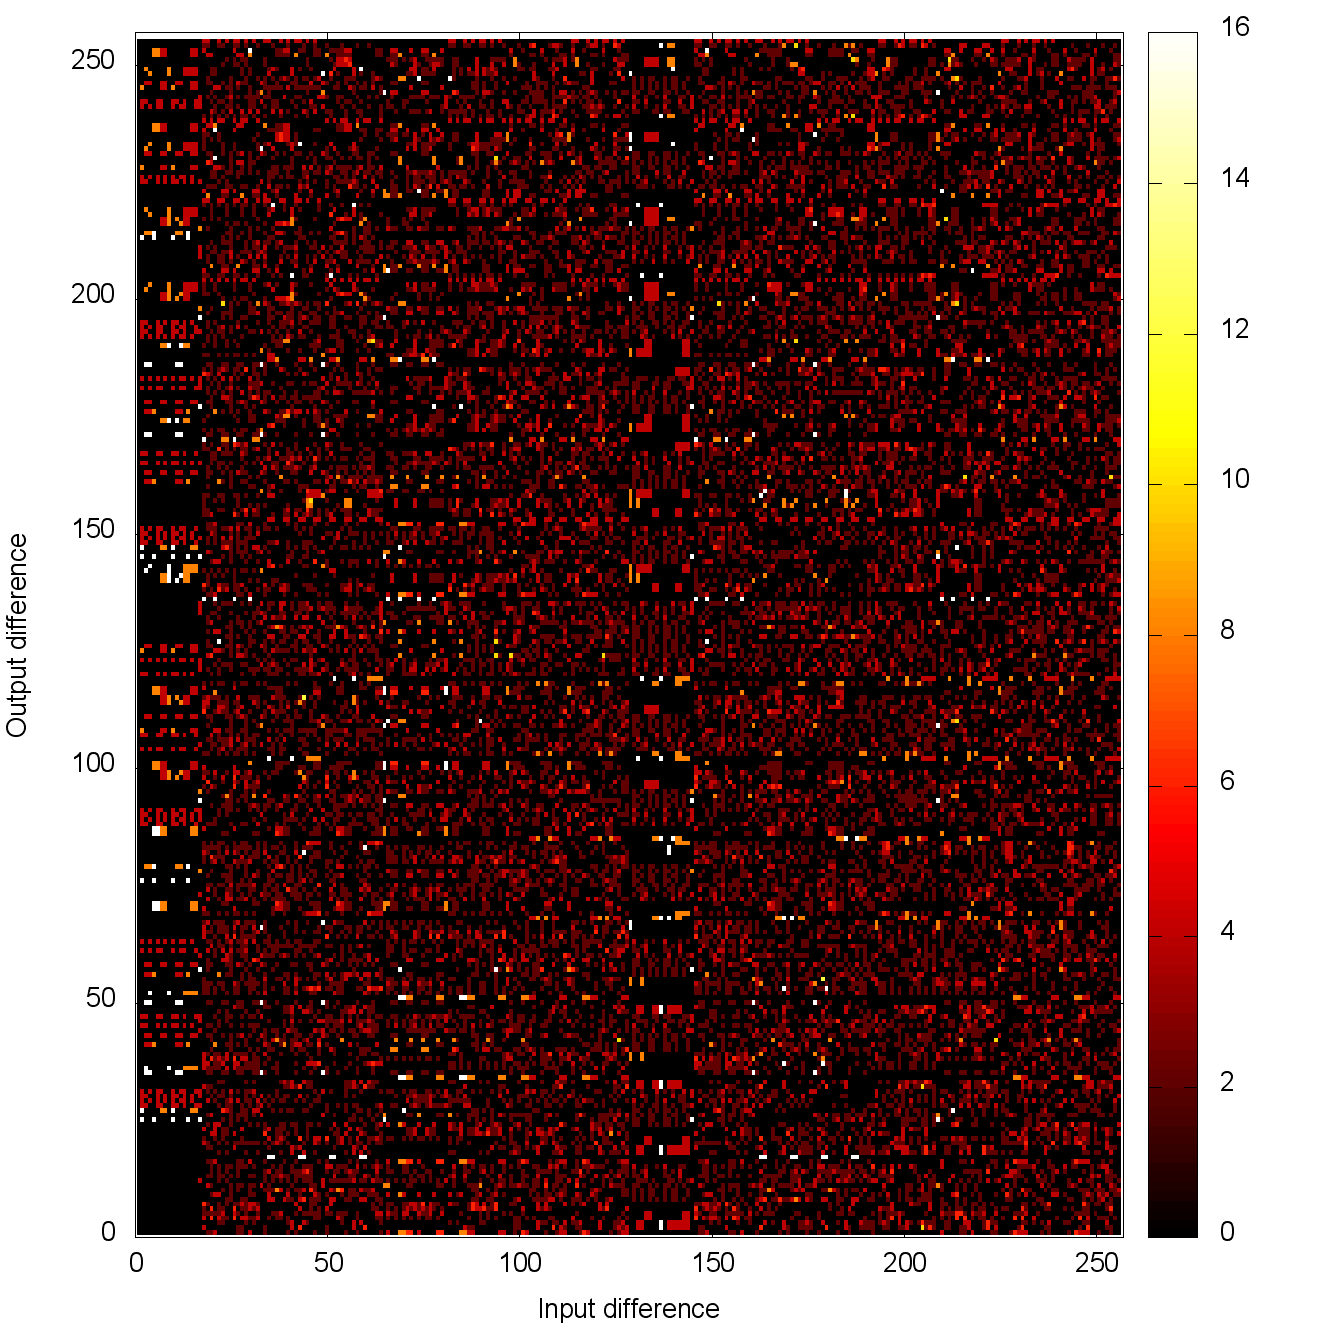
\includegraphics[scale=0.35]{../II_LOTF/littlun/littlun_s1_ddt.png}
\caption{DDT of \littlunOne \label{littDDT}.}
\end{figure}

\begin{figure}[ht]
\centering
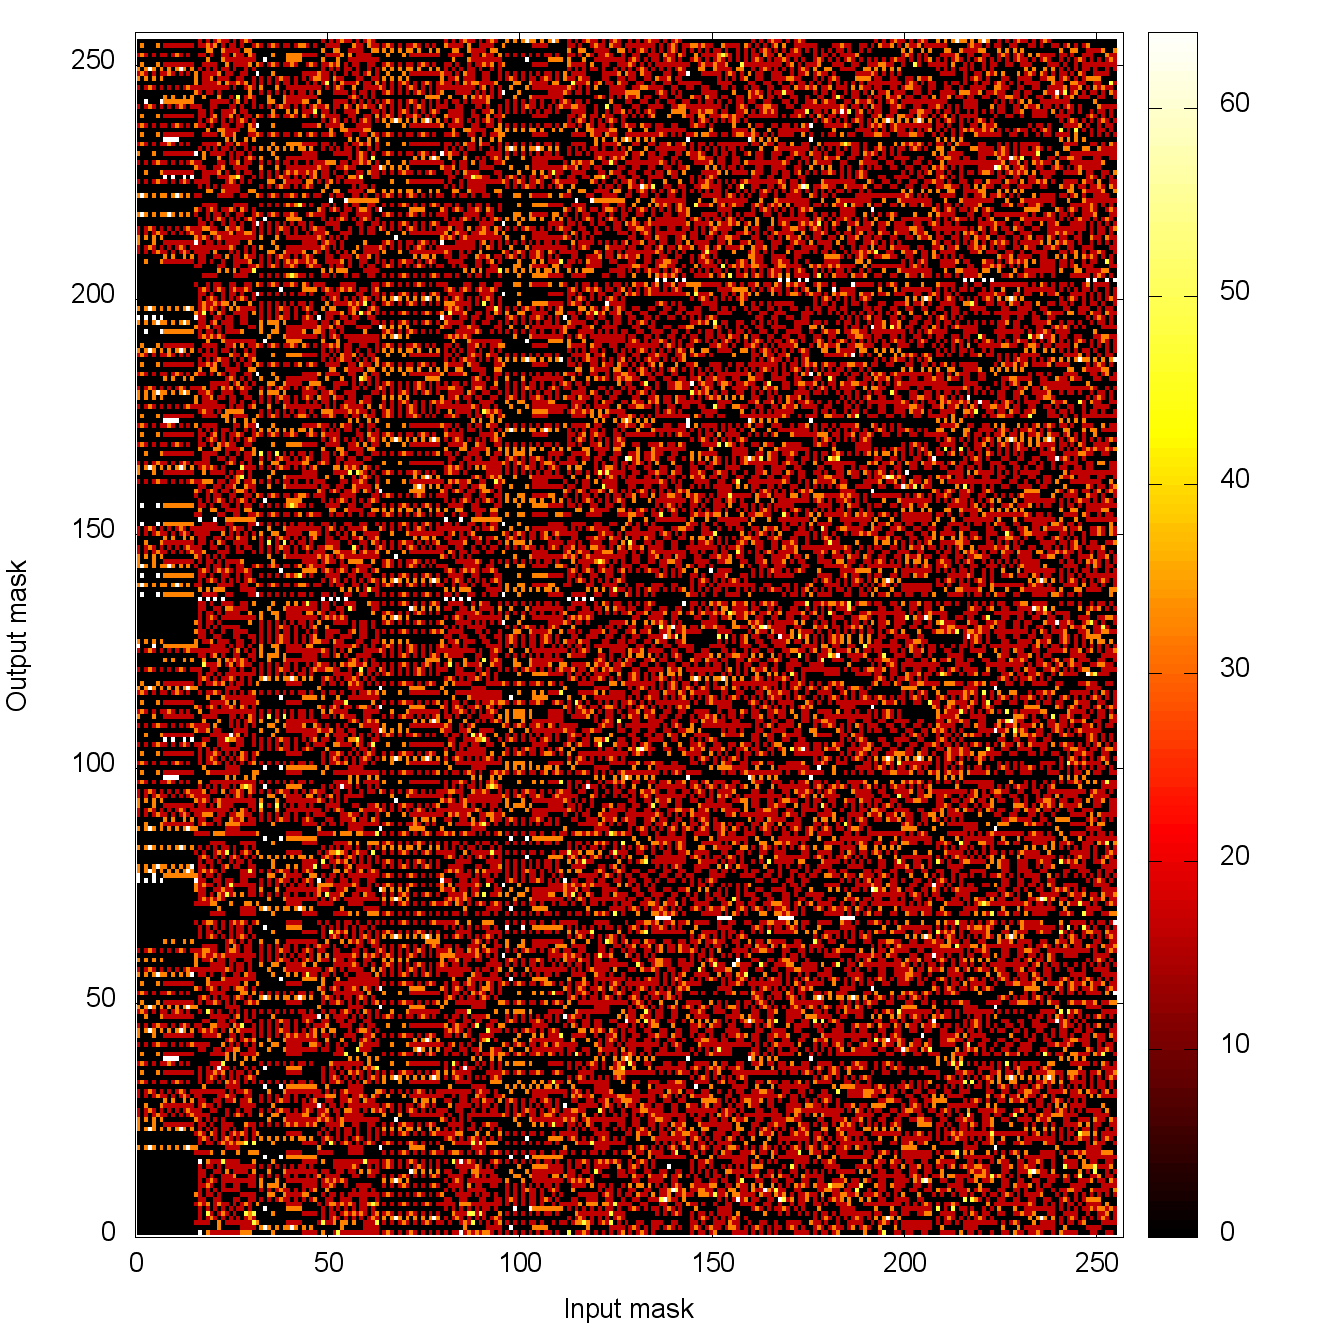
\includegraphics[scale=0.35]{../II_LOTF/littlun/littlun_s1_lat.png}
\caption{LAT of \littlunOne \label{littLAT}.}
\end{figure}

% That one's incorrect (old S-box)
%
%\begin{table}[ht]
%\caption{ANF of \littlunOne \label{littANF}}
%			\littlunOne $\Phi_0$:
%			$
%			x_{0} x_{1} x_{3} + x_{0} x_{2} x_{3} x_{7} + x_{0} x_{2} + x_{0} x_{3}
%			x_{5} + x_{0} x_{3} x_{6} x_{7} + x_{0} x_{3} x_{7} + x_{0} x_{3} +
%			x_{1} x_{2} x_{6} + x_{1} x_{2} + x_{1} x_{3} x_{4} + x_{1} + x_{2}
%			x_{3} x_{4} x_{7} + x_{2} x_{3} + x_{2} x_{4} + x_{2} x_{5} x_{6} +
%			x_{2} x_{5} + x_{3} x_{4} x_{5} + x_{3} x_{4} x_{6} x_{7} + x_{3} x_{4}
%			x_{7} + x_{3} x_{4} + x_{3} x_{7} + x_{6}$
%			
%			\littlunOne $\Phi_1$:
%			$
%			x_{0} x_{1} x_{2} x_{3} x_{7} + x_{0} x_{1} x_{2} x_{3} + x_{0} x_{1}
%			x_{3} x_{5} + x_{0} x_{1} x_{3} x_{6} x_{7} + x_{0} x_{1} x_{3} x_{6} +
%			x_{0} x_{1} x_{3} x_{7} + x_{0} x_{1} x_{6} + x_{0} x_{1} x_{7} + x_{0}
%			x_{2} x_{3} x_{5} + x_{0} x_{2} x_{3} + x_{0} x_{2} x_{5} + x_{0} x_{2}
%			x_{6} + x_{0} x_{2} + x_{0} x_{3} x_{5} x_{6} + x_{0} x_{3} x_{5} +
%			x_{0} x_{3} x_{6} x_{7} + x_{0} x_{3} x_{7} + x_{0} x_{3} + x_{0} x_{4}
%			+ x_{0} x_{5} x_{6} + x_{0} x_{6} x_{7} + x_{0} x_{7} + x_{0} + x_{1}
%			x_{2} x_{3} x_{4} x_{7} + x_{1} x_{2} x_{3} x_{4} + x_{1} x_{2} x_{3}
%			x_{5} + x_{1} x_{2} x_{3} x_{6} x_{7} + x_{1} x_{2} x_{3} x_{6} + x_{1}
%			x_{2} x_{3} x_{7} + x_{1} x_{2} x_{3} + x_{1} x_{2} x_{4} + x_{1} x_{2}
%			x_{5} x_{6} + x_{1} x_{2} x_{5} x_{7} + x_{1} x_{2} x_{5} + x_{1} x_{2}
%			x_{6} x_{7} + x_{1} x_{3} x_{4} x_{5} + x_{1} x_{3} x_{4} x_{6} x_{7} +
%			x_{1} x_{3} x_{4} x_{6} + x_{1} x_{3} x_{4} x_{7} + x_{1} x_{3} x_{5}
%			x_{6} + x_{1} x_{3} x_{6} + x_{1} x_{3} x_{7} + x_{1} x_{3} + x_{1}
%			x_{4} x_{7} + x_{1} x_{5} x_{6} x_{7} + x_{1} x_{6} x_{7} + x_{1} x_{6}
%			+ x_{1} x_{7} + x_{1} + x_{2} x_{3} x_{4} x_{5} + x_{2} x_{3} x_{4} +
%			x_{2} x_{3} x_{5} x_{6} x_{7} + x_{2} x_{3} x_{5} x_{6} + x_{2} x_{3}
%			x_{5} x_{7} + x_{2} x_{3} x_{5} + x_{2} x_{3} x_{6} + x_{2} x_{3} x_{7}
%			+ x_{2} x_{4} x_{6} + x_{2} x_{4} + x_{2} x_{5} x_{6} x_{7} + x_{2}
%			x_{5} x_{6} + x_{2} x_{5} x_{7} + x_{2} x_{6} + x_{2} x_{7} + x_{2} +
%			x_{3} x_{4} x_{5} x_{6} + x_{3} x_{4} x_{5} + x_{3} x_{4} x_{6} x_{7} +
%			x_{3} x_{4} x_{7} + x_{3} x_{5} + x_{3} x_{6} + x_{4} x_{6} x_{7} +
%			x_{4} x_{7} + x_{4} + x_{5} x_{6} + x_{5} + x_{6} + x_{7}$
%			
%			\littlunOne $\Phi_2$:
%			$
%			x_{0} x_{1} x_{2} x_{6} + x_{0} x_{1} x_{3} x_{4} + x_{0} x_{1} + x_{0}
%			x_{2} x_{3} x_{4} x_{7} + x_{0} x_{2} x_{3} x_{6} + x_{0} x_{2} x_{3} +
%			x_{0} x_{2} x_{4} + x_{0} x_{2} x_{5} x_{6} + x_{0} x_{2} x_{6} x_{7} +
%			x_{0} x_{2} x_{6} + x_{0} x_{3} x_{4} x_{5} + x_{0} x_{3} x_{4} x_{6}
%			x_{7} + x_{0} x_{3} x_{4} x_{7} + x_{0} x_{3} x_{4} + x_{0} x_{3} x_{7}
%			+ x_{0} x_{6} + x_{0} + x_{1} x_{2} x_{4} + x_{1} x_{2} x_{7} + x_{1}
%			x_{3} x_{4} + x_{1} x_{3} x_{6} + x_{1} x_{3} x_{7} + x_{1} x_{3} +
%			x_{1} x_{5} + x_{1} x_{6} x_{7} + x_{1} x_{6} + x_{1} x_{7} + x_{1} +
%			x_{2} x_{3} x_{4} x_{6} + x_{2} x_{3} x_{4} x_{7} + x_{2} x_{3} x_{5} +
%			x_{2} x_{3} x_{6} x_{7} + x_{2} x_{3} x_{6} + x_{2} x_{3} x_{7} + x_{2}
%			x_{3} + x_{2} x_{4} x_{5} + x_{2} x_{4} x_{6} x_{7} + x_{2} x_{4} x_{6}
%			+ x_{2} x_{4} + x_{2} x_{5} + x_{2} x_{6} x_{7} + x_{2} x_{6} + x_{3}
%			x_{4} x_{5} + x_{3} x_{4} x_{6} x_{7} + x_{3} x_{4} x_{7} + x_{3} x_{4}
%			+ x_{3} x_{5} x_{7} + x_{3} x_{6} x_{7} + x_{3} + x_{4} + x_{6} $
%			
%			\littlunOne $\Phi_3$:
%			$
%			x_{0} x_{1} x_{2} x_{3} + x_{0} x_{1} x_{2} x_{7} + x_{0} x_{1} x_{3}
%			x_{6} + x_{0} x_{1} x_{3} + x_{0} x_{1} x_{5} + x_{0} x_{1} x_{6} x_{7}
%			+ x_{0} x_{1} x_{7} + x_{0} x_{2} x_{5} + x_{0} x_{2} + x_{0} x_{3}
%			x_{6} + x_{0} x_{3} + x_{0} x_{5} x_{6} + x_{0} x_{5} + x_{0} x_{6}
%			x_{7} + x_{0} x_{7} + x_{0} + x_{1} x_{2} x_{3} x_{4} + x_{1} x_{2}
%			x_{3} x_{6} + x_{1} x_{2} x_{3} + x_{1} x_{2} x_{4} x_{7} + x_{1} x_{2}
%			x_{6} x_{7} + x_{1} x_{2} x_{6} + x_{1} x_{2} x_{7} + x_{1} x_{3} x_{4}
%			x_{6} + x_{1} x_{3} x_{4} + x_{1} x_{3} + x_{1} x_{4} x_{5} + x_{1}
%			x_{4} x_{6} x_{7} + x_{1} x_{4} x_{7} + x_{1} x_{7} + x_{1} + x_{2}
%			x_{3} x_{5} x_{6} + x_{2} x_{3} x_{5} + x_{2} x_{3} + x_{2} x_{4} x_{5}
%			+ x_{2} x_{4} + x_{2} x_{5} x_{6} x_{7} + x_{2} x_{5} x_{6} + x_{2}
%			x_{5} x_{7} + x_{2} x_{5} + x_{2} x_{6} + x_{2} x_{7} + x_{3} x_{4}
%			x_{6} + x_{3} x_{4} + x_{4} x_{5} x_{6} + x_{4} x_{5} + x_{4} x_{6}
%			x_{7} + x_{4} x_{7} + x_{5} + x_{6}$
%			
%			\littlunOne $\Phi_4$:
%			$
%			x_{0} x_{1} x_{7} + x_{0} x_{2} x_{3} x_{7} + x_{0} x_{3} x_{6} x_{7} +
%			x_{0} x_{3} x_{7} + x_{0} x_{5} x_{7} + x_{0} x_{6} + x_{0} x_{7} +
%			x_{1} x_{2} x_{6} + x_{1} x_{4} x_{7} + x_{1} x_{6} + x_{2} x_{3} x_{4}
%			x_{7} + x_{2} x_{5} x_{6} + x_{2} + x_{3} x_{4} x_{6} x_{7} + x_{3}
%			x_{4} x_{7} + x_{3} x_{7} + x_{4} x_{5} x_{7} + x_{4} x_{6} + x_{4}
%			x_{7} + x_{5} x_{6} + x_{5} + x_{6} x_{7}$
%			
%			\littlunOne $\Phi_5$:
%			$
%			x_{0} x_{1} x_{2} x_{7} + x_{0} x_{1} x_{5} x_{7} + x_{0} x_{1} x_{6}
%			x_{7} + x_{0} x_{1} x_{7} + x_{0} x_{2} x_{3} x_{5} x_{7} + x_{0} x_{2}
%			x_{3} x_{7} + x_{0} x_{2} x_{3} + x_{0} x_{2} x_{5} x_{7} + x_{0} x_{2}
%			x_{6} + x_{0} x_{3} x_{5} x_{6} x_{7} + x_{0} x_{3} x_{5} x_{7} + x_{0}
%			x_{3} x_{5} + x_{0} x_{3} x_{7} + x_{0} x_{3} + x_{0} x_{4} + x_{0}
%			x_{5} x_{6} x_{7} + x_{0} x_{5} x_{6} + x_{0} x_{6} x_{7} + x_{0} x_{6}
%			+ x_{0} + x_{1} x_{2} x_{3} x_{5} + x_{1} x_{2} x_{3} x_{6} x_{7} +
%			x_{1} x_{2} x_{3} x_{6} + x_{1} x_{2} x_{4} x_{7} + x_{1} x_{2} x_{4} +
%			x_{1} x_{2} x_{5} x_{6} + x_{1} x_{2} x_{5} x_{7} + x_{1} x_{2} x_{6}
%			x_{7} + x_{1} x_{2} x_{6} + x_{1} x_{2} + x_{1} x_{3} x_{5} x_{6} +
%			x_{1} x_{3} x_{6} x_{7} + x_{1} x_{3} x_{6} + x_{1} x_{4} x_{5} x_{7} +
%			x_{1} x_{4} x_{6} x_{7} + x_{1} x_{4} x_{6} + x_{1} x_{4} x_{7} + x_{1}
%			x_{5} x_{6} x_{7} + x_{1} x_{5} x_{6} + x_{1} x_{6} x_{7} + x_{1} x_{7}
%			+ x_{1} + x_{2} x_{3} x_{4} x_{5} x_{7} + x_{2} x_{3} x_{4} x_{7} +
%			x_{2} x_{3} x_{4} + x_{2} x_{3} x_{5} x_{6} x_{7} + x_{2} x_{3} x_{5}
%			x_{6} + x_{2} x_{3} x_{5} + x_{2} x_{4} x_{5} x_{7} + x_{2} x_{4} x_{5}
%			+ x_{2} x_{4} x_{6} + x_{2} x_{5} x_{6} x_{7} + x_{2} x_{5} x_{7} +
%			x_{2} x_{5} + x_{2} x_{6} x_{7} + x_{2} x_{6} + x_{2} x_{7} + x_{2} +
%			x_{3} x_{4} x_{5} x_{6} x_{7} + x_{3} x_{4} x_{5} x_{7} + x_{3} x_{4}
%			x_{5} + x_{3} x_{4} x_{7} + x_{3} x_{4} + x_{3} x_{5} x_{6} x_{7} +
%			x_{3} x_{5} x_{7} + x_{3} x_{5} + x_{3} x_{6} x_{7} + x_{3} x_{6} +
%			x_{3} + x_{4} x_{5} x_{6} x_{7} + x_{4} x_{6} x_{7} + x_{4} x_{6} +
%			x_{4} x_{7} + x_{4} + x_{5} x_{6} x_{7} + x_{5} x_{7} + x_{5} + x_{6}
%			$
%			
%			\littlunOne $\Phi_6$:
%			$
%			x_{0} x_{1} x_{4} x_{7} + x_{0} x_{1} x_{6} + x_{0} x_{1} x_{7} + x_{0}
%			x_{2} x_{3} x_{4} x_{7} + x_{0} x_{2} x_{3} x_{6} + x_{0} x_{2} x_{3}
%			x_{7} + x_{0} x_{2} x_{6} x_{7} + x_{0} x_{2} x_{6} + x_{0} x_{3} x_{4}
%			x_{6} x_{7} + x_{0} x_{3} x_{4} x_{7} + x_{0} x_{3} x_{6} x_{7} + x_{0}
%			x_{3} x_{7} + x_{0} x_{4} x_{5} x_{7} + x_{0} x_{4} x_{6} + x_{0} x_{4}
%			x_{7} + x_{0} x_{5} x_{6} + x_{0} x_{5} x_{7} + x_{0} x_{6} + x_{0}
%			x_{7} + x_{0} + x_{1} x_{2} x_{4} x_{6} + x_{1} x_{3} x_{7} + x_{1}
%			x_{5} + x_{1} x_{6} x_{7} + x_{1} x_{6} + x_{2} x_{3} x_{4} x_{6} +
%			x_{2} x_{3} x_{5} + x_{2} x_{3} x_{6} x_{7} + x_{2} x_{3} x_{6} + x_{2}
%			x_{3} x_{7} + x_{2} x_{4} x_{5} x_{6} + x_{2} x_{4} x_{6} x_{7} + x_{2}
%			x_{4} x_{6} + x_{2} x_{4} + x_{2} x_{5} x_{7} + x_{2} x_{5} + x_{2}
%			x_{6} x_{7} + x_{2} x_{6} + x_{2} + x_{3} x_{4} x_{7} + x_{3} x_{5}
%			x_{6} + x_{3} x_{5} x_{7} + x_{3} x_{5} + x_{3} x_{6} x_{7} + x_{4}
%			x_{5} + x_{4} x_{6} x_{7} + x_{4} + x_{5} x_{7} + x_{5} + x_{6} x_{7} +
%			x_{7}$
%			
%			\littlunOne $\Phi_7:$
%			$
%			x_{0} x_{1} x_{2} + x_{0} x_{1} x_{5} + x_{0} x_{1} x_{6} + x_{0} x_{1}
%			+ x_{0} x_{2} x_{3} x_{5} + x_{0} x_{2} x_{3} + x_{0} x_{2} x_{5} x_{7}
%			+ x_{0} x_{2} x_{7} + x_{0} x_{3} x_{5} x_{6} + x_{0} x_{3} x_{5} +
%			x_{0} x_{3} + x_{0} x_{5} x_{6} x_{7} + x_{0} x_{5} x_{7} + x_{0} x_{6}
%			+ x_{0} x_{7} + x_{1} x_{2} x_{3} x_{6} + x_{1} x_{2} x_{4} + x_{1}
%			x_{2} x_{6} x_{7} + x_{1} x_{2} x_{6} + x_{1} x_{3} x_{6} + x_{1} x_{4}
%			x_{5} + x_{1} x_{4} x_{6} + x_{1} x_{4} + x_{1} x_{6} x_{7} + x_{1}
%			x_{6} + x_{1} + x_{2} x_{3} x_{4} x_{5} + x_{2} x_{3} x_{4} + x_{2}
%			x_{3} x_{5} x_{6} + x_{2} x_{4} x_{5} x_{7} + x_{2} x_{4} x_{7} + x_{2}
%			x_{5} x_{6} x_{7} + x_{2} x_{5} x_{6} + x_{2} x_{6} + x_{2} + x_{3}
%			x_{4} x_{5} x_{6} + x_{3} x_{4} x_{5} + x_{3} x_{4} + x_{3} x_{5} x_{6}
%			+ x_{3} x_{5} + x_{3} x_{6} + x_{4} x_{5} x_{6} x_{7} + x_{4} x_{5}
%			x_{7} + x_{4} x_{6} + x_{4} x_{7} + x_{4} + x_{5} x_{6} x_{7} + x_{5}
%			x_{7} + x_{5} + x_{6} x_{7}$
%\end{table}
%
%\begin{table}[ht]
%\caption{ANF of the inverse of \littlunOne \label{littInvANF}}
%$\littlunOne^{-1}$ $\Phi_0$:
%$
%x_{0} x_{1} x_{3} + x_{0} x_{2} x_{3} x_{7} + x_{0} x_{2} + x_{0} x_{3}
%x_{5} + x_{0} x_{3} x_{6} x_{7} + x_{0} x_{3} x_{7} + x_{0} x_{3} +
%x_{1} x_{2} x_{6} + x_{1} x_{2} + x_{1} x_{3} x_{4} + x_{1} + x_{2}
%x_{3} x_{4} x_{7} + x_{2} x_{3} + x_{2} x_{4} + x_{2} x_{5} x_{6} +
%x_{2} x_{5} + x_{3} x_{4} x_{5} + x_{3} x_{4} x_{6} x_{7} + x_{3} x_{4}
%x_{7} + x_{3} x_{4} + x_{3} x_{7} + x_{6}
%$
%
%$\littlunOne^{-1}$ $\Phi_1$:
%$
%x_{0} x_{1} x_{2} x_{3} x_{7} + x_{0} x_{1} x_{2} x_{3} + x_{0} x_{1}
%x_{3} x_{5} + x_{0} x_{1} x_{3} x_{6} x_{7} + x_{0} x_{1} x_{3} x_{6} +
%x_{0} x_{1} x_{3} x_{7} + x_{0} x_{1} x_{6} + x_{0} x_{1} x_{7} + x_{0}
%x_{2} x_{3} x_{5} + x_{0} x_{2} x_{3} + x_{0} x_{2} x_{5} + x_{0} x_{2}
%x_{6} + x_{0} x_{2} + x_{0} x_{3} x_{5} x_{6} + x_{0} x_{3} x_{5} +
%x_{0} x_{3} x_{6} x_{7} + x_{0} x_{3} x_{7} + x_{0} x_{3} + x_{0} x_{4}
%+ x_{0} x_{5} x_{6} + x_{0} x_{6} x_{7} + x_{0} x_{7} + x_{0} + x_{1}
%x_{2} x_{3} x_{4} x_{7} + x_{1} x_{2} x_{3} x_{4} + x_{1} x_{2} x_{3}
%x_{5} + x_{1} x_{2} x_{3} x_{6} x_{7} + x_{1} x_{2} x_{3} x_{6} + x_{1}
%x_{2} x_{3} x_{7} + x_{1} x_{2} x_{3} + x_{1} x_{2} x_{4} + x_{1} x_{2}
%x_{5} x_{6} + x_{1} x_{2} x_{5} x_{7} + x_{1} x_{2} x_{5} + x_{1} x_{2}
%x_{6} x_{7} + x_{1} x_{3} x_{4} x_{5} + x_{1} x_{3} x_{4} x_{6} x_{7} +
%x_{1} x_{3} x_{4} x_{6} + x_{1} x_{3} x_{4} x_{7} + x_{1} x_{3} x_{5}
%x_{6} + x_{1} x_{3} x_{6} + x_{1} x_{3} x_{7} + x_{1} x_{3} + x_{1}
%x_{4} x_{7} + x_{1} x_{5} x_{6} x_{7} + x_{1} x_{6} x_{7} + x_{1} x_{6}
%+ x_{1} x_{7} + x_{1} + x_{2} x_{3} x_{4} x_{5} + x_{2} x_{3} x_{4} +
%x_{2} x_{3} x_{5} x_{6} x_{7} + x_{2} x_{3} x_{5} x_{6} + x_{2} x_{3}
%x_{5} x_{7} + x_{2} x_{3} x_{5} + x_{2} x_{3} x_{6} + x_{2} x_{3} x_{7}
%+ x_{2} x_{4} x_{6} + x_{2} x_{4} + x_{2} x_{5} x_{6} x_{7} + x_{2}
%x_{5} x_{6} + x_{2} x_{5} x_{7} + x_{2} x_{6} + x_{2} x_{7} + x_{2} +
%x_{3} x_{4} x_{5} x_{6} + x_{3} x_{4} x_{5} + x_{3} x_{4} x_{6} x_{7} +
%x_{3} x_{4} x_{7} + x_{3} x_{5} + x_{3} x_{6} + x_{4} x_{6} x_{7} +
%x_{4} x_{7} + x_{4} + x_{5} x_{6} + x_{5} + x_{6} + x_{7}
%$
%
%$\littlunOne^{-1}$ $\Phi_2$:
%$
%x_{0} x_{1} x_{2} x_{6} + x_{0} x_{1} x_{3} x_{4} + x_{0} x_{1} + x_{0}
%x_{2} x_{3} x_{4} x_{7} + x_{0} x_{2} x_{3} x_{6} + x_{0} x_{2} x_{3} +
%x_{0} x_{2} x_{4} + x_{0} x_{2} x_{5} x_{6} + x_{0} x_{2} x_{6} x_{7} +
%x_{0} x_{2} x_{6} + x_{0} x_{3} x_{4} x_{5} + x_{0} x_{3} x_{4} x_{6}
%x_{7} + x_{0} x_{3} x_{4} x_{7} + x_{0} x_{3} x_{4} + x_{0} x_{3} x_{7}
%+ x_{0} x_{6} + x_{0} + x_{1} x_{2} x_{4} + x_{1} x_{2} x_{7} + x_{1}
%x_{3} x_{4} + x_{1} x_{3} x_{6} + x_{1} x_{3} x_{7} + x_{1} x_{3} +
%x_{1} x_{5} + x_{1} x_{6} x_{7} + x_{1} x_{6} + x_{1} x_{7} + x_{1} +
%x_{2} x_{3} x_{4} x_{6} + x_{2} x_{3} x_{4} x_{7} + x_{2} x_{3} x_{5} +
%x_{2} x_{3} x_{6} x_{7} + x_{2} x_{3} x_{6} + x_{2} x_{3} x_{7} + x_{2}
%x_{3} + x_{2} x_{4} x_{5} + x_{2} x_{4} x_{6} x_{7} + x_{2} x_{4} x_{6}
%+ x_{2} x_{4} + x_{2} x_{5} + x_{2} x_{6} x_{7} + x_{2} x_{6} + x_{3}
%x_{4} x_{5} + x_{3} x_{4} x_{6} x_{7} + x_{3} x_{4} x_{7} + x_{3} x_{4}
%+ x_{3} x_{5} x_{7} + x_{3} x_{6} x_{7} + x_{3} + x_{4} + x_{6}
%$
%
%$\littlunOne^{-1}$ $\Phi_3$:
%$
%x_{0} x_{1} x_{2} x_{3} + x_{0} x_{1} x_{2} x_{7} + x_{0} x_{1} x_{3}
%x_{6} + x_{0} x_{1} x_{3} + x_{0} x_{1} x_{5} + x_{0} x_{1} x_{6} x_{7}
%+ x_{0} x_{1} x_{7} + x_{0} x_{2} x_{5} + x_{0} x_{2} + x_{0} x_{3}
%x_{6} + x_{0} x_{3} + x_{0} x_{5} x_{6} + x_{0} x_{5} + x_{0} x_{6}
%x_{7} + x_{0} x_{7} + x_{0} + x_{1} x_{2} x_{3} x_{4} + x_{1} x_{2}
%x_{3} x_{6} + x_{1} x_{2} x_{3} + x_{1} x_{2} x_{4} x_{7} + x_{1} x_{2}
%x_{6} x_{7} + x_{1} x_{2} x_{6} + x_{1} x_{2} x_{7} + x_{1} x_{3} x_{4}
%x_{6} + x_{1} x_{3} x_{4} + x_{1} x_{3} + x_{1} x_{4} x_{5} + x_{1}
%x_{4} x_{6} x_{7} + x_{1} x_{4} x_{7} + x_{1} x_{7} + x_{1} + x_{2}
%x_{3} x_{5} x_{6} + x_{2} x_{3} x_{5} + x_{2} x_{3} + x_{2} x_{4} x_{5}
%+ x_{2} x_{4} + x_{2} x_{5} x_{6} x_{7} + x_{2} x_{5} x_{6} + x_{2}
%x_{5} x_{7} + x_{2} x_{5} + x_{2} x_{6} + x_{2} x_{7} + x_{3} x_{4}
%x_{6} + x_{3} x_{4} + x_{4} x_{5} x_{6} + x_{4} x_{5} + x_{4} x_{6}
%x_{7} + x_{4} x_{7} + x_{5} + x_{6}
%$
%
%$\littlunOne^{-1}$ $\Phi_4$:
%$
%x_{0} x_{1} x_{7} + x_{0} x_{2} x_{3} x_{7} + x_{0} x_{3} x_{6} x_{7} +
%x_{0} x_{3} x_{7} + x_{0} x_{5} x_{7} + x_{0} x_{6} + x_{0} x_{7} +
%x_{1} x_{2} x_{6} + x_{1} x_{4} x_{7} + x_{1} x_{6} + x_{2} x_{3} x_{4}
%x_{7} + x_{2} x_{5} x_{6} + x_{2} + x_{3} x_{4} x_{6} x_{7} + x_{3}
%x_{4} x_{7} + x_{3} x_{7} + x_{4} x_{5} x_{7} + x_{4} x_{6} + x_{4}
%x_{7} + x_{5} x_{6} + x_{5} + x_{6} x_{7}
%$
%
%$\littlunOne^{-1}$ $\Phi_5$:
%$
%x_{0} x_{1} x_{2} x_{7} + x_{0} x_{1} x_{5} x_{7} + x_{0} x_{1} x_{6}
%x_{7} + x_{0} x_{1} x_{7} + x_{0} x_{2} x_{3} x_{5} x_{7} + x_{0} x_{2}
%x_{3} x_{7} + x_{0} x_{2} x_{3} + x_{0} x_{2} x_{5} x_{7} + x_{0} x_{2}
%x_{6} + x_{0} x_{3} x_{5} x_{6} x_{7} + x_{0} x_{3} x_{5} x_{7} + x_{0}
%x_{3} x_{5} + x_{0} x_{3} x_{7} + x_{0} x_{3} + x_{0} x_{4} + x_{0}
%x_{5} x_{6} x_{7} + x_{0} x_{5} x_{6} + x_{0} x_{6} x_{7} + x_{0} x_{6}
%+ x_{0} + x_{1} x_{2} x_{3} x_{5} + x_{1} x_{2} x_{3} x_{6} x_{7} +
%x_{1} x_{2} x_{3} x_{6} + x_{1} x_{2} x_{4} x_{7} + x_{1} x_{2} x_{4} +
%x_{1} x_{2} x_{5} x_{6} + x_{1} x_{2} x_{5} x_{7} + x_{1} x_{2} x_{6}
%x_{7} + x_{1} x_{2} x_{6} + x_{1} x_{2} + x_{1} x_{3} x_{5} x_{6} +
%x_{1} x_{3} x_{6} x_{7} + x_{1} x_{3} x_{6} + x_{1} x_{4} x_{5} x_{7} +
%x_{1} x_{4} x_{6} x_{7} + x_{1} x_{4} x_{6} + x_{1} x_{4} x_{7} + x_{1}
%x_{5} x_{6} x_{7} + x_{1} x_{5} x_{6} + x_{1} x_{6} x_{7} + x_{1} x_{7}
%+ x_{1} + x_{2} x_{3} x_{4} x_{5} x_{7} + x_{2} x_{3} x_{4} x_{7} +
%x_{2} x_{3} x_{4} + x_{2} x_{3} x_{5} x_{6} x_{7} + x_{2} x_{3} x_{5}
%x_{6} + x_{2} x_{3} x_{5} + x_{2} x_{4} x_{5} x_{7} + x_{2} x_{4} x_{5}
%+ x_{2} x_{4} x_{6} + x_{2} x_{5} x_{6} x_{7} + x_{2} x_{5} x_{7} +
%x_{2} x_{5} + x_{2} x_{6} x_{7} + x_{2} x_{6} + x_{2} x_{7} + x_{2} +
%x_{3} x_{4} x_{5} x_{6} x_{7} + x_{3} x_{4} x_{5} x_{7} + x_{3} x_{4}
%x_{5} + x_{3} x_{4} x_{7} + x_{3} x_{4} + x_{3} x_{5} x_{6} x_{7} +
%x_{3} x_{5} x_{7} + x_{3} x_{5} + x_{3} x_{6} x_{7} + x_{3} x_{6} +
%x_{3} + x_{4} x_{5} x_{6} x_{7} + x_{4} x_{6} x_{7} + x_{4} x_{6} +
%x_{4} x_{7} + x_{4} + x_{5} x_{6} x_{7} + x_{5} x_{7} + x_{5} + x_{6}
%$
%
%$\littlunOne^{-1}$ $\Phi_6$:
%$
%x_{0} x_{1} x_{4} x_{7} + x_{0} x_{1} x_{6} + x_{0} x_{1} x_{7} + x_{0}
%x_{2} x_{3} x_{4} x_{7} + x_{0} x_{2} x_{3} x_{6} + x_{0} x_{2} x_{3}
%x_{7} + x_{0} x_{2} x_{6} x_{7} + x_{0} x_{2} x_{6} + x_{0} x_{3} x_{4}
%x_{6} x_{7} + x_{0} x_{3} x_{4} x_{7} + x_{0} x_{3} x_{6} x_{7} + x_{0}
%x_{3} x_{7} + x_{0} x_{4} x_{5} x_{7} + x_{0} x_{4} x_{6} + x_{0} x_{4}
%x_{7} + x_{0} x_{5} x_{6} + x_{0} x_{5} x_{7} + x_{0} x_{6} + x_{0}
%x_{7} + x_{0} + x_{1} x_{2} x_{4} x_{6} + x_{1} x_{3} x_{7} + x_{1}
%x_{5} + x_{1} x_{6} x_{7} + x_{1} x_{6} + x_{2} x_{3} x_{4} x_{6} +
%x_{2} x_{3} x_{5} + x_{2} x_{3} x_{6} x_{7} + x_{2} x_{3} x_{6} + x_{2}
%x_{3} x_{7} + x_{2} x_{4} x_{5} x_{6} + x_{2} x_{4} x_{6} x_{7} + x_{2}
%x_{4} x_{6} + x_{2} x_{4} + x_{2} x_{5} x_{7} + x_{2} x_{5} + x_{2}
%x_{6} x_{7} + x_{2} x_{6} + x_{2} + x_{3} x_{4} x_{7} + x_{3} x_{5}
%x_{6} + x_{3} x_{5} x_{7} + x_{3} x_{5} + x_{3} x_{6} x_{7} + x_{4}
%x_{5} + x_{4} x_{6} x_{7} + x_{4} + x_{5} x_{7} + x_{5} + x_{6} x_{7} +
%x_{7}
%$
%
%$\littlunOne^{-1}$ $\Phi_7$:
%$
%x_{0} x_{1} x_{2} + x_{0} x_{1} x_{5} + x_{0} x_{1} x_{6} + x_{0} x_{1}
%+ x_{0} x_{2} x_{3} x_{5} + x_{0} x_{2} x_{3} + x_{0} x_{2} x_{5} x_{7}
%+ x_{0} x_{2} x_{7} + x_{0} x_{3} x_{5} x_{6} + x_{0} x_{3} x_{5} +
%x_{0} x_{3} + x_{0} x_{5} x_{6} x_{7} + x_{0} x_{5} x_{7} + x_{0} x_{6}
%+ x_{0} x_{7} + x_{1} x_{2} x_{3} x_{6} + x_{1} x_{2} x_{4} + x_{1}
%x_{2} x_{6} x_{7} + x_{1} x_{2} x_{6} + x_{1} x_{3} x_{6} + x_{1} x_{4}
%x_{5} + x_{1} x_{4} x_{6} + x_{1} x_{4} + x_{1} x_{6} x_{7} + x_{1}
%x_{6} + x_{1} + x_{2} x_{3} x_{4} x_{5} + x_{2} x_{3} x_{4} + x_{2}
%x_{3} x_{5} x_{6} + x_{2} x_{4} x_{5} x_{7} + x_{2} x_{4} x_{7} + x_{2}
%x_{5} x_{6} x_{7} + x_{2} x_{5} x_{6} + x_{2} x_{6} + x_{2} + x_{3}
%x_{4} x_{5} x_{6} + x_{3} x_{4} x_{5} + x_{3} x_{4} + x_{3} x_{5} x_{6}
%+ x_{3} x_{5} + x_{3} x_{6} + x_{4} x_{5} x_{6} x_{7} + x_{4} x_{5}
%x_{7} + x_{4} x_{6} + x_{4} x_{7} + x_{4} + x_{5} x_{6} x_{7} + x_{5}
%x_{7} + x_{5} + x_{6} x_{7}
%$
%\end{table}

\FloatBarrier

\section{Examples of implementation of \littlunOne}

\subsection{Tables for \littlunOne and \littlunS}
\label{sec:sbox_tables}

\begin{figure}[ht]
\begin{minted}[breaklines]{c}
uint8_t littlun1_s4[16] =
        {0x0, 0xa, 0x4, 0xf, 0xc, 0x7, 0x2, 0x8,
         0xd, 0xe, 0x9, 0xb, 0x5, 0x6, 0x3, 0x1};
\end{minted}
\caption{The 4-bit S-box \littlunS used in \littlunOne as a \C array\label{tab4}}
\end{figure}

\begin{figure}[ht]
\begin{minted}[breaklines]{c}
uint8_t littlun1[256] =
        {0x00, 0x9b, 0xc2, 0x15, 0x5d, 0x84, 0x4c, 0xd1,
         0x67, 0x38, 0xef, 0xb0, 0x7e, 0x2b, 0xf6, 0xa3,
         0xb9, 0xaa, 0x36, 0x78, 0x2f, 0x6e, 0xe3, 0xf7,
         0x12, 0x5c, 0x9a, 0xd4, 0x89, 0xcd, 0x01, 0x45,
         0x2c, 0x63, 0x44, 0xde, 0x02, 0x96, 0x39, 0x70,
         0xba, 0xe4, 0x18, 0x57, 0xa1, 0xf5, 0x8b, 0xce,
         0x51, 0x87, 0xed, 0xff, 0xb5, 0xa8, 0xca, 0x1b,
         0xdf, 0x90, 0x6c, 0x32, 0x46, 0x03, 0x7d, 0x29,
         0xd5, 0xf2, 0x20, 0x5b, 0xcc, 0x31, 0x04, 0xbd,
         0xa6, 0x41, 0x8e, 0x79, 0xea, 0x9f, 0x68, 0x1c,
         0x48, 0xe6, 0x69, 0x8a, 0x13, 0x77, 0x9e, 0xaf,
         0xf3, 0x05, 0xcb, 0x2d, 0xb4, 0xd0, 0x37, 0x52,
         0xc4, 0x3e, 0x93, 0xac, 0x40, 0xe9, 0x22, 0x56,
         0x7b, 0x8d, 0xf1, 0x06, 0x17, 0x62, 0xbf, 0xda,
         0x1d, 0x7f, 0x07, 0xb1, 0xdb, 0xfa, 0x65, 0x88,
         0x2e, 0xc9, 0xa5, 0x43, 0x58, 0x3c, 0xe0, 0x94,
         0x76, 0x21, 0xab, 0xfd, 0x6a, 0x3f, 0xb7, 0xe2,
         0xdd, 0x4f, 0x53, 0x8c, 0xc0, 0x19, 0x95, 0x08,
         0x83, 0xc5, 0x4e, 0x09, 0x14, 0x50, 0xd8, 0x9c,
         0xf4, 0xee, 0x27, 0x61, 0x3b, 0x7a, 0xa2, 0xb6,
         0xfe, 0xa9, 0x81, 0xc6, 0xe8, 0xbc, 0x1f, 0x5a,
         0x35, 0x72, 0x99, 0x0a, 0xd3, 0x47, 0x24, 0x6d,
         0x0b, 0x4d, 0x75, 0x23, 0x97, 0xd2, 0x60, 0x34,
         0xc8, 0x16, 0xa0, 0xbb, 0xfc, 0xe1, 0x5e, 0x8f,
         0xe7, 0x98, 0x1a, 0x64, 0xae, 0x4b, 0x71, 0x85,
         0x0c, 0xb3, 0x3d, 0xcf, 0x55, 0x28, 0xd9, 0xf0,
         0xb2, 0xdc, 0x5f, 0x30, 0xf9, 0x0d, 0x26, 0xc3,
         0x91, 0xa7, 0x74, 0x1e, 0x82, 0x66, 0x4a, 0xeb,
         0x6f, 0x10, 0xb8, 0xd7, 0x86, 0x73, 0xfb, 0x0e,
         0x59, 0x2a, 0x42, 0xe5, 0x9d, 0xa4, 0x33, 0xc7,
         0x3a, 0x54, 0xec, 0x92, 0xc1, 0x25, 0xad, 0x49,
         0x80, 0x6b, 0xd6, 0xf8, 0x0f, 0xbe, 0x7c, 0x11};
\end{minted}
\caption{The \littlunOne S-box as a \C array\label{tab8}}
\end{figure}

\FloatBarrier

\subsection{SIMD software implementation of \littlunOne}
\label{sec:simdimplem}

In the context of 4 to 8-bit S-boxes, the Lai-Massey structure of the \littlun construction also allows to conveniently use ``vector'' Single Instruction Multiple Data (or SIMD) instructions for
efficient implementations. We discuss here an implementation of \littlunOne based mostly on the \pshufb instruction from Intel's SSSE3 instruction set.
%This instruction
%allows to perform 16 parallel lookups of a 4-bit S-box on a 128-bit register, which is particularly convenient to implement a similarly parallel application of
%a \littlun S-box on 128 bits. More precisely, the semantics of $x' \defas \pshufb~x~y$ can be defined as: 
%\[
%x'[i] \defas \left\{
%				\begin{array}{ll}
%				x[\lfloor y[i]\rfloor_4]  & \text{if the most significant bit of $y[i]$ is not set}\\
%				0 & \text{otherwise}
%				\end{array}
%	    \right.
%\]
%where $x$ and $y$ are vectors of 16 bytes.
The \pshufb instruction can easily be used in an implementation either by directly writing the relevant part of the program in assembler
or by using compiler intrinsics for a language such as \C. In the latter case, the intrinsic corresponding to the use of \pshufb is usually named \texttt{\_mm\_shuffle\_epi8}.
We give a small function implementing the \littlunOne S-box using \C intrinsics in \autoref{sse8}. Even without further tuning of the code, this function compares favourably with vector implementations
of other S-boxes in terms of efficiency. For instance, it needs about half the number of instructions of Hamburg's hand-written vector implementation of the \aes S-box \cite{vpaes}, although
this must be moderated by the fact that the AES S-box is cryptographically stronger.

\begin{figure}[ht]
\begin{minted}[breaklines]{c}
__m128i littlun_ps(__m128i x)
{
  __m128i xlo, xhi, xmid;

  __m128i LO_MASK = _mm_set1_epi8(0x0f);
  __m128i LO_SBOX = _mm_set_epi32(0x01030605, 0x0b090e0d, 0x0802070c, 0x0f040a00);
  __m128i HI_SBOX = _mm_set_epi32(0x10306050, 0xb090e0d0, 0x802070c0, 0xf040a000);

  xhi  = _mm_srli_epi16(x, 4);
  xhi  = _mm_and_si128(xhi, LO_MASK);
  xlo  = _mm_and_si128(x, LO_MASK);
  xmid = _mm_xor_si128(xlo, xhi);

  xmid = _mm_shuffle_epi8(LO_SBOX, xmid);
  xlo  = _mm_xor_si128(xlo, xmid);
  xhi  = _mm_xor_si128(xhi, xmid);

  xlo = _mm_shuffle_epi8(LO_SBOX, xlo);
  xhi = _mm_shuffle_epi8(HI_SBOX, xhi);
  x   = _mm_xor_si128(xlo, xhi);

  return x;
}
\end{minted}
\caption{Snippet for an SSE \C implementation of \littlunOne using compiler intrinsics.\label{sse8}}
\end{figure}

\FloatBarrier

\subsection{Hardware circuit for \littlunS}
\label{sec:circ}

\def\andGate{\begin{tikzpicture}[scale=0.5, circuit logic US]\node [and gate] {};\end{tikzpicture}}
\def\xorGate{\begin{tikzpicture}[scale=0.5, circuit logic US]\node [xor gate] {};\end{tikzpicture}}
\def\orGate{\begin{tikzpicture}[scale=0.5, circuit logic US]\node [or gate] {};\end{tikzpicture}}

\begin{figure}[ht]
\begin{center}
%\begin{turn}{-90}
%\begin{minipage}{4.5cm}
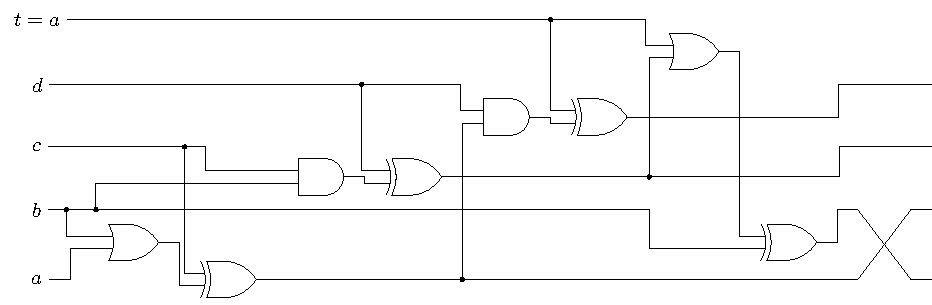
\includegraphics[scale=0.75]{../II_LOTF/littlun/sb4c.pdf}
%\end{minipage}
%\end{turn}
\end{center}
\caption[A circuit implementation of \littlunS.]{A circuit implementation of \littlunS. 
The symbols~\protect\andGate,~\protect\orGate~and~\protect\xorGate~represent the AND,
OR and XOR gates respectively.\label{sb4_circ}}
\end{figure}

\FloatBarrier


\section{AVR implementation of the \fly round function}
\label{sec:mega}

We give pseudo AVR assembly code for the S-box layer, the permutation
and on-the-fly computation of the key-schedule of \fly.
All the state, key and temporary variables fit in the 32 registers of
an ATtiny or ATmega.

\begin{minted}[breaklines]{scheme}
; input/output in s0,...,s7 (with MSBs in s0)
; temporary values held in t0,...,t4
; top XOR
movw t0, s0 ; moves t1:s0 <- s1:s0
movw t2, s2
eor t0, s4
eor t1, s5
eor t2, s6
eor t3, s7
; middle S-box
mov t4, t1
or  t1, t0
eor t1, t2
and t2, t4
eor t2, t3
and t3, t1
eor t3, t0
or  t0, t2
eor t0, t4
; bottom XOR
eor s0, t0
eor s1, t1
eor s2, t2
eor s3, t3
eor s4, t0
eor s5, t1
eor s6, t2
eor s7, t3
; bottom S-boxes
mov t0, s1
or  s1, s0
eor s1, s2
and s2, t0
eor s2, s3
and s3, s1
eor s3, s0
or  s0, s2
eor s0, t0

mov t0, s5
or  s5, s4
eor s5, s6
and s6, t0
eor s6, s7
and s7, s5
eor s7, s4
or  s4, s6
eor s4, t0
\end{minted}
\begin{figure}[ht]
\caption{The \littlunOne S-box on ATmega, using 41 instructions.\label{fig:avrS}}
\end{figure}

\begin{figure}[ht]
\begin{minted}[breaklines]{scheme}
; input/output in s0,...,s7
rol s1
rol s2
rol s2
swap s3
ror s3
swap s4
swap s5
rol s5
ror s6
ror s6
ror s7
\end{minted}
\caption{The $\rot$ permutation on ATmega/ATtiny, using 11 instructions.\label{fig:avrP}}
\end{figure}

\begin{figure}[ht]
\begin{minted}[breaklines]{scheme}
; key input in k0,...,k15
; cipher state in s0,...,s7
; round constant in c0
; temporary register in t0

; add the current round key & round constant to the state
eor s0, k0
eor s1, k1
eor s2, k2
eor s3, k3
eor s4, k4
eor s5, k5
eor s6, k6
eor s7, k7

eor s0, c0
eor s1, 255

; update k0,...,k7 to the next round key
eor k0, k8
eor k1, k9
eor k2, k10
eor k3, k11
eor k4, k12
eor k5, k13
eor k6, k14
eor k7, k15

; update c0 to the next round constant
mov  t0, c0
andi t0, 1
dec  t0
andi t0, 177
lsr  c0
eor  c0, t0
\end{minted}
\caption{Key addition, and the $\ksOne$ key-schedule on ATmega/ATtiny, using 24 instructions.\label{fig:avrK}}
\end{figure}

\FloatBarrier

\FloatBarrier

\section{Hardware implementation of \fly}
\label{implem:hw}
\fly was not designed to be particularly efficient in hardware, and there are clearly better alternatives in that setting. Thus we did not implement \fly in hardware, but it might be informative to very roughly estimate the cost (in GE) of such
an implementation. This can be done by looking at the cost of \present, given the similarity of their structures.
A round-based ASIC implementation of \present-128 can be done for 1884~GE \cite{poschmann}, of which $27\times16$ are dedicated to implementing the 16 S-boxes. If we make the assumption that the key-schedule of \fly does not use significantly more area
than the one of \present-128, we can estimate that a similar round-based implementation of \fly would cost in the area of $1884 - 27\times16 + 80\times8 = 2092$~GE, meaning that the overhead is about
11\,\%.


\section{Test vectors for \fly}
%\color{red}TO UPDATE!!

All numbers are given in big endian (\ie, those are arrays of bytes, with the byte of lowest address on the left).

\medskip

\noindent
\verb+k0: 0x0000000000000000 k1: 0x0000000000000000+

\noindent
\verb+p : 0x0000000000000000+

\noindent
\verb+FLY(k0||k1,p)            : 0x40A942D3FB302724+
 
\medskip

\noindent
\verb+k0: 0x0001020304050607 k1: 0x08090A0B0C0D0E0F+

\noindent
\verb+p : 0xF7E6D5C4B3A29180+

\noindent
\verb+FLY(k0||k1,p)            : 0x0D3FE2BF9650AE34+

\medskip

\noindent
\verb+k0: 0x0000000000000000 k1: 0x0000000000000000+

\noindent
\verb+p : 0x0000000000000000+

\noindent
\verb+FLY(0,k0)/12         	   : 0x228F5762975E5B43+

\noindent
\verb+FLY(0,k1)/12         	   : 0x228F5762975E5B43+

\noindent
\verb+FLY_RK(k0||k1,p)         : 0x7C5B37DC56F4829A+

\medskip

\noindent
\verb+k0: 0x0001020304050607 k1: 0x08090A0B0C0D0E0F+

\noindent
\verb+p : 0xF7E6D5C4B3A29180+

\noindent
\verb+FLY(0,k0)/12         	   : 0x68F5FC8290A95219+

\noindent
\verb+FLY(0,k1)/12         	   : 0x58F242AC38C00E6B+

\noindent
\verb+FLY_RK(k0||k1,p)         : 0x8EE2EA8B0A63DE6D+


\section{C masked implementation of \fly}
\label{sec:mask}

We give here the code of a masked version of the \littlunOne S-box and of the \fly block cipher in \autoref{ms} and \autoref{mf} respectively. These use primitive operations defined in \autoref{mp}.

\begin{minted}[breaklines]{c}

typedef uint8_t bint8_t[NUM_SHARES];

#define NOT(x)      (~x)
#define XOR(x,y)    (x ^ y)
#define AND(x,y)    (x & y)

void bint8_not(bint8_t r, bint8_t a) {
  r[0] = NOT(a[0]);
  // This can be removed if we know that a and r are equal
  memcpy(r+1, a+1, NUM_SHARES - 1);
  return;
}

void bint8_xor(bint8_t r, bint8_t a, bint8_t b) {
  int i;
  for (i = 0; i < NUM_SHARES; i++) r[i] = XOR(a[i], b[i]);
  return;
}

void bint8_xor_pub(bint8_t r, bint8_t a, uint8_t b) {
  r[0] = XOR(a[0], b);
  memcpy(r+1, a+1, NUM_SHARES - 1);
  return;
}

void bint8_rotl(bint8_t r, bint8_t a, uint8_t b) {
  int i;
  for (i = 0; i < NUM_SHARES; i++) r[i] = ROTL8(a[i], b);
  return;
}

void bint8_refresh(bint8_t r, bint8_t a) {
  int i, j;
  uint8_t aux;


  memcpy(r,a,NUM_SHARES);   //for (i = 0; i < NUM_SHARES; i++) r[i] = a[i];

  for (i = 0; i < NUM_SHARES; i++) {
    for (j = i + 1; j < NUM_SHARES; j++) {
      aux = uint8_rand();
      r[i] = XOR(r[i], aux);
      r[j] = XOR(r[j], aux);
    }
  }

  return;
}

void bint8_and(bint8_t rc, bint8_t a,bint8_t b) {
  int i, j;
  uint8_t zij, zji, tmp;
  bint8_t r;

  // Diagonal
  for (i = 0; i < NUM_SHARES; i++) {
    r[i] = AND(a[i],b[i]);
  }

  // Triangles + Row-Wise Sums
  for (i = 0; i < NUM_SHARES; i++) {
    for (j = i + 1; j < NUM_SHARES; j++) {
      zij  = uint8_rand();
      zji  = AND(a[i],b[j]);
      zji  = XOR(zij,zji);
      tmp  = AND(a[j],b[i]);
      zji  = XOR(zji,tmp);
      r[i] = XOR(r[i],zij);
      r[j] = XOR(r[j],zji);
    }
  }

  memcpy(rc,r,NUM_SHARES);

  return;
}
\end{minted}
\begin{figure}[ht]
\caption{Basic masked operations\label{mp}.} 
\end{figure}


\begin{minted}[breaklines]{c}

void or8 (bint8_t r, bint8_t x, bint8_t y) {
  bint8_t aux, x0, y0;

  bint8_not(x0, x);
  bint8_not(y0, y);
  bint8_and(aux, x0, y0);
  bint8_not(r, aux);
  return;
}

void s8 (bint8_t x[8]) {
  bint8_t t, a, b, c, d, aux;

  bint8_xor(a, x[0], x[4]);
  bint8_xor(b, x[1], x[5]);
  bint8_xor(c, x[2], x[6]);
  bint8_xor(d, x[3], x[7]);
  bint8_copy(t, b);
  bint8_refresh(aux, a);
  or8(b, b, aux);
  bint8_xor(b, b, c);
  bint8_refresh(aux, t);
  bint8_and(c, c, aux);
  bint8_xor(c, c, d);
  bint8_refresh(aux, b);
  bint8_and(d, d, aux);
  bint8_xor(d, d, a);
  bint8_refresh(aux, c);
  or8(a, a, aux);
  bint8_xor(a, a, t);
  bint8_xor(x[0], x[0], a);
  bint8_xor(x[1], x[1], b);
  bint8_xor(x[2], x[2], c);
  bint8_xor(x[3], x[3], d);
  bint8_xor(x[4], x[4], a);
  bint8_xor(x[5], x[5], b);
  bint8_xor(x[6], x[6], c);
  bint8_xor(x[7], x[7], d);
  bint8_copy(t, x[1]);
  bint8_refresh(aux, x[0]);
  or8(x[1], x[1], aux);
  bint8_xor(x[1], x[1], x[2]);
  bint8_refresh(aux, t);
  bint8_and(x[2], x[2], aux);
  bint8_xor(x[2], x[2], x[3]);
  bint8_refresh(aux, x[1]);
  bint8_and(x[3], x[3], aux);
  bint8_xor(x[3], x[3], x[0]);
  bint8_refresh(aux, x[2]);
  or8(x[0], x[0], aux);
  bint8_xor(x[0], x[0], t);
  bint8_copy(t, x[5]);
  bint8_refresh(aux, x[4]);
  or8(x[5], x[5], aux);
  bint8_xor(x[5], x[5], x[6]);
  bint8_refresh(aux, t);
  bint8_and(x[6], x[6], aux);
  bint8_xor(x[6], x[6], x[7]);
  bint8_refresh(aux, x[5]);
  bint8_and(x[7], x[7], aux);
  bint8_xor(x[7], x[7], x[4]);
  bint8_refresh(aux, x[6]);
  or8(x[4], x[4], aux);
  bint8_xor(x[4], x[4], t);
  return;
}
\end{minted}
\begin{figure}[ht]
\caption{\C masked implementation of the \littlunOne S-box\label{ms}.} 
\end{figure}

\begin{minted}[breaklines]{c}
void fly (bint8_t x[8], bint8_t k[16]) {
  uint8_t rcon, t, i, j, l;

  rcon = 0;
  for(i = 0; i < 20; i++) {
    for(j = 0; j < 8; j++) {
      bint8_xor(x[j], x[j], k[j]);
    }
    bint8_xor_pub(x[0], x[0], rcon);
    bint8_xor_pub(x[1], x[1], 0xFF);
    s8(x);
    for(l = 1; l < 8; l++) {
      bint8_rotl(x[l], x[l], l);
    }
    t = rcon & 1;
    t = t - 1;
    t = t & 177;
    rcon = rcon >> 1;
    rcon = rcon ^ t;
    for(j = 0; j < 8; j++) {
      bint8_xor(k[j], k[j], k[8 + j]);
    }
  }
  for(j = 0; j < 8; j++) {
    bint8_xor(x[j], x[j], k[j]);
  }
  bint8_xor_pub(x[0], x[0], rcon);
  bint8_xor_pub(x[1], x[1], 0xFF);
  return;
}
\end{minted}
\begin{figure}[ht]
\caption{\C masked implementation of \fly\label{mf}.}
\end{figure}


\renewcommand\thesection{\arabic{section}}
